%!TEX root = ./main.tex
\begin{definition}
   Sea $M$ una 3-variedad, decimos que $M$ tiene una estructura hiperbólica si para cada punto $x\in M$ existe una vecindad $U$ isometrica a una bola abierta en $\bb{H}^3$. Ademas decimos que esta estructura es completa, si la métrica inducida antes en $M$ es completa.
\end{definition}

A lo largo del curso hemos visto como las herramientas de cortado y pegado son nuestras grandes aliadas en ámbitos topológicos, esto es lo que nos permite visualizar de una manera diferente diferentes superficies por medio de identificaciones de polígonos, en nuestro caso mas estándar cuadrados. Ya hemos visto que nuestro complemento de nudos se puede descomponer en poliedros ideales, pero no necesariamente estos poliedros son los que queremos como descompocision sino que queremos el tipo de poliedro mas básico, los tetraedros
\begin{definition}
    Sea $M$ una 3-variedad, una triangulación topológica ideal de $M$ es una manera combinatoria de pegar tetraedros truncados (tetraedros ideales) tal que el resultado es homeomorfo a $M$, las partes truncadas corresponderán a la frontera de $M$. 
\end{definition}

Recordemos que previamente ya teníamos una descompocision así para el caso del nudo de 8, pero en nuestros otros dos ejemplos no tenemos algo así, mas posteriormente veremos que dada la descompocision en poliedros, no es difícil llegar a la de tetraedros. 

\begin{definition}
    Una triangulación ideal geométrica de $M$ es una triangulación topológica ideal donde cada tetraedro tiene una estructura hiperbólica positivamente orientada, y que el resultado de el pegado de justamente una variedad suave con una métrica completa.
\end{definition}

Así consideremos un tetraedro ideal cualquiera de una descompocision $T$, este podemos verlo embebido en $\bb{H}^3$, este tetraedro tiene 6 aristas sin preocuparnos por la identificación, si fijamos una $e$ podemos tomas una isometria que lleve los vértices ideales de la arista a $0$ y $\infty$, y un tercer vértice ideal a 1, recordemos que esta elección de tres puntos determina una única isometria, por lo que el cuarto vértice ideal es enviado a algún punto $z^\prime\in\bb{C}$, Observe que podemos asumir que este tiene parte imaginaria positiva, si no aplique la isometria que actuá sobre $\partial\bb{H}^3$ por medio de $z\mapsto \dfrac{z}{z^\prime}$, note que esta fija a $0$ y $\infty$, enviá a $z^\prime$ a $1$, y por ultimo a 1 lo enviá a un complejo con parte imaginaria positiva.

\begin{definition}
    Dada la convención anterior, defina el invariante de arista $e$, $z(e)\in\bb{C}$, como el numero complejo con parte imaginaria positiva obtenida de aplicar la isometria única de $\bb{H}^3$ construida antes.
\end{definition}

\begin{note}
    Es posible que este ultimo vértice se repita con alguno de los primeros, es decir $0,1,\infty$, en dado caso decimos que el tetraedro es degenerado, si se asigna a la recta real pero no a los puntos mencionados anteriormente decimos que es plano. en ninguno de los dos casos no podremos asignar la estructura hiperbólica deseada.
\end{note}
Observe que a partir de un tetraedro ideal ya ubicado uno podría cambiar los vértices ideales entre si para así obtener invariantes de aristas para las otras aristas del tetraedro, el siguiente lema muestra como se relacionan
\begin{lemma}
    Sea $T$ un tetraedro ideal con arista $e_1$, tal que su imagen a través de la isometria enviá los vértices de $T$ a $\infty,0,1$ y $z(e_1)$, tal que la imagen de $e_1$, se encuentra entre los vértices 0 y $\infty$, luego $T$ tiene los siguiente invariantes de aristas
    \begin{itemize}
        \item Si $e^\prime_1$ es la arista con 1 y $z(e_1)$, tenemos que $z(e^\prime_1)=z(e_1)$.
        \item La arista $e_2$ con vertices en $\infty$ y 1 su invariante es $z(e_2)=\dfrac{1}{1-z(e_1)}$. 
        \item La arista $e_3$ con vertices $\infty$ y $z(e_1)$ su invariante es $z(e_3)=\dfrac{z(e_1)-1}{z(e_1)}.$
    \end{itemize}
\end{lemma}
\begin{proof}
    Basta en cada caso tomar una isometria que mande los puntos finales de cada arista a la geodésica de $0$ a $\infty$ y mirar la imagen del punto restante. Por facilidad en la notación $z=z(e_1).$ 
    \begin{itemize}
        \item Si queremos mandar $1\mapsto 0$,  $z\mapsto\infty$ y $0\mapsto 1$ esto nos determina la transformación en la frontera $w\mapsto \dfrac{zw-z}{w-z}$, el punto $\infty$ lo enviá nuevamente a $z$ por lo que $z(e_1^\prime)=z.$
        \item Como ya $\infty$ esta fijo en nuestra arista queremos entonces enviar $1\mapsto 0$ y $z\mapsto 1$, esto nos determina la transformación $w\mapsto\dfrac{w-1}{z-1}$, así  $0\mapsto\dfrac{1}{1-z}$, por lo que $z(e_2)=\dfrac{1}{1-z}.$
        \item De manera similar fijando el infinito, y llevando $z\mapsto 0$ y $0\mapsto 1$ tenemos $w\mapsto\dfrac{w-z}{-z}$, así $1\mapsto \dfrac{z-1}{z}$, es decir $z(e_3)=\dfrac{z-1}{z}$
    \end{itemize}
\end{proof}
Observe que el hecho de que los demás invariantes dependan de solo uno a simple vista parece útil ya que quita la dependencia de la elección de la arista inicial. Veamos ahora como pegar los tetraedros. Concentrémonos en una arista $e$ identificada y fijemos esta como nuestro punto de partida. Sea $T_1$ el primer tetraedro con arista $e_1$ pegada a $e$, donde colocamos a la arista $e_1$ de $0$ a $\infty$, con un tercer vértice en uno y el cuarto en $z(e_1)$, luego sea $T_2$ el siguiente tetraedro con arista $e_2$, al pegarla a $e_1$, se pegara una cara $F_1$ de $T_1$ con vértices $0,z(e_1)$ y $\infty$ a una cara $F_2$, este nuevo tetraedro lo embebemos en primera instancia de la manera estándar con la cara $F_2$ en los vértices $0,\infty$ y $1$ y posterior con la isometria $w\mapsto z(e_1)w$ fijamos al $0$ y $\infty$, enviamos 1 a $z(e_1)$ y por tanto el vértice restante de $T_2$, $z(e_2)$ es enviado a $z(e_1)z(e_2)$, siguiendo este proceso iterativa mente en sentido antihorario de pegado tendremos algo como en la siguiente figura
\begin{figure}[H]
\centering

%!TEX root = ./main.tex



\tikzset{every picture/.style={line width=0.75pt}} %set default line width to 0.75pt        

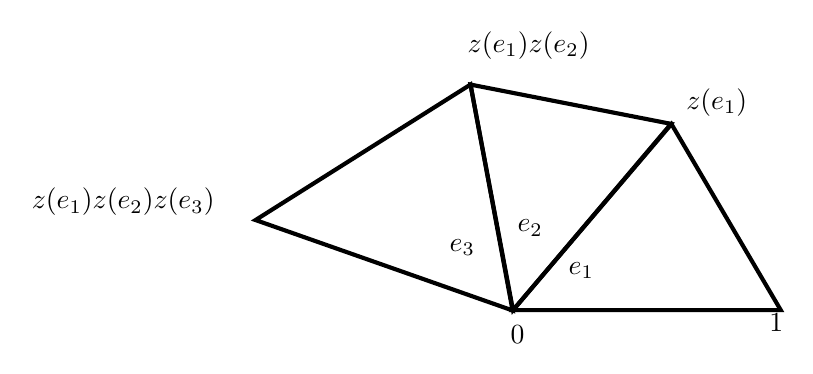
\begin{tikzpicture}[x=0.75pt,y=0.75pt,yscale=-1,xscale=1]
%uncomment if require: \path (0,300); %set diagram left start at 0, and has height of 300

%Shape: Triangle [id:dp3094193515878545] 
\draw  [line width=1.5]  (306.18,69.64) -- (402.79,88.57) -- (326.67,178.33) -- cycle ;
%Shape: Triangle [id:dp975605725949933] 
\draw  [line width=1.5]  (403,88.67) -- (455.67,178.33) -- (326.67,178.33) -- cycle ;
%Shape: Triangle [id:dp6752076580728734] 
\draw  [line width=1.5]  (326.45,178.47) -- (202.62,134.91) -- (306.18,69.64) -- cycle ;

% Text Node
\draw (352,154.07) node [anchor=north west][inner sep=0.75pt]    {$e_{1}$};
% Text Node
\draw (327.33,133.4) node [anchor=north west][inner sep=0.75pt]    {$e_{2}$};
% Text Node
\draw (294.67,142.73) node [anchor=north west][inner sep=0.75pt]    {$e_{3}$};
% Text Node
\draw (324,184.4) node [anchor=north west][inner sep=0.75pt]    {$0$};
% Text Node
\draw (448.67,178.73) node [anchor=north west][inner sep=0.75pt]    {$1$};
% Text Node
\draw (408.67,70.07) node [anchor=north west][inner sep=0.75pt]    {$z( e_{1})$};
% Text Node
\draw (303.33,42.73) node [anchor=north west][inner sep=0.75pt]    {$z( e_{1}) z( e_{2})$};
% Text Node
\draw (93.33,118.07) node [anchor=north west][inner sep=0.75pt]    {$z( e_{1}) z( e_{2}) z( e_{3})$};


\end{tikzpicture}
    \caption{Vertices de triangulos pegados}
\end{figure}
Observe que cada vez multiplicamos el invariante y dependiendo del angulo entre las caras del tetraedro se ira sumando un angulo diferente que en particular queremos que coincida con dar una vuelta completa, esta intuición justifica el siguiente teorema
\begin{theorem}
    Sea $M$ una 3-variedad que admite una triangulación topológica ideal tal que cada tetraedro tiene una estructura hiperbólica. La estructura hiperbólica en los tetraedros induce una estructura hiperbólica en el pegado si y solo si para cada arista $e$ tenemos que 
    $$\prod z(e_i)=1\quad\text{y}\quad\sum\arg z(e_i)=2\pi.$$
\end{theorem}
En primera instancia podríamos pensar que tenemos muchas variables, pero como todos los invariantes de aristas dependen de uno solo por el lema 4.1, cada tetraedro aporta a lo mas una variable. Con esta ecuación dotemos a nuestro ejemplo principal.
\begin{eg}
    Recordemos la descompocision en dos tetraedros ideales que ya teníamos del nudo de $8$
    \begin{figure}[H]
    \centering
    
%!TEX root = ./main.tex



\tikzset{every picture/.style={line width=0.75pt}} %set default line width to 0.75pt        

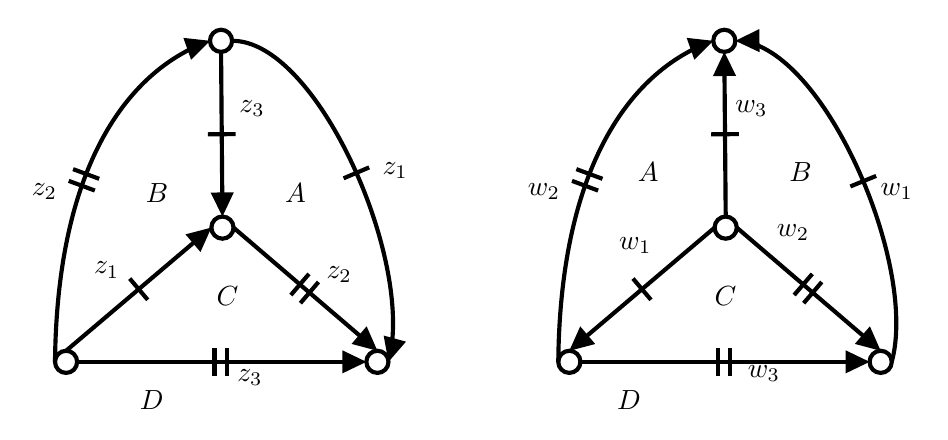
\begin{tikzpicture}[x=0.75pt,y=0.75pt,yscale=-1,xscale=1]
%uncomment if require: \path (0,877); %set diagram left start at 0, and has height of 877

%Shape: Circle [id:dp84958386512667] 
\draw  [line width=1.5]  (189.33,55.33) .. controls (189.33,52.39) and (191.72,50) .. (194.67,50) .. controls (197.61,50) and (200,52.39) .. (200,55.33) .. controls (200,58.28) and (197.61,60.67) .. (194.67,60.67) .. controls (191.72,60.67) and (189.33,58.28) .. (189.33,55.33) -- cycle ;
%Shape: Circle [id:dp7070798701116545] 
\draw  [line width=1.5]  (190,145.33) .. controls (190,142.39) and (192.39,140) .. (195.33,140) .. controls (198.28,140) and (200.67,142.39) .. (200.67,145.33) .. controls (200.67,148.28) and (198.28,150.67) .. (195.33,150.67) .. controls (192.39,150.67) and (190,148.28) .. (190,145.33) -- cycle ;
%Shape: Circle [id:dp5401287447911013] 
\draw  [line width=1.5]  (114.67,210) .. controls (114.67,207.05) and (117.05,204.67) .. (120,204.67) .. controls (122.95,204.67) and (125.33,207.05) .. (125.33,210) .. controls (125.33,212.95) and (122.95,215.33) .. (120,215.33) .. controls (117.05,215.33) and (114.67,212.95) .. (114.67,210) -- cycle ;
%Shape: Circle [id:dp024366460256337152] 
\draw  [line width=1.5]  (264.67,210) .. controls (264.67,207.05) and (267.05,204.67) .. (270,204.67) .. controls (272.95,204.67) and (275.33,207.05) .. (275.33,210) .. controls (275.33,212.95) and (272.95,215.33) .. (270,215.33) .. controls (267.05,215.33) and (264.67,212.95) .. (264.67,210) -- cycle ;
%Straight Lines [id:da5819091680445531] 
\draw [line width=1.5]    (194.67,60.67) -- (195.3,136) ;
\draw [shift={(195.33,140)}, rotate = 269.52] [fill={rgb, 255:red, 0; green, 0; blue, 0 }  ][line width=0.08]  [draw opacity=0] (11.61,-5.58) -- (0,0) -- (11.61,5.58) -- cycle    ;
\draw [shift={(195,100.33)}, rotate = 269.52] [color={rgb, 255:red, 0; green, 0; blue, 0 }  ][line width=1.5]    (0,6.71) -- (0,-6.71)   ;
%Straight Lines [id:da6153154443999455] 
\draw [line width=1.5]    (125.33,210) -- (260.67,210) ;
\draw [shift={(264.67,210)}, rotate = 180] [fill={rgb, 255:red, 0; green, 0; blue, 0 }  ][line width=0.08]  [draw opacity=0] (11.61,-5.58) -- (0,0) -- (11.61,5.58) -- cycle    ;
\draw [shift={(191.5,210)}, rotate = 180] [color={rgb, 255:red, 0; green, 0; blue, 0 }  ][line width=1.5]    (0,6.71) -- (0,-6.71)(-6.03,6.71) -- (-6.03,-6.71)   ;
%Straight Lines [id:da5399323102122296] 
\draw [line width=1.5]    (120,204.67) -- (186.95,147.92) ;
\draw [shift={(190,145.33)}, rotate = 139.71] [fill={rgb, 255:red, 0; green, 0; blue, 0 }  ][line width=0.08]  [draw opacity=0] (11.61,-5.58) -- (0,0) -- (11.61,5.58) -- cycle    ;
\draw [shift={(155,175)}, rotate = 139.71] [color={rgb, 255:red, 0; green, 0; blue, 0 }  ][line width=1.5]    (0,6.71) -- (0,-6.71)   ;
%Straight Lines [id:da7687719054145034] 
\draw [line width=1.5]    (200.67,145.33) -- (266.96,202.07) ;
\draw [shift={(270,204.67)}, rotate = 220.56] [fill={rgb, 255:red, 0; green, 0; blue, 0 }  ][line width=0.08]  [draw opacity=0] (11.61,-5.58) -- (0,0) -- (11.61,5.58) -- cycle    ;
\draw [shift={(232.67,172.72)}, rotate = 220.56] [color={rgb, 255:red, 0; green, 0; blue, 0 }  ][line width=1.5]    (0,6.71) -- (0,-6.71)(-6.03,6.71) -- (-6.03,-6.71)   ;
%Curve Lines [id:da44100647811810356] 
\draw [line width=1.5]    (114.67,210) .. controls (115.64,114.62) and (150.17,70.98) .. (186.01,56.59) ;
\draw [shift={(189.33,55.33)}, rotate = 160.64] [fill={rgb, 255:red, 0; green, 0; blue, 0 }  ][line width=0.08]  [draw opacity=0] (11.61,-5.58) -- (0,0) -- (11.61,5.58) -- cycle    ;
\draw [shift={(127.57,125.14)}, rotate = 110.35] [color={rgb, 255:red, 0; green, 0; blue, 0 }  ][line width=1.5]    (0,6.71) -- (0,-6.71)(-6.03,6.71) -- (-6.03,-6.71)   ;
%Curve Lines [id:da6379686625487593] 
\draw [line width=1.5]    (200,55.33) .. controls (239.98,55.01) and (285.97,157.03) .. (276.2,206.32) ;
\draw [shift={(275.33,210)}, rotate = 285.26] [fill={rgb, 255:red, 0; green, 0; blue, 0 }  ][line width=0.08]  [draw opacity=0] (11.61,-5.58) -- (0,0) -- (11.61,5.58) -- cycle    ;
\draw [shift={(259.87,118.95)}, rotate = 246.87] [color={rgb, 255:red, 0; green, 0; blue, 0 }  ][line width=1.5]    (0,6.71) -- (0,-6.71)   ;
%Shape: Circle [id:dp034440490903057674] 
\draw  [line width=1.5]  (431.81,55.33) .. controls (431.81,52.39) and (434.2,50) .. (437.14,50) .. controls (440.09,50) and (442.47,52.39) .. (442.47,55.33) .. controls (442.47,58.28) and (440.09,60.67) .. (437.14,60.67) .. controls (434.2,60.67) and (431.81,58.28) .. (431.81,55.33) -- cycle ;
%Shape: Circle [id:dp4739299080174333] 
\draw  [line width=1.5]  (432.47,145.33) .. controls (432.47,142.39) and (434.86,140) .. (437.81,140) .. controls (440.75,140) and (443.14,142.39) .. (443.14,145.33) .. controls (443.14,148.28) and (440.75,150.67) .. (437.81,150.67) .. controls (434.86,150.67) and (432.47,148.28) .. (432.47,145.33) -- cycle ;
%Shape: Circle [id:dp2986589831675226] 
\draw  [line width=1.5]  (357.14,210) .. controls (357.14,207.05) and (359.53,204.67) .. (362.47,204.67) .. controls (365.42,204.67) and (367.81,207.05) .. (367.81,210) .. controls (367.81,212.95) and (365.42,215.33) .. (362.47,215.33) .. controls (359.53,215.33) and (357.14,212.95) .. (357.14,210) -- cycle ;
%Shape: Circle [id:dp6438231834616311] 
\draw  [line width=1.5]  (507.14,210) .. controls (507.14,207.05) and (509.53,204.67) .. (512.47,204.67) .. controls (515.42,204.67) and (517.81,207.05) .. (517.81,210) .. controls (517.81,212.95) and (515.42,215.33) .. (512.47,215.33) .. controls (509.53,215.33) and (507.14,212.95) .. (507.14,210) -- cycle ;
%Straight Lines [id:da019687389237552866] 
\draw [line width=1.5]    (437.17,64.67) -- (437.81,140) ;
\draw [shift={(437.47,100.33)}, rotate = 269.52] [color={rgb, 255:red, 0; green, 0; blue, 0 }  ][line width=1.5]    (0,6.71) -- (0,-6.71)   ;
\draw [shift={(437.14,60.67)}, rotate = 89.52] [fill={rgb, 255:red, 0; green, 0; blue, 0 }  ][line width=0.08]  [draw opacity=0] (11.61,-5.58) -- (0,0) -- (11.61,5.58) -- cycle    ;
%Straight Lines [id:da5743118307270256] 
\draw [line width=1.5]    (367.81,210) -- (503.14,210) ;
\draw [shift={(507.14,210)}, rotate = 180] [fill={rgb, 255:red, 0; green, 0; blue, 0 }  ][line width=0.08]  [draw opacity=0] (11.61,-5.58) -- (0,0) -- (11.61,5.58) -- cycle    ;
\draw [shift={(433.97,210)}, rotate = 180] [color={rgb, 255:red, 0; green, 0; blue, 0 }  ][line width=1.5]    (0,6.71) -- (0,-6.71)(-6.03,6.71) -- (-6.03,-6.71)   ;
%Straight Lines [id:da15352339522122915] 
\draw [line width=1.5]    (365.53,202.08) -- (432.47,145.33) ;
\draw [shift={(397.47,175)}, rotate = 139.71] [color={rgb, 255:red, 0; green, 0; blue, 0 }  ][line width=1.5]    (0,6.71) -- (0,-6.71)   ;
\draw [shift={(362.47,204.67)}, rotate = 319.71] [fill={rgb, 255:red, 0; green, 0; blue, 0 }  ][line width=0.08]  [draw opacity=0] (11.61,-5.58) -- (0,0) -- (11.61,5.58) -- cycle    ;
%Straight Lines [id:da15958460866160962] 
\draw [line width=1.5]    (443.14,145.33) -- (509.43,202.07) ;
\draw [shift={(512.47,204.67)}, rotate = 220.56] [fill={rgb, 255:red, 0; green, 0; blue, 0 }  ][line width=0.08]  [draw opacity=0] (11.61,-5.58) -- (0,0) -- (11.61,5.58) -- cycle    ;
\draw [shift={(475.15,172.72)}, rotate = 220.56] [color={rgb, 255:red, 0; green, 0; blue, 0 }  ][line width=1.5]    (0,6.71) -- (0,-6.71)(-6.03,6.71) -- (-6.03,-6.71)   ;
%Curve Lines [id:da2355671835877725] 
\draw [line width=1.5]    (357.14,210) .. controls (358.11,114.62) and (392.64,70.98) .. (428.48,56.59) ;
\draw [shift={(431.81,55.33)}, rotate = 160.64] [fill={rgb, 255:red, 0; green, 0; blue, 0 }  ][line width=0.08]  [draw opacity=0] (11.61,-5.58) -- (0,0) -- (11.61,5.58) -- cycle    ;
\draw [shift={(370.05,125.14)}, rotate = 110.35] [color={rgb, 255:red, 0; green, 0; blue, 0 }  ][line width=1.5]    (0,6.71) -- (0,-6.71)(-6.03,6.71) -- (-6.03,-6.71)   ;
%Curve Lines [id:da10269880002458354] 
\draw [line width=1.5]    (446.8,55.69) .. controls (486.71,62.44) and (530.35,164) .. (517.81,210) ;
\draw [shift={(504.08,122.96)}, rotate = 247.81] [color={rgb, 255:red, 0; green, 0; blue, 0 }  ][line width=1.5]    (0,6.71) -- (0,-6.71)   ;
\draw [shift={(442.47,55.33)}, rotate = 359.53] [fill={rgb, 255:red, 0; green, 0; blue, 0 }  ][line width=0.08]  [draw opacity=0] (11.61,-5.58) -- (0,0) -- (11.61,5.58) -- cycle    ;

% Text Node
\draw (394,112.4) node [anchor=north west][inner sep=0.75pt]    {$A$};
% Text Node
\draw (467,112.4) node [anchor=north west][inner sep=0.75pt]    {$B$};
% Text Node
\draw (431,172.4) node [anchor=north west][inner sep=0.75pt]    {$C$};
% Text Node
\draw (384,222.4) node [anchor=north west][inner sep=0.75pt]    {$D$};
% Text Node
\draw (224,122.4) node [anchor=north west][inner sep=0.75pt]    {$A$};
% Text Node
\draw (157,122.4) node [anchor=north west][inner sep=0.75pt]    {$B$};
% Text Node
\draw (191,172.4) node [anchor=north west][inner sep=0.75pt]    {$C$};
% Text Node
\draw (154,222.4) node [anchor=north west][inner sep=0.75pt]    {$D$};
% Text Node
\draw (132,160.4) node [anchor=north west][inner sep=0.75pt]    {$z_{1}$};
% Text Node
\draw (271,112.4) node [anchor=north west][inner sep=0.75pt]    {$z_{1}$};
% Text Node
\draw (244,162.4) node [anchor=north west][inner sep=0.75pt]    {$z_{2}$};
% Text Node
\draw (102,122.4) node [anchor=north west][inner sep=0.75pt]    {$z_{2}$};
% Text Node
\draw (201,212.4) node [anchor=north west][inner sep=0.75pt]    {$z_{3}$};
% Text Node
\draw (202,82.4) node [anchor=north west][inner sep=0.75pt]    {$z_{3}$};
% Text Node
\draw (385,148.4) node [anchor=north west][inner sep=0.75pt]    {$w_{1}$};
% Text Node
\draw (511,122.4) node [anchor=north west][inner sep=0.75pt]    {$w_{1}$};
% Text Node
\draw (461,142.4) node [anchor=north west][inner sep=0.75pt]    {$w_{2}$};
% Text Node
\draw (341,122.4) node [anchor=north west][inner sep=0.75pt]    {$w_{2}$};
% Text Node
\draw (441,82.4) node [anchor=north west][inner sep=0.75pt]    {$w_{3}$};
% Text Node
\draw (447,210.4) node [anchor=north west][inner sep=0.75pt]    {$w_{3}$};


\end{tikzpicture}
        \caption{tetraedros ideales del nudo de 8 con invariantes de aristas}
    \end{figure}
    Observe que por ser mas consistentes cambiamos la vista del poliedro de arriba a la parte exterior, lo que ocasiona una reflexión en el diagrama obtenido antes, ademas observe que a cada arista la hemos dotado de un numero complejo $z_i$ y $w_i$, justamente este es el invariante de arista asociado a enviar esa arista a la arista que va de $0$ a $\infty$, note que por el primer ítem del lema 4.1 solo se necesitan tres indices en primera instancia. Así para cada arista tenemos respectivamente
    $$z_1^2z_3w_1^2w_3=1\quad\text{y}\quad z_2^2z_3w_2^2w_3=1.$$
    Observe que podemos simplificar aun mas usando los otros dos ítems, si $z_1=z$ y $w_1=w$, tenemos que las ecuaciones se convierten en
    $$z^2\frac{z-1}{z}w^2\frac{w-1}{w}=1\quad\text{y}\quad \frac{1}{(1-z)^2}\frac{z-1}{z}\frac{1}{(1-w)^2}\frac{w-1}{w}=1,$$
    Observe que en ambos casos esto se reduce a la única ecuación
    $$z(z-1)w(w-1)=1,$$
    por lo que si solucionamos la ecuación cuadrática en términos de $z$ las soluciones son
    $$z=\frac{1\pm\sqrt{1+\dfrac{4}{w(w-1)}}}{2},$$
    Esto nos determina las soluciones condicionadas netamente a $w$, primero recordemos que $w$ tiene parte imaginaria positiva por hipótesis, queremos de manera similar que $z$ tenga parte imaginaria positiva, esto se consigue siempre que $1+\dfrac{4}{w(w-1)}$ no sea un numero real positivo. Primero observe que es un numero real positivo si $\Im(w(w-1))= 0$, de aquí uno concluye que $\Re(w)=\dfrac{1}{2}$, y segundo necesitaríamos que $1+\dfrac{4}{w(w-1)}>0$, luego de algunas simplificaciones usando la condición anterior se llega a la cuadrática $4y^2-15>0$, donde $y=\Im(w)$, de ahí se concluye que $\Im(w)>\dfrac{\sqrt{15}}{2}$, por lo que nuestro conjunto de soluciones para $w$ que nos dan que $z$ tiene parte imaginaria positiva y dotan del pegado de una estructura hiperbólica es
    $$\bb{H}^2\setminus\left\{w\in\bb{C}:\Re(w)=\frac{1}{2}\quad\text{y}\quad \Im(w)>\frac{\sqrt{15}}{2}\right\}$$ 
\end{eg}

\subsection{Ecuaciones de Completez}
Antes solo observábamos el complemento del nudo, mas ahora la idea sera observar el exterior del nudo, ya que esto genera una frontera toroidal a la tres variedad y ademas la volverá compacta,, y es importante considerar estas cúspides para entender si hay una estructura hiperbólica completa.
\begin{definition}
    Sea $M$ una 3-variedad con frontera toroidal, definimos una cúspide de $M$, como una vecindad de la frontera que es homeomorfa a $T^2\times [0,\infty]$
\end{definition}

En un principio no resulta tan claro el como encontrar estas cúspides, mas en el caso de nuestra descompocision se pueden llegar a entender de una mejor manera

\begin{definition}
    Sea $M$ una 3-variedad que admite una triangulación topológica ideal, si truncamos los vértices de cada tetraedro ideal se obtiene una colección de triángulos, donde cada uno  se encuentra en la frontera de una cúspide, las aristas de cada triangulo adquieren un pegado natural dado por las caras del tetraedro. Esto nos da una triangulación de cada frontera toroidal. Que llamamos una triangulación de cúspide
\end{definition}

\begin{eg}
    Si truncamos los vértices de nuestra triangulación del complemento del nudo de $8$ obtenemos los siguientes triángulos ya pegados que justamente nos dan la identificación del toro
    \begin{figure}[H]
    \centering
    
%!TEX root = ./main.tex



\tikzset{every picture/.style={line width=0.75pt}} %set default line width to 0.75pt        

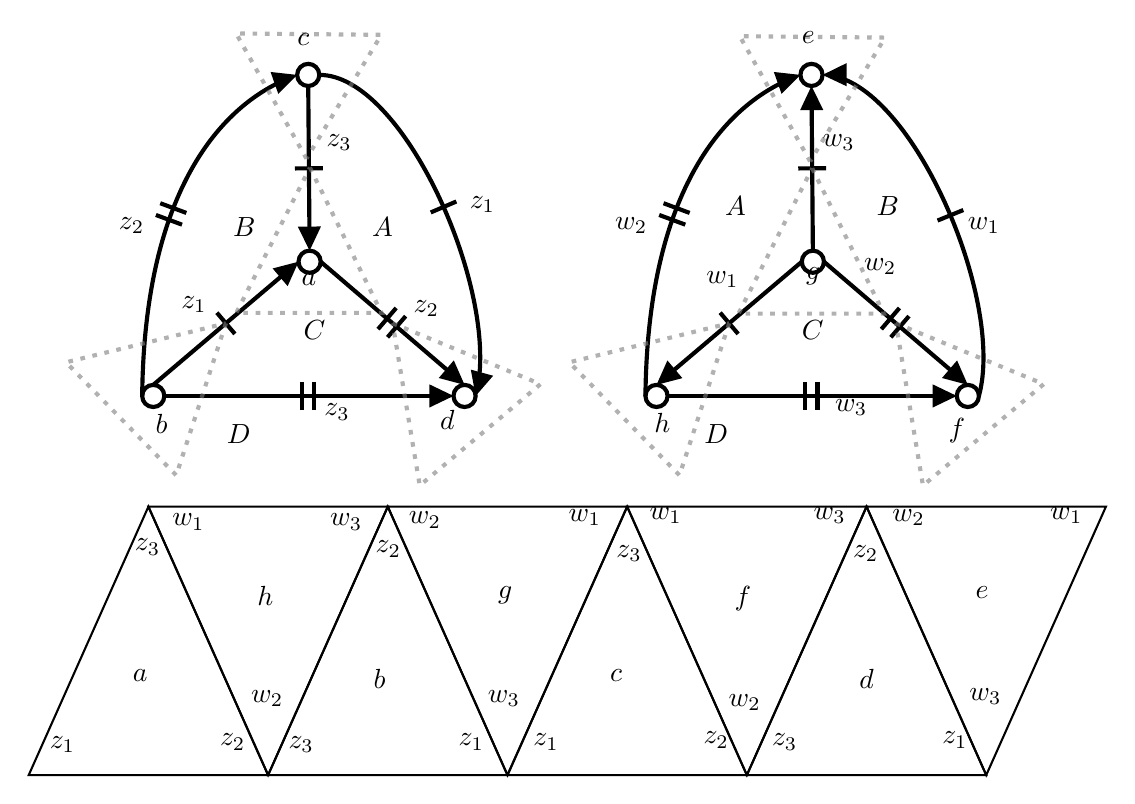
\begin{tikzpicture}[x=0.75pt,y=0.75pt,yscale=-1,xscale=1]
%uncomment if require: \path (0,877); %set diagram left start at 0, and has height of 877

%Shape: Circle [id:dp84958386512667] 
\draw  [line width=1.5]  (189.33,55.33) .. controls (189.33,52.39) and (191.72,50) .. (194.67,50) .. controls (197.61,50) and (200,52.39) .. (200,55.33) .. controls (200,58.28) and (197.61,60.67) .. (194.67,60.67) .. controls (191.72,60.67) and (189.33,58.28) .. (189.33,55.33) -- cycle ;
%Shape: Circle [id:dp7070798701116545] 
\draw  [line width=1.5]  (190,145.33) .. controls (190,142.39) and (192.39,140) .. (195.33,140) .. controls (198.28,140) and (200.67,142.39) .. (200.67,145.33) .. controls (200.67,148.28) and (198.28,150.67) .. (195.33,150.67) .. controls (192.39,150.67) and (190,148.28) .. (190,145.33) -- cycle ;
%Shape: Circle [id:dp5401287447911013] 
\draw  [line width=1.5]  (114.67,210) .. controls (114.67,207.05) and (117.05,204.67) .. (120,204.67) .. controls (122.95,204.67) and (125.33,207.05) .. (125.33,210) .. controls (125.33,212.95) and (122.95,215.33) .. (120,215.33) .. controls (117.05,215.33) and (114.67,212.95) .. (114.67,210) -- cycle ;
%Shape: Circle [id:dp024366460256337152] 
\draw  [line width=1.5]  (264.67,210) .. controls (264.67,207.05) and (267.05,204.67) .. (270,204.67) .. controls (272.95,204.67) and (275.33,207.05) .. (275.33,210) .. controls (275.33,212.95) and (272.95,215.33) .. (270,215.33) .. controls (267.05,215.33) and (264.67,212.95) .. (264.67,210) -- cycle ;
%Straight Lines [id:da5819091680445531] 
\draw [line width=1.5]    (194.67,60.67) -- (195.3,136) ;
\draw [shift={(195.33,140)}, rotate = 269.52] [fill={rgb, 255:red, 0; green, 0; blue, 0 }  ][line width=0.08]  [draw opacity=0] (11.61,-5.58) -- (0,0) -- (11.61,5.58) -- cycle    ;
\draw [shift={(195,100.33)}, rotate = 269.52] [color={rgb, 255:red, 0; green, 0; blue, 0 }  ][line width=1.5]    (0,6.71) -- (0,-6.71)   ;
%Straight Lines [id:da6153154443999455] 
\draw [line width=1.5]    (125.33,210) -- (260.67,210) ;
\draw [shift={(264.67,210)}, rotate = 180] [fill={rgb, 255:red, 0; green, 0; blue, 0 }  ][line width=0.08]  [draw opacity=0] (11.61,-5.58) -- (0,0) -- (11.61,5.58) -- cycle    ;
\draw [shift={(191.5,210)}, rotate = 180] [color={rgb, 255:red, 0; green, 0; blue, 0 }  ][line width=1.5]    (0,6.71) -- (0,-6.71)(-6.03,6.71) -- (-6.03,-6.71)   ;
%Straight Lines [id:da5399323102122296] 
\draw [line width=1.5]    (120,204.67) -- (186.95,147.92) ;
\draw [shift={(190,145.33)}, rotate = 139.71] [fill={rgb, 255:red, 0; green, 0; blue, 0 }  ][line width=0.08]  [draw opacity=0] (11.61,-5.58) -- (0,0) -- (11.61,5.58) -- cycle    ;
\draw [shift={(155,175)}, rotate = 139.71] [color={rgb, 255:red, 0; green, 0; blue, 0 }  ][line width=1.5]    (0,6.71) -- (0,-6.71)   ;
%Straight Lines [id:da7687719054145034] 
\draw [line width=1.5]    (200.67,145.33) -- (266.96,202.07) ;
\draw [shift={(270,204.67)}, rotate = 220.56] [fill={rgb, 255:red, 0; green, 0; blue, 0 }  ][line width=0.08]  [draw opacity=0] (11.61,-5.58) -- (0,0) -- (11.61,5.58) -- cycle    ;
\draw [shift={(232.67,172.72)}, rotate = 220.56] [color={rgb, 255:red, 0; green, 0; blue, 0 }  ][line width=1.5]    (0,6.71) -- (0,-6.71)(-6.03,6.71) -- (-6.03,-6.71)   ;
%Curve Lines [id:da44100647811810356] 
\draw [line width=1.5]    (114.67,210) .. controls (115.64,114.62) and (150.17,70.98) .. (186.01,56.59) ;
\draw [shift={(189.33,55.33)}, rotate = 160.64] [fill={rgb, 255:red, 0; green, 0; blue, 0 }  ][line width=0.08]  [draw opacity=0] (11.61,-5.58) -- (0,0) -- (11.61,5.58) -- cycle    ;
\draw [shift={(127.57,125.14)}, rotate = 110.35] [color={rgb, 255:red, 0; green, 0; blue, 0 }  ][line width=1.5]    (0,6.71) -- (0,-6.71)(-6.03,6.71) -- (-6.03,-6.71)   ;
%Curve Lines [id:da6379686625487593] 
\draw [line width=1.5]    (200,55.33) .. controls (239.98,55.01) and (285.97,157.03) .. (276.2,206.32) ;
\draw [shift={(275.33,210)}, rotate = 285.26] [fill={rgb, 255:red, 0; green, 0; blue, 0 }  ][line width=0.08]  [draw opacity=0] (11.61,-5.58) -- (0,0) -- (11.61,5.58) -- cycle    ;
\draw [shift={(259.87,118.95)}, rotate = 246.87] [color={rgb, 255:red, 0; green, 0; blue, 0 }  ][line width=1.5]    (0,6.71) -- (0,-6.71)   ;
%Shape: Circle [id:dp034440490903057674] 
\draw  [line width=1.5]  (431.81,55.33) .. controls (431.81,52.39) and (434.2,50) .. (437.14,50) .. controls (440.09,50) and (442.47,52.39) .. (442.47,55.33) .. controls (442.47,58.28) and (440.09,60.67) .. (437.14,60.67) .. controls (434.2,60.67) and (431.81,58.28) .. (431.81,55.33) -- cycle ;
%Shape: Circle [id:dp4739299080174333] 
\draw  [line width=1.5]  (432.47,145.33) .. controls (432.47,142.39) and (434.86,140) .. (437.81,140) .. controls (440.75,140) and (443.14,142.39) .. (443.14,145.33) .. controls (443.14,148.28) and (440.75,150.67) .. (437.81,150.67) .. controls (434.86,150.67) and (432.47,148.28) .. (432.47,145.33) -- cycle ;
%Shape: Circle [id:dp2986589831675226] 
\draw  [line width=1.5]  (357.14,210) .. controls (357.14,207.05) and (359.53,204.67) .. (362.47,204.67) .. controls (365.42,204.67) and (367.81,207.05) .. (367.81,210) .. controls (367.81,212.95) and (365.42,215.33) .. (362.47,215.33) .. controls (359.53,215.33) and (357.14,212.95) .. (357.14,210) -- cycle ;
%Shape: Circle [id:dp6438231834616311] 
\draw  [line width=1.5]  (507.14,210) .. controls (507.14,207.05) and (509.53,204.67) .. (512.47,204.67) .. controls (515.42,204.67) and (517.81,207.05) .. (517.81,210) .. controls (517.81,212.95) and (515.42,215.33) .. (512.47,215.33) .. controls (509.53,215.33) and (507.14,212.95) .. (507.14,210) -- cycle ;
%Straight Lines [id:da019687389237552866] 
\draw [line width=1.5]    (437.17,64.67) -- (437.81,140) ;
\draw [shift={(437.47,100.33)}, rotate = 269.52] [color={rgb, 255:red, 0; green, 0; blue, 0 }  ][line width=1.5]    (0,6.71) -- (0,-6.71)   ;
\draw [shift={(437.14,60.67)}, rotate = 89.52] [fill={rgb, 255:red, 0; green, 0; blue, 0 }  ][line width=0.08]  [draw opacity=0] (11.61,-5.58) -- (0,0) -- (11.61,5.58) -- cycle    ;
%Straight Lines [id:da5743118307270256] 
\draw [line width=1.5]    (367.81,210) -- (503.14,210) ;
\draw [shift={(507.14,210)}, rotate = 180] [fill={rgb, 255:red, 0; green, 0; blue, 0 }  ][line width=0.08]  [draw opacity=0] (11.61,-5.58) -- (0,0) -- (11.61,5.58) -- cycle    ;
\draw [shift={(433.97,210)}, rotate = 180] [color={rgb, 255:red, 0; green, 0; blue, 0 }  ][line width=1.5]    (0,6.71) -- (0,-6.71)(-6.03,6.71) -- (-6.03,-6.71)   ;
%Straight Lines [id:da15352339522122915] 
\draw [line width=1.5]    (365.53,202.08) -- (432.47,145.33) ;
\draw [shift={(397.47,175)}, rotate = 139.71] [color={rgb, 255:red, 0; green, 0; blue, 0 }  ][line width=1.5]    (0,6.71) -- (0,-6.71)   ;
\draw [shift={(362.47,204.67)}, rotate = 319.71] [fill={rgb, 255:red, 0; green, 0; blue, 0 }  ][line width=0.08]  [draw opacity=0] (11.61,-5.58) -- (0,0) -- (11.61,5.58) -- cycle    ;
%Straight Lines [id:da15958460866160962] 
\draw [line width=1.5]    (443.14,145.33) -- (509.43,202.07) ;
\draw [shift={(512.47,204.67)}, rotate = 220.56] [fill={rgb, 255:red, 0; green, 0; blue, 0 }  ][line width=0.08]  [draw opacity=0] (11.61,-5.58) -- (0,0) -- (11.61,5.58) -- cycle    ;
\draw [shift={(475.15,172.72)}, rotate = 220.56] [color={rgb, 255:red, 0; green, 0; blue, 0 }  ][line width=1.5]    (0,6.71) -- (0,-6.71)(-6.03,6.71) -- (-6.03,-6.71)   ;
%Curve Lines [id:da2355671835877725] 
\draw [line width=1.5]    (357.14,210) .. controls (358.11,114.62) and (392.64,70.98) .. (428.48,56.59) ;
\draw [shift={(431.81,55.33)}, rotate = 160.64] [fill={rgb, 255:red, 0; green, 0; blue, 0 }  ][line width=0.08]  [draw opacity=0] (11.61,-5.58) -- (0,0) -- (11.61,5.58) -- cycle    ;
\draw [shift={(370.05,125.14)}, rotate = 110.35] [color={rgb, 255:red, 0; green, 0; blue, 0 }  ][line width=1.5]    (0,6.71) -- (0,-6.71)(-6.03,6.71) -- (-6.03,-6.71)   ;
%Curve Lines [id:da10269880002458354] 
\draw [line width=1.5]    (446.8,55.69) .. controls (486.71,62.44) and (530.35,164) .. (517.81,210) ;
\draw [shift={(504.08,122.96)}, rotate = 247.81] [color={rgb, 255:red, 0; green, 0; blue, 0 }  ][line width=1.5]    (0,6.71) -- (0,-6.71)   ;
\draw [shift={(442.47,55.33)}, rotate = 359.53] [fill={rgb, 255:red, 0; green, 0; blue, 0 }  ][line width=0.08]  [draw opacity=0] (11.61,-5.58) -- (0,0) -- (11.61,5.58) -- cycle    ;
%Shape: Triangle [id:dp9575795612267674] 
\draw  [color={rgb, 255:red, 128; green, 128; blue, 128 }  ,draw opacity=0.61 ][dash pattern={on 1.69pt off 2.76pt}][line width=1.5]  (195.5,100) -- (230,170) -- (160,170) -- cycle ;
%Shape: Triangle [id:dp8304666288631158] 
\draw  [color={rgb, 255:red, 128; green, 128; blue, 128 }  ,draw opacity=0.61 ][dash pattern={on 1.69pt off 2.76pt}][line width=1.5]  (193.82,95.66) -- (159.91,35.34) -- (229.91,36.02) -- cycle ;
%Shape: Triangle [id:dp4999507729437477] 
\draw  [color={rgb, 255:red, 128; green, 128; blue, 128 }  ,draw opacity=0.61 ][dash pattern={on 1.69pt off 2.76pt}][line width=1.5]  (436.49,96.99) -- (402.58,36.67) -- (472.58,37.35) -- cycle ;
%Shape: Triangle [id:dp6286531931567367] 
\draw  [color={rgb, 255:red, 128; green, 128; blue, 128 }  ,draw opacity=0.61 ][dash pattern={on 1.69pt off 2.76pt}][line width=1.5]  (437.47,100.33) -- (471.97,170.33) -- (401.97,170.33) -- cycle ;
%Shape: Triangle [id:dp9402152936660696] 
\draw  [color={rgb, 255:red, 128; green, 128; blue, 128 }  ,draw opacity=0.61 ][dash pattern={on 1.69pt off 2.76pt}][line width=1.5]  (397.47,175) -- (373.53,248.23) -- (320.46,193.79) -- cycle ;
%Shape: Triangle [id:dp7181925212339698] 
\draw  [color={rgb, 255:red, 128; green, 128; blue, 128 }  ,draw opacity=0.61 ][dash pattern={on 1.69pt off 2.76pt}][line width=1.5]  (155,175) -- (131.06,248.23) -- (77.99,193.79) -- cycle ;
%Shape: Triangle [id:dp23139624969110628] 
\draw  [color={rgb, 255:red, 128; green, 128; blue, 128 }  ,draw opacity=0.61 ][dash pattern={on 1.69pt off 2.76pt}][line width=1.5]  (235.33,175) -- (306.59,204.29) -- (248.38,253.19) -- cycle ;
%Shape: Triangle [id:dp7463486020980554] 
\draw  [color={rgb, 255:red, 128; green, 128; blue, 128 }  ,draw opacity=0.61 ][dash pattern={on 1.69pt off 2.76pt}][line width=1.5]  (477.81,175) -- (549.07,204.29) -- (490.85,253.19) -- cycle ;
%Shape: Triangle [id:dp670762646815206] 
\draw   (117.67,263.33) -- (175.33,392.67) -- (60,392.67) -- cycle ;
%Shape: Triangle [id:dp6096644924278205] 
\draw   (233,263.33) -- (290.67,392.67) -- (175.33,392.67) -- cycle ;
%Shape: Triangle [id:dp6132969216533539] 
\draw   (348.33,263.33) -- (406,392.67) -- (290.67,392.67) -- cycle ;
%Shape: Triangle [id:dp1957398112131299] 
\draw   (463.67,263.33) -- (521.33,392.67) -- (406,392.67) -- cycle ;
%Shape: Triangle [id:dp6822990842952337] 
\draw   (175.33,392.67) -- (117.67,263.33) -- (233,263.33) -- cycle ;
%Shape: Triangle [id:dp6962930689163636] 
\draw   (290.67,392.67) -- (233,263.33) -- (348.33,263.33) -- cycle ;
%Shape: Triangle [id:dp1424783735549131] 
\draw   (406,392.67) -- (348.33,263.33) -- (463.67,263.33) -- cycle ;
%Shape: Triangle [id:dp3424699931659767] 
\draw   (521.33,392.67) -- (463.67,263.33) -- (579,263.33) -- cycle ;

% Text Node
\draw (394,112.4) node [anchor=north west][inner sep=0.75pt]    {$A$};
% Text Node
\draw (467,112.4) node [anchor=north west][inner sep=0.75pt]    {$B$};
% Text Node
\draw (431,172.4) node [anchor=north west][inner sep=0.75pt]    {$C$};
% Text Node
\draw (384,222.4) node [anchor=north west][inner sep=0.75pt]    {$D$};
% Text Node
\draw (224,122.4) node [anchor=north west][inner sep=0.75pt]    {$A$};
% Text Node
\draw (157,122.4) node [anchor=north west][inner sep=0.75pt]    {$B$};
% Text Node
\draw (191,172.4) node [anchor=north west][inner sep=0.75pt]    {$C$};
% Text Node
\draw (154,222.4) node [anchor=north west][inner sep=0.75pt]    {$D$};
% Text Node
\draw (132,160.4) node [anchor=north west][inner sep=0.75pt]    {$z_{1}$};
% Text Node
\draw (271,112.4) node [anchor=north west][inner sep=0.75pt]    {$z_{1}$};
% Text Node
\draw (244,162.4) node [anchor=north west][inner sep=0.75pt]    {$z_{2}$};
% Text Node
\draw (102,122.4) node [anchor=north west][inner sep=0.75pt]    {$z_{2}$};
% Text Node
\draw (201,212.4) node [anchor=north west][inner sep=0.75pt]    {$z_{3}$};
% Text Node
\draw (202,82.4) node [anchor=north west][inner sep=0.75pt]    {$z_{3}$};
% Text Node
\draw (385,148.4) node [anchor=north west][inner sep=0.75pt]    {$w_{1}$};
% Text Node
\draw (511,122.4) node [anchor=north west][inner sep=0.75pt]    {$w_{1}$};
% Text Node
\draw (461,142.4) node [anchor=north west][inner sep=0.75pt]    {$w_{2}$};
% Text Node
\draw (341,122.4) node [anchor=north west][inner sep=0.75pt]    {$w_{2}$};
% Text Node
\draw (441,82.4) node [anchor=north west][inner sep=0.75pt]    {$w_{3}$};
% Text Node
\draw (447,210.4) node [anchor=north west][inner sep=0.75pt]    {$w_{3}$};
% Text Node
\draw (190,149.4) node [anchor=north west][inner sep=0.75pt]    {$a$};
% Text Node
\draw (119.67,217.4) node [anchor=north west][inner sep=0.75pt]    {$b$};
% Text Node
\draw (256.67,215.4) node [anchor=north west][inner sep=0.75pt]    {$d$};
% Text Node
\draw (188,33.73) node [anchor=north west][inner sep=0.75pt]    {$c$};
% Text Node
\draw (431,33.07) node [anchor=north west][inner sep=0.75pt]    {$e$};
% Text Node
\draw (501.67,219.07) node [anchor=north west][inner sep=0.75pt]    {$f$};
% Text Node
\draw (433,146.73) node [anchor=north west][inner sep=0.75pt]    {$g$};
% Text Node
\draw (360,216.73) node [anchor=north west][inner sep=0.75pt]    {$h$};
% Text Node
\draw (108.67,340.4) node [anchor=north west][inner sep=0.75pt]    {$a$};
% Text Node
\draw (168.67,300.4) node [anchor=north west][inner sep=0.75pt]    {$h$};
% Text Node
\draw (224.67,340.4) node [anchor=north west][inner sep=0.75pt]    {$b$};
% Text Node
\draw (284.67,300.4) node [anchor=north west][inner sep=0.75pt]    {$g$};
% Text Node
\draw (338.67,340.4) node [anchor=north west][inner sep=0.75pt]    {$c$};
% Text Node
\draw (458.67,340.4) node [anchor=north west][inner sep=0.75pt]    {$d$};
% Text Node
\draw (398.67,300.4) node [anchor=north west][inner sep=0.75pt]    {$f$};
% Text Node
\draw (514.67,300.4) node [anchor=north west][inner sep=0.75pt]    {$e$};
% Text Node
\draw (68.67,372.4) node [anchor=north west][inner sep=0.75pt]    {$z_{1}$};
% Text Node
\draw (150.67,371.4) node [anchor=north west][inner sep=0.75pt]    {$z_{2}$};
% Text Node
\draw (183.67,372.4) node [anchor=north west][inner sep=0.75pt]    {$z_{3}$};
% Text Node
\draw (265.67,371.4) node [anchor=north west][inner sep=0.75pt]    {$z_{1}$};
% Text Node
\draw (301.67,371.4) node [anchor=north west][inner sep=0.75pt]    {$z_{1}$};
% Text Node
\draw (383.67,370.4) node [anchor=north west][inner sep=0.75pt]    {$z_{2}$};
% Text Node
\draw (416.67,371.4) node [anchor=north west][inner sep=0.75pt]    {$z_{3}$};
% Text Node
\draw (498.67,370.4) node [anchor=north west][inner sep=0.75pt]    {$z_{1}$};
% Text Node
\draw (127.67,265.4) node [anchor=north west][inner sep=0.75pt]    {$w_{1}$};
% Text Node
\draw (203.67,265.4) node [anchor=north west][inner sep=0.75pt]    {$w_{3}$};
% Text Node
\draw (241.67,264.4) node [anchor=north west][inner sep=0.75pt]    {$w_{2}$};
% Text Node
\draw (318.67,263.4) node [anchor=north west][inner sep=0.75pt]    {$w_{1}$};
% Text Node
\draw (357.67,262.4) node [anchor=north west][inner sep=0.75pt]    {$w_{1}$};
% Text Node
\draw (436.67,262.4) node [anchor=north west][inner sep=0.75pt]    {$w_{3}$};
% Text Node
\draw (474.67,263.4) node [anchor=north west][inner sep=0.75pt]    {$w_{2}$};
% Text Node
\draw (550.67,262.4) node [anchor=north west][inner sep=0.75pt]    {$w_{1}$};
% Text Node
\draw (165.67,350.4) node [anchor=north west][inner sep=0.75pt]    {$w_{2}$};
% Text Node
\draw (279.67,350.4) node [anchor=north west][inner sep=0.75pt]    {$w_{3}$};
% Text Node
\draw (395.67,352.4) node [anchor=north west][inner sep=0.75pt]    {$w_{2}$};
% Text Node
\draw (511.67,349.4) node [anchor=north west][inner sep=0.75pt]    {$w_{3}$};
% Text Node
\draw (109.67,277.4) node [anchor=north west][inner sep=0.75pt]    {$z_{3}$};
% Text Node
\draw (341.67,280.4) node [anchor=north west][inner sep=0.75pt]    {$z_{3}$};
% Text Node
\draw (225.67,278.4) node [anchor=north west][inner sep=0.75pt]    {$z_{2}$};
% Text Node
\draw (455.67,280.4) node [anchor=north west][inner sep=0.75pt]    {$z_{2}$};


\end{tikzpicture}
        \caption{Triangulación de la cuspide}
    
    \end{figure}
\end{eg}

Necesitamos de estas cúspides para el siguiente teorema que nos habla acerca de la completez de nuestra estructura inducida

\begin{theorem}
    Sea $M$ una 3-variedad con frontera toroidal y una estructura hiperbólica, esta estructura es completa en $M$ si y solo si la estructura inducida en cada frontera de una cúspide es una estructura euclidea sobre el toro.
\end{theorem}

Esto quiere decir que en el momento del pegado solo basta por preocuparnos por que la estructura hiperbólica del complemento de nuestro nudo, induzca una estructura euclidea en la triangulación de la cúspide, la pregunta es como podemos asegurar esto.

\begin{definition}
    Suponga que la 3-variedad $M$ posee una triangulación topológica ideal, y sea $T$ la frontera toroidal de una cuspide de $M$, sea $[\alpha]\in\pi_1(T)$, asociamos el numero $H(\alpha)$ de la siguiente manera. Dotando a $\alpha$ de una orientación, este por homotopia puede ser colocado de tal manera que en cada triangulo solo separe una esquina una vez, donde cada vértice esta dotado de un invariante de arista $z_i$, y como tiene orientación se puede determinar si esta a la izquierda o la derecha, esto lo determinaremos con una potencia $\epsilon_i=\pm 1$, positivo si esta a la izquierda y negativo en otro caso. Así 
    $$H(\alpha)=\prod_{i=1}^n z_i^{\epsilon_i},$$
\end{definition}
Tan extraño y misterioso como puede parecer este numero nos permite determinar cuando nuestra estructura hiperbólica es completa
\begin{theorem}
    Sea $T$ la frontera toroidal de una cúspide de $M$, donde $M$ admite una triangulación topológica ideal y los tetraedros ideales admiten una estructura hiperbólica que satisface las ecuaciones de pegado. Sean $\alpha$ y $\beta$ curvas que generan $\pi_1(T)$, si $H(\alpha)=H(\beta)=1$ entonces la triangulación es una triangulación ideal geométrica.
\end{theorem}

En estos últimos dos conceptos no se ahondo en sus justificaciones debido a que estas requieren herramientas de holonomia y funciones de de desarrollo, las cuales se salen un poco del propósito de este proyecto. Con esta herramienta que llamaremos ecuaciones de completez descubramos para que invariantes de arista el complemento del nudo de 8 posee una estructura hiperbólica completa

\begin{eg}
    Observe primero que dada la triangulación anterior basta con tomar las siguientes dos curvas que claramente generan el grupo fundamental
    \begin{figure}[H]
    \centering
    
%!TEX root = ./main.tex



\tikzset{every picture/.style={line width=0.75pt}} %set default line width to 0.75pt        

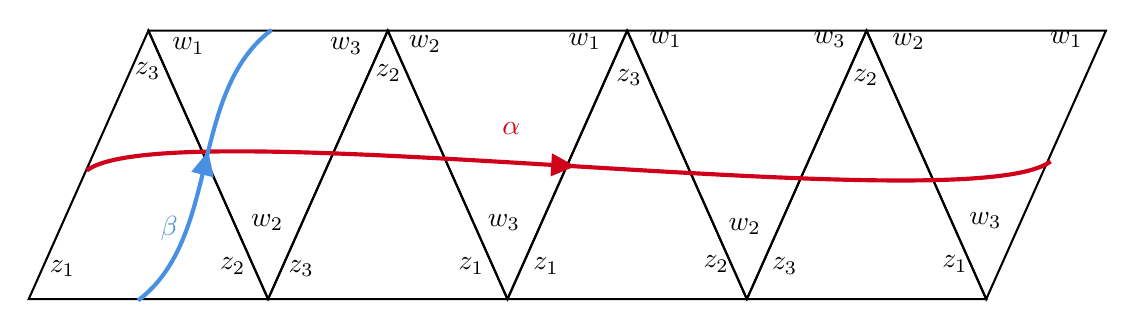
\begin{tikzpicture}[x=0.75pt,y=0.75pt,yscale=-1,xscale=1]
%uncomment if require: \path (0,877); %set diagram left start at 0, and has height of 877

%Shape: Triangle [id:dp670762646815206] 
\draw   (117.67,43.33) -- (175.33,172.67) -- (60,172.67) -- cycle ;
%Shape: Triangle [id:dp6096644924278205] 
\draw   (233,43.33) -- (290.67,172.67) -- (175.33,172.67) -- cycle ;
%Shape: Triangle [id:dp6132969216533539] 
\draw   (348.33,43.33) -- (406,172.67) -- (290.67,172.67) -- cycle ;
%Shape: Triangle [id:dp1957398112131299] 
\draw   (463.67,43.33) -- (521.33,172.67) -- (406,172.67) -- cycle ;
%Shape: Triangle [id:dp6822990842952337] 
\draw   (175.33,172.67) -- (117.67,43.33) -- (233,43.33) -- cycle ;
%Shape: Triangle [id:dp6962930689163636] 
\draw   (290.67,172.67) -- (233,43.33) -- (348.33,43.33) -- cycle ;
%Shape: Triangle [id:dp1424783735549131] 
\draw   (406,172.67) -- (348.33,43.33) -- (463.67,43.33) -- cycle ;
%Shape: Triangle [id:dp3424699931659767] 
\draw   (521.33,172.67) -- (463.67,43.33) -- (579,43.33) -- cycle ;
%Curve Lines [id:da21318320003967128] 
\draw [color={rgb, 255:red, 208; green, 2; blue, 27 }  ,draw opacity=1 ][line width=1.5]    (88,110.67) .. controls (128,80.67) and (512.33,136.33) .. (552.33,106.33) ;
\draw [shift={(323.35,108.69)}, rotate = 183.46] [fill={rgb, 255:red, 208; green, 2; blue, 27 }  ,fill opacity=1 ][line width=0.08]  [draw opacity=0] (11.61,-5.58) -- (0,0) -- (11.61,5.58) -- cycle    ;
%Curve Lines [id:da5420489243511813] 
\draw [color={rgb, 255:red, 74; green, 144; blue, 226 }  ,draw opacity=1 ][line width=1.5]    (112.67,173.33) .. controls (152.67,143.33) and (137,73) .. (177,43) ;
\draw [shift={(146.49,101.4)}, rotate = 103.75] [fill={rgb, 255:red, 74; green, 144; blue, 226 }  ,fill opacity=1 ][line width=0.08]  [draw opacity=0] (11.61,-5.58) -- (0,0) -- (11.61,5.58) -- cycle    ;

% Text Node
\draw (68.67,152.4) node [anchor=north west][inner sep=0.75pt]    {$z_{1}$};
% Text Node
\draw (150.67,151.4) node [anchor=north west][inner sep=0.75pt]    {$z_{2}$};
% Text Node
\draw (183.67,152.4) node [anchor=north west][inner sep=0.75pt]    {$z_{3}$};
% Text Node
\draw (265.67,151.4) node [anchor=north west][inner sep=0.75pt]    {$z_{1}$};
% Text Node
\draw (301.67,151.4) node [anchor=north west][inner sep=0.75pt]    {$z_{1}$};
% Text Node
\draw (383.67,150.4) node [anchor=north west][inner sep=0.75pt]    {$z_{2}$};
% Text Node
\draw (416.67,151.4) node [anchor=north west][inner sep=0.75pt]    {$z_{3}$};
% Text Node
\draw (498.67,150.4) node [anchor=north west][inner sep=0.75pt]    {$z_{1}$};
% Text Node
\draw (127.67,45.4) node [anchor=north west][inner sep=0.75pt]    {$w_{1}$};
% Text Node
\draw (203.67,45.4) node [anchor=north west][inner sep=0.75pt]    {$w_{3}$};
% Text Node
\draw (241.67,44.4) node [anchor=north west][inner sep=0.75pt]    {$w_{2}$};
% Text Node
\draw (318.67,43.4) node [anchor=north west][inner sep=0.75pt]    {$w_{1}$};
% Text Node
\draw (357.67,42.4) node [anchor=north west][inner sep=0.75pt]    {$w_{1}$};
% Text Node
\draw (436.67,42.4) node [anchor=north west][inner sep=0.75pt]    {$w_{3}$};
% Text Node
\draw (474.67,43.4) node [anchor=north west][inner sep=0.75pt]    {$w_{2}$};
% Text Node
\draw (550.67,42.4) node [anchor=north west][inner sep=0.75pt]    {$w_{1}$};
% Text Node
\draw (165.67,130.4) node [anchor=north west][inner sep=0.75pt]    {$w_{2}$};
% Text Node
\draw (279.67,130.4) node [anchor=north west][inner sep=0.75pt]    {$w_{3}$};
% Text Node
\draw (395.67,132.4) node [anchor=north west][inner sep=0.75pt]    {$w_{2}$};
% Text Node
\draw (511.67,129.4) node [anchor=north west][inner sep=0.75pt]    {$w_{3}$};
% Text Node
\draw (109.67,57.4) node [anchor=north west][inner sep=0.75pt]    {$z_{3}$};
% Text Node
\draw (341.67,60.4) node [anchor=north west][inner sep=0.75pt]    {$z_{3}$};
% Text Node
\draw (225.67,58.4) node [anchor=north west][inner sep=0.75pt]    {$z_{2}$};
% Text Node
\draw (455.67,60.4) node [anchor=north west][inner sep=0.75pt]    {$z_{2}$};
% Text Node
\draw (286.67,86.07) node [anchor=north west][inner sep=0.75pt]    {$\textcolor[rgb]{0.82,0.01,0.11}{\alpha }$};
% Text Node
\draw (122,131.4) node [anchor=north west][inner sep=0.75pt]    {$\textcolor[rgb]{0.29,0.56,0.89}{\beta }$};


\end{tikzpicture}
        \caption{Curvas $\alpha$ y $\beta$}
    \end{figure}
    Luego por la descripción dada antes $$H(\alpha)=z_3w_2^{-1}z_2w_3^{-1}z_3w_2^{-1}z_2w_3^{-1}=\left(\dfrac{z_2z_3}{w_2w_3}\right)^2$$, y $$H(\beta)=z_2^{-1}w_1=\dfrac{w_1}{z_2}$$
    Siguiendo el lema 4.1 si el invariante de arista $z_1=z$ y $w_1=w$  obtenemos que 
    $$H(\alpha)=\left(\frac{1}{1-z}\cdot\frac{z-1}{z}\cdot(1-w)\cdot\frac{w}{w-1}\right)^2=\frac{w^2}{z^2},$$
    y ademas $H(\beta)=w(1-z)$, por las ecuaciones de completez, como $H(\alpha)=1$, tenemos que $w^2=z^2$, luego $(w-z)(w+z)=0$, pero como $w$ y $z$ tienen parte imaginaria positiva el segundo factor no puede ser 0, luego $w=z$, sustituyendo esto en $H(\beta)=1$, obtenemos que $z^2-z+1=0$, luego la única posibilidad es que
    $$w=z=\frac{1}{2}+i\frac{\sqrt{3}}{2}$$
    el cual es justamente un punto de los puntos que si dotan de estructura hiperbólica, esto nos dice que todos los demás pegados no tienen estructura hiperbólica completa.
\end{eg}

\subsection{Ecuaciones de pegado para el nudo $6_1$}

Recordemos que antes ya habíamos hecho la descompocision del nudo $6_1$ en dos poliedros ideales los cuales si bien no son tetraedros, la forma en que están proyectados se asemeja mucho a unos, por lo que es natural preguntarse de que forma podemos convertir estos en tetraedros ideales, la idea sera tomar un vértices de uno de los poliedros en las caras que no son triángulos y luego conectar este con aquellos vértices con los que no tenga aristas, para subdividir la cara en triángulos, entonces dadas las proyecciones obtenidas previamente tenemos las siguientes subdivisiones
\begin{figure}[H]
\centering
%!TEX root = ./main.tex



\tikzset{every picture/.style={line width=0.75pt}} %set default line width to 0.75pt        

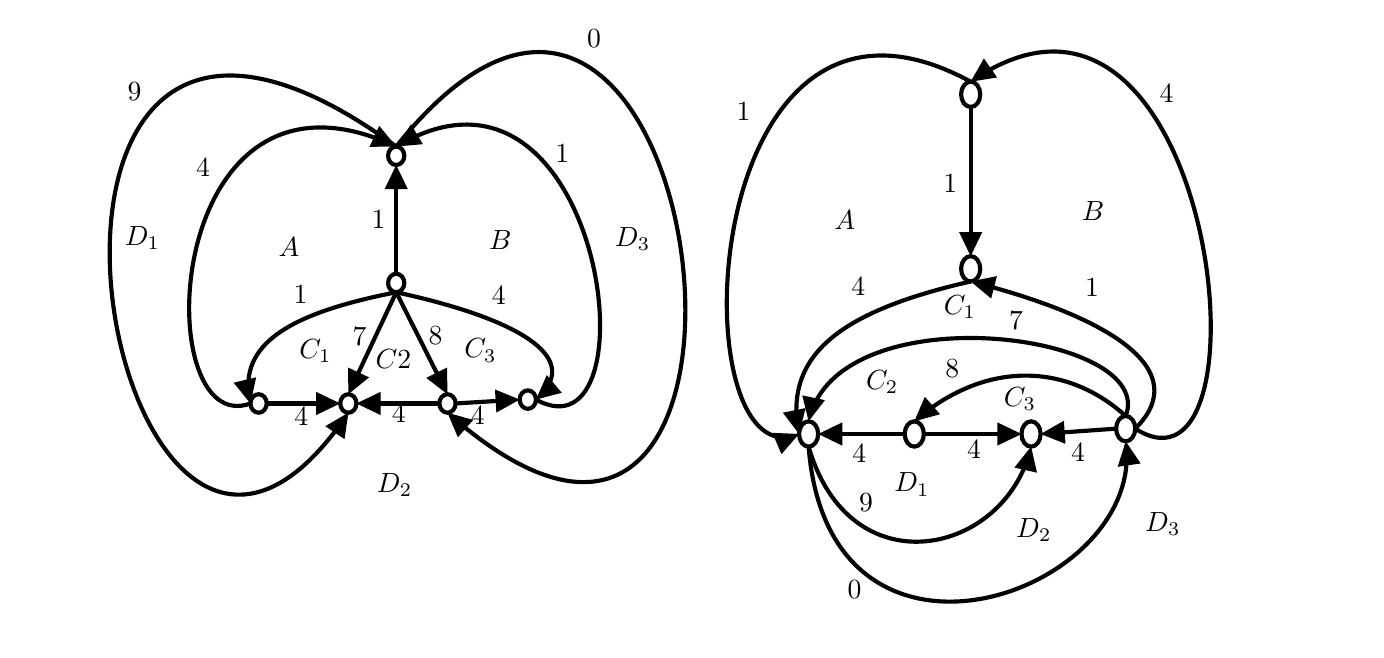
\begin{tikzpicture}[x=0.75pt,y=0.75pt,yscale=-1,xscale=1]
%uncomment if require: \path (0,331); %set diagram left start at 0, and has height of 331
\path[use as bounding box] (20,10) rectangle (660,300);
%Shape: Ellipse [id:dp012401419565516214] 
\draw  [color={rgb, 255:red, 0; green, 0; blue, 0 }  ,draw opacity=1 ][line width=1.5]  (193.64,71.71) .. controls (193.64,69.26) and (195.4,67.27) .. (197.56,67.27) .. controls (199.72,67.27) and (201.47,69.26) .. (201.47,71.71) .. controls (201.47,74.17) and (199.72,76.16) .. (197.56,76.16) .. controls (195.4,76.16) and (193.64,74.17) .. (193.64,71.71) -- cycle ;
%Shape: Ellipse [id:dp44563585877978507] 
\draw  [color={rgb, 255:red, 0; green, 0; blue, 0 }  ,draw opacity=1 ][line width=1.5]  (193.64,133.02) .. controls (193.64,130.56) and (195.4,128.57) .. (197.56,128.57) .. controls (199.72,128.57) and (201.47,130.56) .. (201.47,133.02) .. controls (201.47,135.47) and (199.72,137.47) .. (197.56,137.47) .. controls (195.4,137.47) and (193.64,135.47) .. (193.64,133.02) -- cycle ;
%Shape: Ellipse [id:dp12283994981009283] 
\draw  [color={rgb, 255:red, 0; green, 0; blue, 0 }  ,draw opacity=1 ][line width=1.5]  (127.35,191.05) .. controls (127.35,188.6) and (129.1,186.61) .. (131.26,186.61) .. controls (133.42,186.61) and (135.17,188.6) .. (135.17,191.05) .. controls (135.17,193.51) and (133.42,195.5) .. (131.26,195.5) .. controls (129.1,195.5) and (127.35,193.51) .. (127.35,191.05) -- cycle ;
%Shape: Ellipse [id:dp43640670243388857] 
\draw  [color={rgb, 255:red, 0; green, 0; blue, 0 }  ,draw opacity=1 ][line width=1.5]  (257.06,189.18) .. controls (257.06,186.72) and (258.81,184.73) .. (260.97,184.73) .. controls (263.13,184.73) and (264.88,186.72) .. (264.88,189.18) .. controls (264.88,191.63) and (263.13,193.63) .. (260.97,193.63) .. controls (258.81,193.63) and (257.06,191.63) .. (257.06,189.18) -- cycle ;
%Shape: Ellipse [id:dp8232398640866994] 
\draw  [color={rgb, 255:red, 0; green, 0; blue, 0 }  ,draw opacity=1 ][line width=1.5]  (170.59,191.05) .. controls (170.59,188.6) and (172.34,186.61) .. (174.5,186.61) .. controls (176.66,186.61) and (178.41,188.6) .. (178.41,191.05) .. controls (178.41,193.51) and (176.66,195.5) .. (174.5,195.5) .. controls (172.34,195.5) and (170.59,193.51) .. (170.59,191.05) -- cycle ;
%Shape: Ellipse [id:dp43325876938835506] 
\draw  [color={rgb, 255:red, 0; green, 0; blue, 0 }  ,draw opacity=1 ][line width=1.5]  (218.35,191.05) .. controls (218.35,188.6) and (220.1,186.61) .. (222.26,186.61) .. controls (224.42,186.61) and (226.18,188.6) .. (226.18,191.05) .. controls (226.18,193.51) and (224.42,195.5) .. (222.26,195.5) .. controls (220.1,195.5) and (218.35,193.51) .. (218.35,191.05) -- cycle ;
%Curve Lines [id:da9923025827403492] 
\draw [color={rgb, 255:red, 0; green, 0; blue, 0 }  ,draw opacity=1 ][line width=1.5]    (126.57,186.85) .. controls (123.15,160.86) and (149.05,147.02) .. (197.56,137.47) ;
\draw [shift={(127.35,191.05)}, rotate = 256.57] [fill={rgb, 255:red, 0; green, 0; blue, 0 }  ,fill opacity=1 ][line width=0.08]  [draw opacity=0] (11.61,-5.58) -- (0,0) -- (11.61,5.58) -- cycle    ;
%Curve Lines [id:da25092915579525166] 
\draw [color={rgb, 255:red, 0; green, 0; blue, 0 }  ,draw opacity=1 ][line width=1.5]    (267.85,186.35) .. controls (286.23,166.45) and (250.25,148.86) .. (197.56,137.47) ;
\draw [shift={(264.88,189.18)}, rotate = 319.56] [fill={rgb, 255:red, 0; green, 0; blue, 0 }  ,fill opacity=1 ][line width=0.08]  [draw opacity=0] (11.61,-5.58) -- (0,0) -- (11.61,5.58) -- cycle    ;
%Curve Lines [id:da6555373806548633] 
\draw [color={rgb, 255:red, 0; green, 0; blue, 0 }  ,draw opacity=1 ][line width=1.5]    (264.88,189.18) .. controls (322.57,220.69) and (298.52,11.84) .. (200.55,65.56) ;
\draw [shift={(197.56,67.27)}, rotate = 329.29] [fill={rgb, 255:red, 0; green, 0; blue, 0 }  ,fill opacity=1 ][line width=0.08]  [draw opacity=0] (11.61,-5.58) -- (0,0) -- (11.61,5.58) -- cycle    ;
%Curve Lines [id:da7978745153273987] 
\draw [color={rgb, 255:red, 0; green, 0; blue, 0 }  ,draw opacity=1 ][line width=1.5]    (127.35,191.05) .. controls (78.23,209.12) and (83.79,18.03) .. (194.18,65.75) ;
\draw [shift={(197.56,67.27)}, rotate = 205.05] [fill={rgb, 255:red, 0; green, 0; blue, 0 }  ,fill opacity=1 ][line width=0.08]  [draw opacity=0] (11.61,-5.58) -- (0,0) -- (11.61,5.58) -- cycle    ;
%Straight Lines [id:da8527204625447116] 
\draw [color={rgb, 255:red, 0; green, 0; blue, 0 }  ,draw opacity=1 ][line width=1.5]    (135.17,191.05) -- (166.59,191.05) ;
\draw [shift={(170.59,191.05)}, rotate = 180] [fill={rgb, 255:red, 0; green, 0; blue, 0 }  ,fill opacity=1 ][line width=0.08]  [draw opacity=0] (11.61,-5.58) -- (0,0) -- (11.61,5.58) -- cycle    ;
%Straight Lines [id:da24688497873734994] 
\draw [color={rgb, 255:red, 0; green, 0; blue, 0 }  ,draw opacity=1 ][line width=1.5]    (182.41,191.05) -- (218.35,191.05) ;
\draw [shift={(178.41,191.05)}, rotate = 0] [fill={rgb, 255:red, 0; green, 0; blue, 0 }  ,fill opacity=1 ][line width=0.08]  [draw opacity=0] (11.61,-5.58) -- (0,0) -- (11.61,5.58) -- cycle    ;
%Straight Lines [id:da7578777207736729] 
\draw [color={rgb, 255:red, 0; green, 0; blue, 0 }  ,draw opacity=1 ][line width=1.5]    (226.18,191.05) -- (253.07,189.42) ;
\draw [shift={(257.06,189.18)}, rotate = 176.53] [fill={rgb, 255:red, 0; green, 0; blue, 0 }  ,fill opacity=1 ][line width=0.08]  [draw opacity=0] (11.61,-5.58) -- (0,0) -- (11.61,5.58) -- cycle    ;
%Straight Lines [id:da9029001126541812] 
\draw [color={rgb, 255:red, 0; green, 0; blue, 0 }  ,draw opacity=1 ][line width=1.5]    (197.56,128.57) -- (197.56,80.16) ;
\draw [shift={(197.56,76.16)}, rotate = 90] [fill={rgb, 255:red, 0; green, 0; blue, 0 }  ,fill opacity=1 ][line width=0.08]  [draw opacity=0] (11.61,-5.58) -- (0,0) -- (11.61,5.58) -- cycle    ;
%Shape: Ellipse [id:dp0659583824499258] 
\draw  [color={rgb, 255:red, 0; green, 0; blue, 0 }  ,draw opacity=1 ][line width=1.5]  (469.72,42.1) .. controls (469.72,38.74) and (471.79,36.01) .. (474.33,36.01) .. controls (476.88,36.01) and (478.94,38.74) .. (478.94,42.1) .. controls (478.94,45.47) and (476.88,48.2) .. (474.33,48.2) .. controls (471.79,48.2) and (469.72,45.47) .. (469.72,42.1) -- cycle ;
%Shape: Ellipse [id:dp3071305848970848] 
\draw  [color={rgb, 255:red, 0; green, 0; blue, 0 }  ,draw opacity=1 ][line width=1.5]  (469.72,126.18) .. controls (469.72,122.81) and (471.79,120.08) .. (474.33,120.08) .. controls (476.88,120.08) and (478.94,122.81) .. (478.94,126.18) .. controls (478.94,129.54) and (476.88,132.27) .. (474.33,132.27) .. controls (471.79,132.27) and (469.72,129.54) .. (469.72,126.18) -- cycle ;
%Shape: Ellipse [id:dp762429770691099] 
\draw  [color={rgb, 255:red, 0; green, 0; blue, 0 }  ,draw opacity=1 ][line width=1.5]  (391.65,205.76) .. controls (391.65,202.39) and (393.71,199.66) .. (396.25,199.66) .. controls (398.8,199.66) and (400.86,202.39) .. (400.86,205.76) .. controls (400.86,209.12) and (398.8,211.85) .. (396.25,211.85) .. controls (393.71,211.85) and (391.65,209.12) .. (391.65,205.76) -- cycle ;
%Shape: Ellipse [id:dp1838380971479946] 
\draw  [color={rgb, 255:red, 0; green, 0; blue, 0 }  ,draw opacity=1 ][line width=1.5]  (544.41,203.19) .. controls (544.41,199.82) and (546.47,197.09) .. (549.02,197.09) .. controls (551.56,197.09) and (553.62,199.82) .. (553.62,203.19) .. controls (553.62,206.56) and (551.56,209.29) .. (549.02,209.29) .. controls (546.47,209.29) and (544.41,206.56) .. (544.41,203.19) -- cycle ;
%Shape: Ellipse [id:dp6027195675802651] 
\draw  [color={rgb, 255:red, 0; green, 0; blue, 0 }  ,draw opacity=1 ][line width=1.5]  (442.57,205.76) .. controls (442.57,202.39) and (444.63,199.66) .. (447.17,199.66) .. controls (449.72,199.66) and (451.78,202.39) .. (451.78,205.76) .. controls (451.78,209.12) and (449.72,211.85) .. (447.17,211.85) .. controls (444.63,211.85) and (442.57,209.12) .. (442.57,205.76) -- cycle ;
%Shape: Ellipse [id:dp05709631909488433] 
\draw  [color={rgb, 255:red, 0; green, 0; blue, 0 }  ,draw opacity=1 ][line width=1.5]  (498.82,205.76) .. controls (498.82,202.39) and (500.89,199.66) .. (503.43,199.66) .. controls (505.97,199.66) and (508.04,202.39) .. (508.04,205.76) .. controls (508.04,209.12) and (505.97,211.85) .. (503.43,211.85) .. controls (500.89,211.85) and (498.82,209.12) .. (498.82,205.76) -- cycle ;
%Curve Lines [id:da41298006953224786] 
\draw [color={rgb, 255:red, 0; green, 0; blue, 0 }  ,draw opacity=1 ][line width=1.5]    (390.94,201.69) .. controls (385.75,164.95) and (416.3,145.59) .. (474.33,132.27) ;
\draw [shift={(391.65,205.76)}, rotate = 258.41] [fill={rgb, 255:red, 0; green, 0; blue, 0 }  ,fill opacity=1 ][line width=0.08]  [draw opacity=0] (11.61,-5.58) -- (0,0) -- (11.61,5.58) -- cycle    ;
%Curve Lines [id:da49093825994949347] 
\draw [color={rgb, 255:red, 0; green, 0; blue, 0 }  ,draw opacity=1 ][line width=1.5]    (553.62,203.19) .. controls (582.14,174.89) and (541.02,149.67) .. (478.2,133.27) ;
\draw [shift={(474.33,132.27)}, rotate = 14.13] [fill={rgb, 255:red, 0; green, 0; blue, 0 }  ,fill opacity=1 ][line width=0.08]  [draw opacity=0] (11.61,-5.58) -- (0,0) -- (11.61,5.58) -- cycle    ;
%Curve Lines [id:da8303588941464516] 
\draw [color={rgb, 255:red, 0; green, 0; blue, 0 }  ,draw opacity=1 ][line width=1.5]    (553.62,203.19) .. controls (621.9,246.61) and (592.96,-42.9) .. (476.1,34.81) ;
\draw [shift={(474.33,36.01)}, rotate = 325.34] [fill={rgb, 255:red, 0; green, 0; blue, 0 }  ,fill opacity=1 ][line width=0.08]  [draw opacity=0] (11.61,-5.58) -- (0,0) -- (11.61,5.58) -- cycle    ;
%Curve Lines [id:da39372336781948036] 
\draw [color={rgb, 255:red, 0; green, 0; blue, 0 }  ,draw opacity=1 ][line width=1.5]    (387.39,207.09) .. controls (333.65,217.62) and (343.83,-35.01) .. (474.33,36.01) ;
\draw [shift={(391.65,205.76)}, rotate = 156.81] [fill={rgb, 255:red, 0; green, 0; blue, 0 }  ,fill opacity=1 ][line width=0.08]  [draw opacity=0] (11.61,-5.58) -- (0,0) -- (11.61,5.58) -- cycle    ;
%Straight Lines [id:da5805044193484686] 
\draw [color={rgb, 255:red, 0; green, 0; blue, 0 }  ,draw opacity=1 ][line width=1.5]    (404.86,205.76) -- (442.57,205.76) ;
\draw [shift={(400.86,205.76)}, rotate = 0] [fill={rgb, 255:red, 0; green, 0; blue, 0 }  ,fill opacity=1 ][line width=0.08]  [draw opacity=0] (11.61,-5.58) -- (0,0) -- (11.61,5.58) -- cycle    ;
%Straight Lines [id:da8661077887659552] 
\draw [color={rgb, 255:red, 0; green, 0; blue, 0 }  ,draw opacity=1 ][line width=1.5]    (451.78,205.76) -- (494.82,205.76) ;
\draw [shift={(498.82,205.76)}, rotate = 180] [fill={rgb, 255:red, 0; green, 0; blue, 0 }  ,fill opacity=1 ][line width=0.08]  [draw opacity=0] (11.61,-5.58) -- (0,0) -- (11.61,5.58) -- cycle    ;
%Straight Lines [id:da050572247984595586] 
\draw [color={rgb, 255:red, 0; green, 0; blue, 0 }  ,draw opacity=1 ][line width=1.5]    (512.03,205.47) -- (544.41,203.19) ;
\draw [shift={(508.04,205.76)}, rotate = 355.96] [fill={rgb, 255:red, 0; green, 0; blue, 0 }  ,fill opacity=1 ][line width=0.08]  [draw opacity=0] (11.61,-5.58) -- (0,0) -- (11.61,5.58) -- cycle    ;
%Straight Lines [id:da2961895295115585] 
\draw [color={rgb, 255:red, 0; green, 0; blue, 0 }  ,draw opacity=1 ][line width=1.5]    (474.33,116.08) -- (474.33,48.2) ;
\draw [shift={(474.33,120.08)}, rotate = 270] [fill={rgb, 255:red, 0; green, 0; blue, 0 }  ,fill opacity=1 ][line width=0.08]  [draw opacity=0] (11.61,-5.58) -- (0,0) -- (11.61,5.58) -- cycle    ;
%Straight Lines [id:da22131359142153095] 
\draw [color={rgb, 255:red, 0; green, 0; blue, 0 }  ,draw opacity=1 ][line width=1.5]    (197.56,137.47) -- (176.2,182.98) ;
\draw [shift={(174.5,186.61)}, rotate = 295.14] [fill={rgb, 255:red, 0; green, 0; blue, 0 }  ,fill opacity=1 ][line width=0.08]  [draw opacity=0] (11.61,-5.58) -- (0,0) -- (11.61,5.58) -- cycle    ;
%Straight Lines [id:da6387841366636108] 
\draw [color={rgb, 255:red, 0; green, 0; blue, 0 }  ,draw opacity=1 ][line width=1.5]    (197.56,137.47) -- (220.47,183.03) ;
\draw [shift={(222.26,186.61)}, rotate = 243.31] [fill={rgb, 255:red, 0; green, 0; blue, 0 }  ,fill opacity=1 ][line width=0.08]  [draw opacity=0] (11.61,-5.58) -- (0,0) -- (11.61,5.58) -- cycle    ;
%Curve Lines [id:da15562696066606252] 
\draw [line width=1.5]    (197.56,67.27) .. controls (-20.14,-91.67) and (57.44,363.9) .. (172.76,198.05) ;
\draw [shift={(174.5,195.5)}, rotate = 123.91] [fill={rgb, 255:red, 0; green, 0; blue, 0 }  ][line width=0.08]  [draw opacity=0] (11.61,-5.58) -- (0,0) -- (11.61,5.58) -- cycle    ;
%Curve Lines [id:da37566750523718095] 
\draw [line width=1.5]    (197.56,67.27) .. controls (349.17,-122.29) and (403.31,351.18) .. (224.97,197.86) ;
\draw [shift={(222.26,195.5)}, rotate = 41.47] [fill={rgb, 255:red, 0; green, 0; blue, 0 }  ][line width=0.08]  [draw opacity=0] (11.61,-5.58) -- (0,0) -- (11.61,5.58) -- cycle    ;
%Curve Lines [id:da3329202190242504] 
\draw [line width=1.5]    (549.02,197.09) .. controls (564.29,157.47) and (415.67,137.92) .. (397.22,196) ;
\draw [shift={(396.25,199.66)}, rotate = 281.99] [fill={rgb, 255:red, 0; green, 0; blue, 0 }  ][line width=0.08]  [draw opacity=0] (11.61,-5.58) -- (0,0) -- (11.61,5.58) -- cycle    ;
%Curve Lines [id:da2054994932773433] 
\draw [line width=1.5]    (450.68,196.73) .. controls (483.13,170.76) and (520.84,171.65) .. (549.02,197.09) ;
\draw [shift={(447.17,199.66)}, rotate = 318.94] [fill={rgb, 255:red, 0; green, 0; blue, 0 }  ][line width=0.08]  [draw opacity=0] (11.61,-5.58) -- (0,0) -- (11.61,5.58) -- cycle    ;
%Curve Lines [id:da5787501033813364] 
\draw [line width=1.5]    (396.25,211.85) .. controls (415.7,279.44) and (487.8,264.88) .. (502.42,215.7) ;
\draw [shift={(503.43,211.85)}, rotate = 102.83] [fill={rgb, 255:red, 0; green, 0; blue, 0 }  ][line width=0.08]  [draw opacity=0] (11.61,-5.58) -- (0,0) -- (11.61,5.58) -- cycle    ;
%Curve Lines [id:da7560422734737169] 
\draw [line width=1.5]    (396.25,211.85) .. controls (405.83,335.69) and (555.06,283.65) .. (549.38,212.55) ;
\draw [shift={(549.02,209.29)}, rotate = 81.69] [fill={rgb, 255:red, 0; green, 0; blue, 0 }  ][line width=0.08]  [draw opacity=0] (11.61,-5.58) -- (0,0) -- (11.61,5.58) -- cycle    ;

% Text Node
\draw (139.44,109.41) node [anchor=north west][inner sep=0.75pt]    {$A$};
% Text Node
\draw (240.86,106.41) node [anchor=north west][inner sep=0.75pt]    {$B$};
% Text Node
\draw (65.28,104.24) node [anchor=north west][inner sep=0.75pt]    {$D_{1}$};
% Text Node
\draw (272.73,65.1) node [anchor=north west][inner sep=0.75pt]    {$1$};
% Text Node
\draw (146.58,132.94) node [anchor=north west][inner sep=0.75pt]    {$1$};
% Text Node
\draw (242.19,133.19) node [anchor=north west][inner sep=0.75pt]    {$4$};
% Text Node
\draw (99.66,71.61) node [anchor=north west][inner sep=0.75pt]    {$4$};
% Text Node
\draw (147.02,191.78) node [anchor=north west][inner sep=0.75pt]    {$4$};
% Text Node
\draw (193.94,190.27) node [anchor=north west][inner sep=0.75pt]    {$4$};
% Text Node
\draw (232.01,191.28) node [anchor=north west][inner sep=0.75pt]    {$4$};
% Text Node
\draw (184.2,96.89) node [anchor=north west][inner sep=0.75pt]    {$1$};
% Text Node
\draw (407.22,96.62) node [anchor=north west][inner sep=0.75pt]    {$A$};
% Text Node
\draw (526.4,92.5) node [anchor=north west][inner sep=0.75pt]    {$B$};
% Text Node
\draw (563.93,35.86) node [anchor=north west][inner sep=0.75pt]    {$4$};
% Text Node
\draw (415.36,128.89) node [anchor=north west][inner sep=0.75pt]    {$4$};
% Text Node
\draw (527.96,129.24) node [anchor=north west][inner sep=0.75pt]    {$1$};
% Text Node
\draw (360.1,44.78) node [anchor=north west][inner sep=0.75pt]    {$1$};
% Text Node
\draw (415.88,209.57) node [anchor=north west][inner sep=0.75pt]    {$4$};
% Text Node
\draw (471.14,207.51) node [anchor=north west][inner sep=0.75pt]    {$4$};
% Text Node
\draw (521.18,208.89) node [anchor=north west][inner sep=0.75pt]    {$4$};
% Text Node
\draw (459.67,79.46) node [anchor=north west][inner sep=0.75pt]    {$1$};
% Text Node
\draw (149.45,158.75) node [anchor=north west][inner sep=0.75pt]    {$C_{1}$};
% Text Node
\draw (186.09,163.84) node [anchor=north west][inner sep=0.75pt]    {$C2$};
% Text Node
\draw (228.91,158.47) node [anchor=north west][inner sep=0.75pt]    {$C_{3}$};
% Text Node
\draw (301.4,104.62) node [anchor=north west][inner sep=0.75pt]    {$D_{3}$};
% Text Node
\draw (186.76,223.14) node [anchor=north west][inner sep=0.75pt]    {$D_{2}$};
% Text Node
\draw (66.7,34.97) node [anchor=north west][inner sep=0.75pt]    {$9$};
% Text Node
\draw (288.03,9.61) node [anchor=north west][inner sep=0.75pt]    {$0$};
% Text Node
\draw (175.09,152.92) node [anchor=north west][inner sep=0.75pt]    {$7$};
% Text Node
\draw (211.7,152.35) node [anchor=north west][inner sep=0.75pt]    {$8$};
% Text Node
\draw (488.84,181.83) node [anchor=north west][inner sep=0.75pt]    {$C_{3}$};
% Text Node
\draw (422.44,173.57) node [anchor=north west][inner sep=0.75pt]    {$C_{2}$};
% Text Node
\draw (459.89,137.67) node [anchor=north west][inner sep=0.75pt]    {$C_{1}$};
% Text Node
\draw (491.35,145.22) node [anchor=north west][inner sep=0.75pt]    {$7$};
% Text Node
\draw (460.7,168.59) node [anchor=north west][inner sep=0.75pt]    {$8$};
% Text Node
\draw (436.02,223.04) node [anchor=north west][inner sep=0.75pt]    {$D_{1}$};
% Text Node
\draw (494.76,244.83) node [anchor=north west][inner sep=0.75pt]    {$D_{2}$};
% Text Node
\draw (556.91,242.27) node [anchor=north west][inner sep=0.75pt]    {$D_{3}$};
% Text Node
\draw (419.13,232.83) node [anchor=north west][inner sep=0.75pt]    {$9$};
% Text Node
\draw (413.6,274.85) node [anchor=north west][inner sep=0.75pt]    {$0$};


\end{tikzpicture}
    \caption{Subdivisión de caras $C$ y $D$}
\end{figure}
Recuerde que el pegado de las caras se hace de tal forma que las aristas coincidan por lo que una subdivisión de las caras $C$ y $D$ en un poliedro ideal ya dotan de una división al otro poliedro ideal. Ahora observe que hay secciones que poseen tres triangulo en cada poliedro, si cortamos estas regiones y asignamos una cara a la parte recortada por identificación, obtenemos precisamente tetraedros, esta subdivisión se hace tomando las regiones $D_3,B,C_3$ para uno y $C_1,A,D_1$, en el caso del poliedro de arriba y nombrando aquellas nuevas caras como $E_1$ y $E_2$ respectivamente
\begin{figure}[H]
\centering
%!TEX root = ./main.tex


\tikzset{every picture/.style={line width=0.75pt}} %set default line width to 0.75pt        

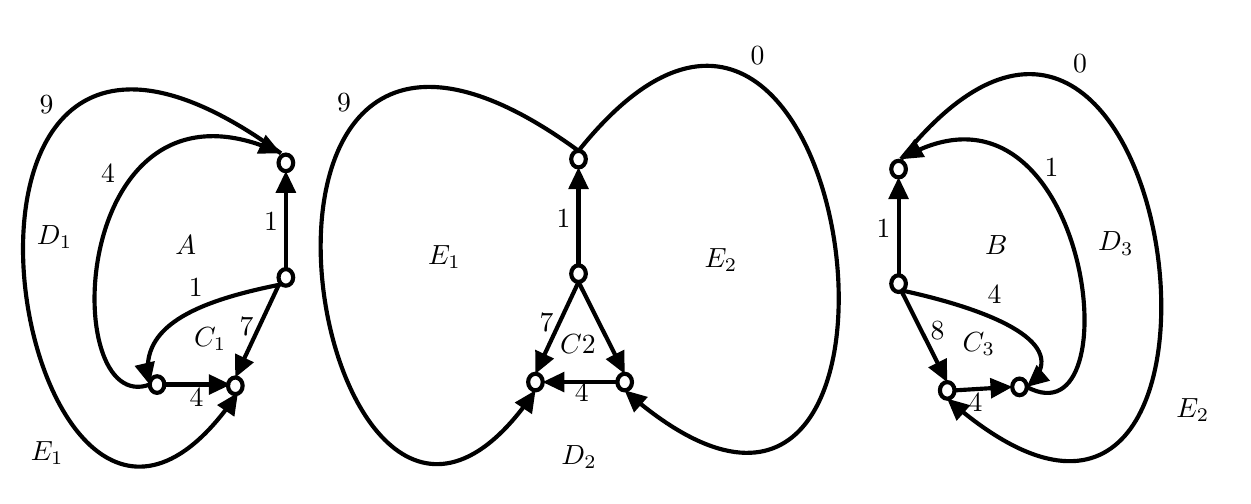
\begin{tikzpicture}[x=0.75pt,y=0.75pt,yscale=-0.9,xscale=0.9]
%uncomment if require: \path (0,498); %set diagram left start at 0, and has height of 498
\path[use as bounding box] (20,10) rectangle (660,250);
%Shape: Ellipse [id:dp012401419565516214] 
\draw  [color={rgb, 255:red, 0; green, 0; blue, 0 }  ,draw opacity=1 ][line width=1.5]  (310.98,80.38) .. controls (310.98,77.92) and (312.73,75.93) .. (314.89,75.93) .. controls (317.05,75.93) and (318.8,77.92) .. (318.8,80.38) .. controls (318.8,82.83) and (317.05,84.82) .. (314.89,84.82) .. controls (312.73,84.82) and (310.98,82.83) .. (310.98,80.38) -- cycle ;
%Shape: Ellipse [id:dp44563585877978507] 
\draw  [color={rgb, 255:red, 0; green, 0; blue, 0 }  ,draw opacity=1 ][line width=1.5]  (310.98,141.69) .. controls (310.98,139.23) and (312.73,137.24) .. (314.89,137.24) .. controls (317.05,137.24) and (318.8,139.23) .. (318.8,141.69) .. controls (318.8,144.14) and (317.05,146.13) .. (314.89,146.13) .. controls (312.73,146.13) and (310.98,144.14) .. (310.98,141.69) -- cycle ;
%Shape: Ellipse [id:dp8232398640866994] 
\draw  [color={rgb, 255:red, 0; green, 0; blue, 0 }  ,draw opacity=1 ][line width=1.5]  (287.92,199.72) .. controls (287.92,197.26) and (289.67,195.27) .. (291.83,195.27) .. controls (293.99,195.27) and (295.74,197.26) .. (295.74,199.72) .. controls (295.74,202.17) and (293.99,204.16) .. (291.83,204.16) .. controls (289.67,204.16) and (287.92,202.17) .. (287.92,199.72) -- cycle ;
%Shape: Ellipse [id:dp43325876938835506] 
\draw  [color={rgb, 255:red, 0; green, 0; blue, 0 }  ,draw opacity=1 ][line width=1.5]  (335.68,199.72) .. controls (335.68,197.26) and (337.44,195.27) .. (339.6,195.27) .. controls (341.76,195.27) and (343.51,197.26) .. (343.51,199.72) .. controls (343.51,202.17) and (341.76,204.16) .. (339.6,204.16) .. controls (337.44,204.16) and (335.68,202.17) .. (335.68,199.72) -- cycle ;
%Straight Lines [id:da24688497873734994] 
\draw [color={rgb, 255:red, 0; green, 0; blue, 0 }  ,draw opacity=1 ][line width=1.5]    (299.74,199.72) -- (335.68,199.72) ;
\draw [shift={(295.74,199.72)}, rotate = 0] [fill={rgb, 255:red, 0; green, 0; blue, 0 }  ,fill opacity=1 ][line width=0.08]  [draw opacity=0] (11.61,-5.58) -- (0,0) -- (11.61,5.58) -- cycle    ;
%Straight Lines [id:da9029001126541812] 
\draw [color={rgb, 255:red, 0; green, 0; blue, 0 }  ,draw opacity=1 ][line width=1.5]    (314.89,137.24) -- (314.89,88.82) ;
\draw [shift={(314.89,84.82)}, rotate = 90] [fill={rgb, 255:red, 0; green, 0; blue, 0 }  ,fill opacity=1 ][line width=0.08]  [draw opacity=0] (11.61,-5.58) -- (0,0) -- (11.61,5.58) -- cycle    ;
%Straight Lines [id:da22131359142153095] 
\draw [color={rgb, 255:red, 0; green, 0; blue, 0 }  ,draw opacity=1 ][line width=1.5]    (314.89,146.13) -- (293.53,191.65) ;
\draw [shift={(291.83,195.27)}, rotate = 295.14] [fill={rgb, 255:red, 0; green, 0; blue, 0 }  ,fill opacity=1 ][line width=0.08]  [draw opacity=0] (11.61,-5.58) -- (0,0) -- (11.61,5.58) -- cycle    ;
%Straight Lines [id:da6387841366636108] 
\draw [color={rgb, 255:red, 0; green, 0; blue, 0 }  ,draw opacity=1 ][line width=1.5]    (314.89,146.13) -- (337.8,191.7) ;
\draw [shift={(339.6,195.27)}, rotate = 243.31] [fill={rgb, 255:red, 0; green, 0; blue, 0 }  ,fill opacity=1 ][line width=0.08]  [draw opacity=0] (11.61,-5.58) -- (0,0) -- (11.61,5.58) -- cycle    ;
%Curve Lines [id:da15562696066606252] 
\draw [line width=1.5]    (314.89,75.93) .. controls (97.2,-83.01) and (174.77,372.56) .. (290.09,206.71) ;
\draw [shift={(291.83,204.16)}, rotate = 123.91] [fill={rgb, 255:red, 0; green, 0; blue, 0 }  ][line width=0.08]  [draw opacity=0] (11.61,-5.58) -- (0,0) -- (11.61,5.58) -- cycle    ;
%Curve Lines [id:da37566750523718095] 
\draw [line width=1.5]    (314.89,75.93) .. controls (466.51,-113.62) and (520.64,359.85) .. (342.3,206.52) ;
\draw [shift={(339.6,204.16)}, rotate = 41.47] [fill={rgb, 255:red, 0; green, 0; blue, 0 }  ][line width=0.08]  [draw opacity=0] (11.61,-5.58) -- (0,0) -- (11.61,5.58) -- cycle    ;
%Shape: Ellipse [id:dp2127358898052878] 
\draw  [color={rgb, 255:red, 0; green, 0; blue, 0 }  ,draw opacity=1 ][line width=1.5]  (85.35,201.05) .. controls (85.35,198.6) and (87.1,196.61) .. (89.26,196.61) .. controls (91.42,196.61) and (93.17,198.6) .. (93.17,201.05) .. controls (93.17,203.51) and (91.42,205.5) .. (89.26,205.5) .. controls (87.1,205.5) and (85.35,203.51) .. (85.35,201.05) -- cycle ;
%Curve Lines [id:da6892910775973166] 
\draw [color={rgb, 255:red, 0; green, 0; blue, 0 }  ,draw opacity=1 ][line width=1.5]    (84.57,196.85) .. controls (81.15,170.86) and (107.05,157.02) .. (155.56,147.47) ;
\draw [shift={(85.35,201.05)}, rotate = 256.57] [fill={rgb, 255:red, 0; green, 0; blue, 0 }  ,fill opacity=1 ][line width=0.08]  [draw opacity=0] (11.61,-5.58) -- (0,0) -- (11.61,5.58) -- cycle    ;
%Curve Lines [id:da5288751216338294] 
\draw [color={rgb, 255:red, 0; green, 0; blue, 0 }  ,draw opacity=1 ][line width=1.5]    (85.35,201.05) .. controls (36.23,219.12) and (41.79,28.03) .. (152.18,75.75) ;
\draw [shift={(155.56,77.27)}, rotate = 205.05] [fill={rgb, 255:red, 0; green, 0; blue, 0 }  ,fill opacity=1 ][line width=0.08]  [draw opacity=0] (11.61,-5.58) -- (0,0) -- (11.61,5.58) -- cycle    ;
%Straight Lines [id:da24276479087471536] 
\draw [color={rgb, 255:red, 0; green, 0; blue, 0 }  ,draw opacity=1 ][line width=1.5]    (93.17,201.05) -- (124.59,201.05) ;
\draw [shift={(128.59,201.05)}, rotate = 180] [fill={rgb, 255:red, 0; green, 0; blue, 0 }  ,fill opacity=1 ][line width=0.08]  [draw opacity=0] (11.61,-5.58) -- (0,0) -- (11.61,5.58) -- cycle    ;
%Curve Lines [id:da32788257215994565] 
\draw [line width=1.5]    (155.56,77.27) .. controls (-62.14,-81.67) and (15.44,373.9) .. (130.76,208.05) ;
\draw [shift={(132.5,205.5)}, rotate = 123.91] [fill={rgb, 255:red, 0; green, 0; blue, 0 }  ][line width=0.08]  [draw opacity=0] (11.61,-5.58) -- (0,0) -- (11.61,5.58) -- cycle    ;
%Shape: Ellipse [id:dp4018621662081351] 
\draw  [color={rgb, 255:red, 0; green, 0; blue, 0 }  ,draw opacity=1 ][line width=1.5]  (127.25,201.72) .. controls (127.25,199.26) and (129,197.27) .. (131.16,197.27) .. controls (133.32,197.27) and (135.08,199.26) .. (135.08,201.72) .. controls (135.08,204.17) and (133.32,206.16) .. (131.16,206.16) .. controls (129,206.16) and (127.25,204.17) .. (127.25,201.72) -- cycle ;
%Straight Lines [id:da06341837878705825] 
\draw [color={rgb, 255:red, 0; green, 0; blue, 0 }  ,draw opacity=1 ][line width=1.5]    (154.22,148.13) -- (132.86,193.65) ;
\draw [shift={(131.16,197.27)}, rotate = 295.14] [fill={rgb, 255:red, 0; green, 0; blue, 0 }  ,fill opacity=1 ][line width=0.08]  [draw opacity=0] (11.61,-5.58) -- (0,0) -- (11.61,5.58) -- cycle    ;
%Shape: Ellipse [id:dp38906306008016145] 
\draw  [color={rgb, 255:red, 0; green, 0; blue, 0 }  ,draw opacity=1 ][line width=1.5]  (154.31,82.38) .. controls (154.31,79.92) and (156.06,77.93) .. (158.22,77.93) .. controls (160.38,77.93) and (162.14,79.92) .. (162.14,82.38) .. controls (162.14,84.83) and (160.38,86.82) .. (158.22,86.82) .. controls (156.06,86.82) and (154.31,84.83) .. (154.31,82.38) -- cycle ;
%Shape: Ellipse [id:dp08743735948745213] 
\draw  [color={rgb, 255:red, 0; green, 0; blue, 0 }  ,draw opacity=1 ][line width=1.5]  (154.31,143.69) .. controls (154.31,141.23) and (156.06,139.24) .. (158.22,139.24) .. controls (160.38,139.24) and (162.14,141.23) .. (162.14,143.69) .. controls (162.14,146.14) and (160.38,148.13) .. (158.22,148.13) .. controls (156.06,148.13) and (154.31,146.14) .. (154.31,143.69) -- cycle ;
%Straight Lines [id:da6699514353142748] 
\draw [color={rgb, 255:red, 0; green, 0; blue, 0 }  ,draw opacity=1 ][line width=1.5]    (158.22,139.24) -- (158.22,90.82) ;
\draw [shift={(158.22,86.82)}, rotate = 90] [fill={rgb, 255:red, 0; green, 0; blue, 0 }  ,fill opacity=1 ][line width=0.08]  [draw opacity=0] (11.61,-5.58) -- (0,0) -- (11.61,5.58) -- cycle    ;
%Shape: Ellipse [id:dp8050348596658142] 
\draw  [color={rgb, 255:red, 0; green, 0; blue, 0 }  ,draw opacity=1 ][line width=1.5]  (547.06,202.3) .. controls (547.06,199.84) and (548.81,197.85) .. (550.97,197.85) .. controls (553.13,197.85) and (554.88,199.84) .. (554.88,202.3) .. controls (554.88,204.75) and (553.13,206.75) .. (550.97,206.75) .. controls (548.81,206.75) and (547.06,204.75) .. (547.06,202.3) -- cycle ;
%Shape: Ellipse [id:dp4814843770420125] 
\draw  [color={rgb, 255:red, 0; green, 0; blue, 0 }  ,draw opacity=1 ][line width=1.5]  (508.35,204.17) .. controls (508.35,201.72) and (510.1,199.73) .. (512.26,199.73) .. controls (514.42,199.73) and (516.18,201.72) .. (516.18,204.17) .. controls (516.18,206.63) and (514.42,208.62) .. (512.26,208.62) .. controls (510.1,208.62) and (508.35,206.63) .. (508.35,204.17) -- cycle ;
%Curve Lines [id:da6756687162833178] 
\draw [color={rgb, 255:red, 0; green, 0; blue, 0 }  ,draw opacity=1 ][line width=1.5]    (557.85,199.47) .. controls (576.23,179.57) and (540.25,161.98) .. (487.56,150.59) ;
\draw [shift={(554.88,202.3)}, rotate = 319.56] [fill={rgb, 255:red, 0; green, 0; blue, 0 }  ,fill opacity=1 ][line width=0.08]  [draw opacity=0] (11.61,-5.58) -- (0,0) -- (11.61,5.58) -- cycle    ;
%Curve Lines [id:da3167596918642579] 
\draw [color={rgb, 255:red, 0; green, 0; blue, 0 }  ,draw opacity=1 ][line width=1.5]    (554.88,202.3) .. controls (612.57,233.81) and (588.52,24.96) .. (490.55,78.68) ;
\draw [shift={(487.56,80.38)}, rotate = 329.29] [fill={rgb, 255:red, 0; green, 0; blue, 0 }  ,fill opacity=1 ][line width=0.08]  [draw opacity=0] (11.61,-5.58) -- (0,0) -- (11.61,5.58) -- cycle    ;
%Straight Lines [id:da5914875377963786] 
\draw [color={rgb, 255:red, 0; green, 0; blue, 0 }  ,draw opacity=1 ][line width=1.5]    (516.18,204.17) -- (543.07,202.54) ;
\draw [shift={(547.06,202.3)}, rotate = 176.53] [fill={rgb, 255:red, 0; green, 0; blue, 0 }  ,fill opacity=1 ][line width=0.08]  [draw opacity=0] (11.61,-5.58) -- (0,0) -- (11.61,5.58) -- cycle    ;
%Straight Lines [id:da07161147378506905] 
\draw [color={rgb, 255:red, 0; green, 0; blue, 0 }  ,draw opacity=1 ][line width=1.5]    (487.56,150.59) -- (510.47,196.15) ;
\draw [shift={(512.26,199.73)}, rotate = 243.31] [fill={rgb, 255:red, 0; green, 0; blue, 0 }  ,fill opacity=1 ][line width=0.08]  [draw opacity=0] (11.61,-5.58) -- (0,0) -- (11.61,5.58) -- cycle    ;
%Curve Lines [id:da5080118287083738] 
\draw [line width=1.5]    (487.56,80.38) .. controls (639.17,-109.17) and (693.31,364.3) .. (514.97,210.98) ;
\draw [shift={(512.26,208.62)}, rotate = 41.47] [fill={rgb, 255:red, 0; green, 0; blue, 0 }  ][line width=0.08]  [draw opacity=0] (11.61,-5.58) -- (0,0) -- (11.61,5.58) -- cycle    ;
%Shape: Ellipse [id:dp8095971328672295] 
\draw  [color={rgb, 255:red, 0; green, 0; blue, 0 }  ,draw opacity=1 ][line width=1.5]  (482.31,85.71) .. controls (482.31,83.26) and (484.06,81.27) .. (486.22,81.27) .. controls (488.38,81.27) and (490.14,83.26) .. (490.14,85.71) .. controls (490.14,88.17) and (488.38,90.16) .. (486.22,90.16) .. controls (484.06,90.16) and (482.31,88.17) .. (482.31,85.71) -- cycle ;
%Shape: Ellipse [id:dp915558520007347] 
\draw  [color={rgb, 255:red, 0; green, 0; blue, 0 }  ,draw opacity=1 ][line width=1.5]  (482.31,147.02) .. controls (482.31,144.56) and (484.06,142.57) .. (486.22,142.57) .. controls (488.38,142.57) and (490.14,144.56) .. (490.14,147.02) .. controls (490.14,149.47) and (488.38,151.47) .. (486.22,151.47) .. controls (484.06,151.47) and (482.31,149.47) .. (482.31,147.02) -- cycle ;
%Straight Lines [id:da8569739762561568] 
\draw [color={rgb, 255:red, 0; green, 0; blue, 0 }  ,draw opacity=1 ][line width=1.5]    (486.22,142.57) -- (486.22,94.16) ;
\draw [shift={(486.22,90.16)}, rotate = 90] [fill={rgb, 255:red, 0; green, 0; blue, 0 }  ,fill opacity=1 ][line width=0.08]  [draw opacity=0] (11.61,-5.58) -- (0,0) -- (11.61,5.58) -- cycle    ;

% Text Node
\draw (311.27,198.94) node [anchor=north west][inner sep=0.75pt]    {$4$};
% Text Node
\draw (301.54,105.56) node [anchor=north west][inner sep=0.75pt]    {$1$};
% Text Node
\draw (303.43,172.5) node [anchor=north west][inner sep=0.75pt]    {$C2$};
% Text Node
\draw (304.1,231.81) node [anchor=north west][inner sep=0.75pt]    {$D_{2}$};
% Text Node
\draw (184.03,43.64) node [anchor=north west][inner sep=0.75pt]    {$9$};
% Text Node
\draw (405.37,18.28) node [anchor=north west][inner sep=0.75pt]    {$0$};
% Text Node
\draw (292.43,161.58) node [anchor=north west][inner sep=0.75pt]    {$7$};
% Text Node
\draw (97.44,119.41) node [anchor=north west][inner sep=0.75pt]    {$A$};
% Text Node
\draw (23.28,114.24) node [anchor=north west][inner sep=0.75pt]    {$D_{1}$};
% Text Node
\draw (104.58,142.94) node [anchor=north west][inner sep=0.75pt]    {$1$};
% Text Node
\draw (57.66,81.61) node [anchor=north west][inner sep=0.75pt]    {$4$};
% Text Node
\draw (105.02,201.78) node [anchor=north west][inner sep=0.75pt]    {$4$};
% Text Node
\draw (107.45,168.75) node [anchor=north west][inner sep=0.75pt]    {$C_{1}$};
% Text Node
\draw (24.7,44.97) node [anchor=north west][inner sep=0.75pt]    {$9$};
% Text Node
\draw (131.76,163.58) node [anchor=north west][inner sep=0.75pt]    {$7$};
% Text Node
\draw (144.87,107.56) node [anchor=north west][inner sep=0.75pt]    {$1$};
% Text Node
\draw (633.33,207.07) node [anchor=north west][inner sep=0.75pt]    {$E_{2}$};
% Text Node
\draw (380.67,126.4) node [anchor=north west][inner sep=0.75pt]    {$E_{2}$};
% Text Node
\draw (530.86,119.53) node [anchor=north west][inner sep=0.75pt]    {$B$};
% Text Node
\draw (562.73,78.22) node [anchor=north west][inner sep=0.75pt]    {$1$};
% Text Node
\draw (532.19,146.31) node [anchor=north west][inner sep=0.75pt]    {$4$};
% Text Node
\draw (522.01,204.4) node [anchor=north west][inner sep=0.75pt]    {$4$};
% Text Node
\draw (518.91,171.59) node [anchor=north west][inner sep=0.75pt]    {$C_{3}$};
% Text Node
\draw (591.4,117.74) node [anchor=north west][inner sep=0.75pt]    {$D_{3}$};
% Text Node
\draw (578.03,22.73) node [anchor=north west][inner sep=0.75pt]    {$0$};
% Text Node
\draw (501.7,165.47) node [anchor=north west][inner sep=0.75pt]    {$8$};
% Text Node
\draw (472.87,110.89) node [anchor=north west][inner sep=0.75pt]    {$1$};
% Text Node
\draw (232.67,125.07) node [anchor=north west][inner sep=0.75pt]    {$E_{1}$};
% Text Node
\draw (20,229.73) node [anchor=north west][inner sep=0.75pt]    {$E_{1}$};


\end{tikzpicture}
    \caption{Subdivisión en tres tetraedros del poliedro de arriba}
\end{figure}
De una manera similar podemos hacer una subdivisión del poliedro de abajo como se muestra a continuación
\begin{figure}[H]
\centering
%!TEX root = ./main.tex




\tikzset{every picture/.style={line width=0.75pt}} %set default line width to 0.75pt        

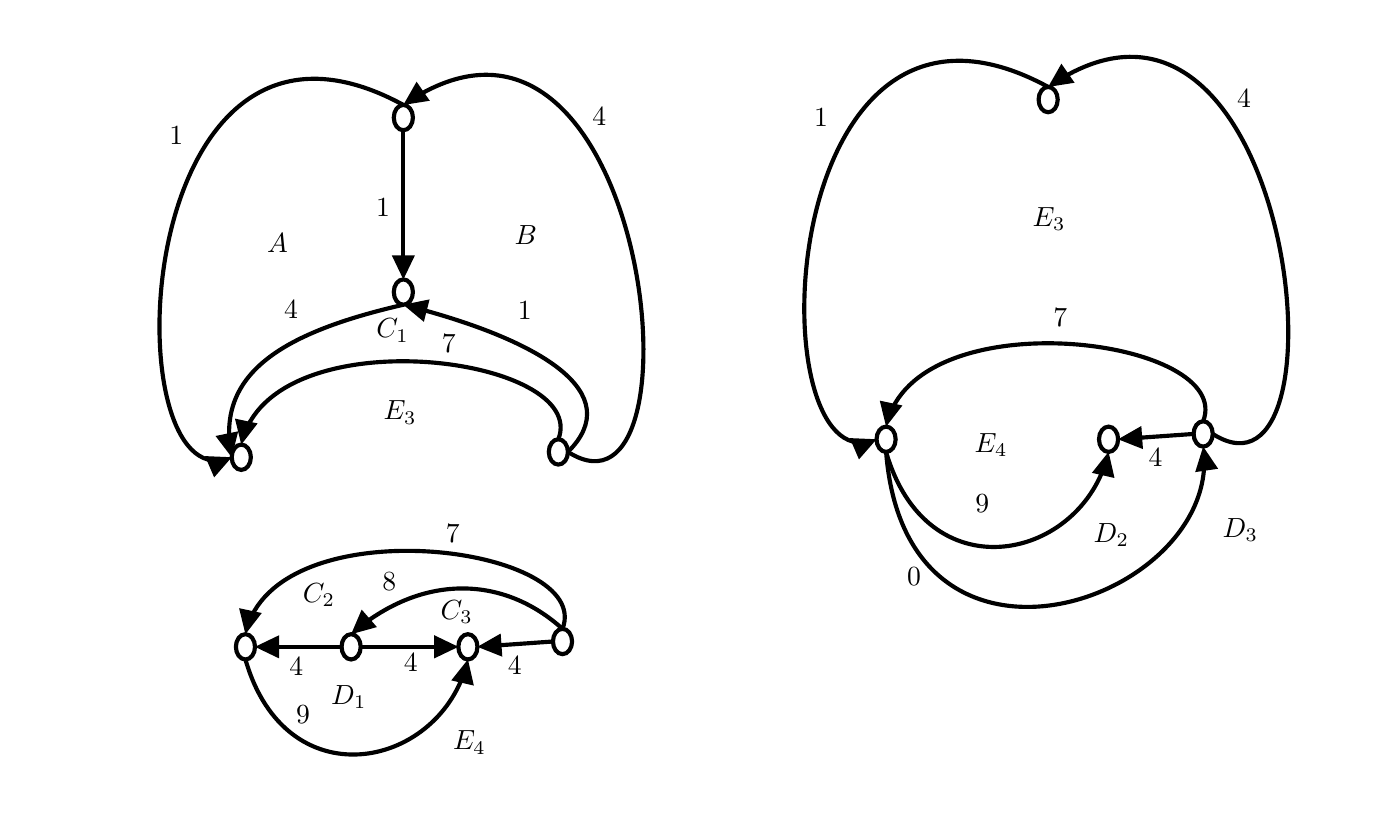
\begin{tikzpicture}[x=0.75pt,y=0.75pt,yscale=-1,xscale=1]
%uncomment if require: \path (0,498); %set diagram left start at 0, and has height of 498
\path[use as bounding box] (20,10) rectangle (660,380);
%Shape: Ellipse [id:dp35589263376995484] 
\draw  [color={rgb, 255:red, 0; green, 0; blue, 0 }  ,draw opacity=1 ][line width=1.5]  (507.06,44.65) .. controls (507.06,41.28) and (509.12,38.55) .. (511.67,38.55) .. controls (514.21,38.55) and (516.27,41.28) .. (516.27,44.65) .. controls (516.27,48.02) and (514.21,50.75) .. (511.67,50.75) .. controls (509.12,50.75) and (507.06,48.02) .. (507.06,44.65) -- cycle ;
%Shape: Ellipse [id:dp5273685537709042] 
\draw  [color={rgb, 255:red, 0; green, 0; blue, 0 }  ,draw opacity=1 ][line width=1.5]  (428.98,208.3) .. controls (428.98,204.94) and (431.04,202.21) .. (433.59,202.21) .. controls (436.13,202.21) and (438.19,204.94) .. (438.19,208.3) .. controls (438.19,211.67) and (436.13,214.4) .. (433.59,214.4) .. controls (431.04,214.4) and (428.98,211.67) .. (428.98,208.3) -- cycle ;
%Shape: Ellipse [id:dp9933087224039621] 
\draw  [color={rgb, 255:red, 0; green, 0; blue, 0 }  ,draw opacity=1 ][line width=1.5]  (581.74,205.74) .. controls (581.74,202.37) and (583.8,199.64) .. (586.35,199.64) .. controls (588.89,199.64) and (590.96,202.37) .. (590.96,205.74) .. controls (590.96,209.1) and (588.89,211.83) .. (586.35,211.83) .. controls (583.8,211.83) and (581.74,209.1) .. (581.74,205.74) -- cycle ;
%Shape: Ellipse [id:dp4223187867652599] 
\draw  [color={rgb, 255:red, 0; green, 0; blue, 0 }  ,draw opacity=1 ][line width=1.5]  (536.16,208.3) .. controls (536.16,204.94) and (538.22,202.21) .. (540.76,202.21) .. controls (543.31,202.21) and (545.37,204.94) .. (545.37,208.3) .. controls (545.37,211.67) and (543.31,214.4) .. (540.76,214.4) .. controls (538.22,214.4) and (536.16,211.67) .. (536.16,208.3) -- cycle ;
%Curve Lines [id:da32707407117974907] 
\draw [color={rgb, 255:red, 0; green, 0; blue, 0 }  ,draw opacity=1 ][line width=1.5]    (590.96,205.74) .. controls (659.24,249.16) and (630.29,-40.35) .. (513.43,37.36) ;
\draw [shift={(511.67,38.55)}, rotate = 325.34] [fill={rgb, 255:red, 0; green, 0; blue, 0 }  ,fill opacity=1 ][line width=0.08]  [draw opacity=0] (11.61,-5.58) -- (0,0) -- (11.61,5.58) -- cycle    ;
%Curve Lines [id:da7020868150054066] 
\draw [color={rgb, 255:red, 0; green, 0; blue, 0 }  ,draw opacity=1 ][line width=1.5]    (424.72,209.64) .. controls (370.98,220.16) and (381.16,-32.47) .. (511.67,38.55) ;
\draw [shift={(428.98,208.3)}, rotate = 156.81] [fill={rgb, 255:red, 0; green, 0; blue, 0 }  ,fill opacity=1 ][line width=0.08]  [draw opacity=0] (11.61,-5.58) -- (0,0) -- (11.61,5.58) -- cycle    ;
%Straight Lines [id:da6734901748040498] 
\draw [color={rgb, 255:red, 0; green, 0; blue, 0 }  ,draw opacity=1 ][line width=1.5]    (549.36,208.02) -- (581.74,205.74) ;
\draw [shift={(545.37,208.3)}, rotate = 355.96] [fill={rgb, 255:red, 0; green, 0; blue, 0 }  ,fill opacity=1 ][line width=0.08]  [draw opacity=0] (11.61,-5.58) -- (0,0) -- (11.61,5.58) -- cycle    ;
%Curve Lines [id:da03703637046060837] 
\draw [line width=1.5]    (586.35,199.64) .. controls (601.62,160.02) and (453,140.46) .. (434.55,198.55) ;
\draw [shift={(433.59,202.21)}, rotate = 281.99] [fill={rgb, 255:red, 0; green, 0; blue, 0 }  ][line width=0.08]  [draw opacity=0] (11.61,-5.58) -- (0,0) -- (11.61,5.58) -- cycle    ;
%Curve Lines [id:da798612936169141] 
\draw [line width=1.5]    (433.59,214.4) .. controls (453.03,281.98) and (525.13,267.42) .. (539.75,218.25) ;
\draw [shift={(540.76,214.4)}, rotate = 102.83] [fill={rgb, 255:red, 0; green, 0; blue, 0 }  ][line width=0.08]  [draw opacity=0] (11.61,-5.58) -- (0,0) -- (11.61,5.58) -- cycle    ;
%Curve Lines [id:da8888761441506123] 
\draw [line width=1.5]    (433.59,214.4) .. controls (443.17,338.24) and (592.39,286.2) .. (586.72,215.09) ;
\draw [shift={(586.35,211.83)}, rotate = 81.69] [fill={rgb, 255:red, 0; green, 0; blue, 0 }  ][line width=0.08]  [draw opacity=0] (11.61,-5.58) -- (0,0) -- (11.61,5.58) -- cycle    ;
%Shape: Ellipse [id:dp8150638560518382] 
\draw  [color={rgb, 255:red, 0; green, 0; blue, 0 }  ,draw opacity=1 ][line width=1.5]  (196.39,53.32) .. controls (196.39,49.95) and (198.45,47.22) .. (201,47.22) .. controls (203.54,47.22) and (205.61,49.95) .. (205.61,53.32) .. controls (205.61,56.69) and (203.54,59.41) .. (201,59.41) .. controls (198.45,59.41) and (196.39,56.69) .. (196.39,53.32) -- cycle ;
%Shape: Ellipse [id:dp07405350698131474] 
\draw  [color={rgb, 255:red, 0; green, 0; blue, 0 }  ,draw opacity=1 ][line width=1.5]  (196.39,137.39) .. controls (196.39,134.02) and (198.45,131.29) .. (201,131.29) .. controls (203.54,131.29) and (205.61,134.02) .. (205.61,137.39) .. controls (205.61,140.76) and (203.54,143.49) .. (201,143.49) .. controls (198.45,143.49) and (196.39,140.76) .. (196.39,137.39) -- cycle ;
%Curve Lines [id:da5729143394323514] 
\draw [color={rgb, 255:red, 0; green, 0; blue, 0 }  ,draw opacity=1 ][line width=1.5]    (117.61,212.9) .. controls (112.41,176.16) and (142.97,156.8) .. (201,143.49) ;
\draw [shift={(118.31,216.97)}, rotate = 258.41] [fill={rgb, 255:red, 0; green, 0; blue, 0 }  ,fill opacity=1 ][line width=0.08]  [draw opacity=0] (11.61,-5.58) -- (0,0) -- (11.61,5.58) -- cycle    ;
%Curve Lines [id:da985022859832252] 
\draw [color={rgb, 255:red, 0; green, 0; blue, 0 }  ,draw opacity=1 ][line width=1.5]    (280.29,214.4) .. controls (308.81,186.1) and (267.69,160.88) .. (204.87,144.48) ;
\draw [shift={(201,143.49)}, rotate = 14.13] [fill={rgb, 255:red, 0; green, 0; blue, 0 }  ,fill opacity=1 ][line width=0.08]  [draw opacity=0] (11.61,-5.58) -- (0,0) -- (11.61,5.58) -- cycle    ;
%Curve Lines [id:da42144751436003447] 
\draw [color={rgb, 255:red, 0; green, 0; blue, 0 }  ,draw opacity=1 ][line width=1.5]    (280.29,214.4) .. controls (348.57,257.82) and (319.62,-31.69) .. (202.77,46.02) ;
\draw [shift={(201,47.22)}, rotate = 325.34] [fill={rgb, 255:red, 0; green, 0; blue, 0 }  ,fill opacity=1 ][line width=0.08]  [draw opacity=0] (11.61,-5.58) -- (0,0) -- (11.61,5.58) -- cycle    ;
%Curve Lines [id:da7830144424190421] 
\draw [color={rgb, 255:red, 0; green, 0; blue, 0 }  ,draw opacity=1 ][line width=1.5]    (114.05,218.31) .. controls (60.32,228.83) and (70.5,-23.8) .. (201,47.22) ;
\draw [shift={(118.31,216.97)}, rotate = 156.81] [fill={rgb, 255:red, 0; green, 0; blue, 0 }  ,fill opacity=1 ][line width=0.08]  [draw opacity=0] (11.61,-5.58) -- (0,0) -- (11.61,5.58) -- cycle    ;
%Straight Lines [id:da11394903068946982] 
\draw [color={rgb, 255:red, 0; green, 0; blue, 0 }  ,draw opacity=1 ][line width=1.5]    (201,127.29) -- (201,59.41) ;
\draw [shift={(201,131.29)}, rotate = 270] [fill={rgb, 255:red, 0; green, 0; blue, 0 }  ,fill opacity=1 ][line width=0.08]  [draw opacity=0] (11.61,-5.58) -- (0,0) -- (11.61,5.58) -- cycle    ;
%Curve Lines [id:da9079411866287189] 
\draw [line width=1.5]    (275.68,208.31) .. controls (290.96,168.68) and (142.33,149.13) .. (123.88,207.22) ;
\draw [shift={(122.92,210.87)}, rotate = 281.99] [fill={rgb, 255:red, 0; green, 0; blue, 0 }  ][line width=0.08]  [draw opacity=0] (11.61,-5.58) -- (0,0) -- (11.61,5.58) -- cycle    ;
%Shape: Ellipse [id:dp9797878316847205] 
\draw  [color={rgb, 255:red, 0; green, 0; blue, 0 }  ,draw opacity=1 ][line width=1.5]  (271.08,214.4) .. controls (271.08,211.03) and (273.14,208.31) .. (275.68,208.31) .. controls (278.23,208.31) and (280.29,211.03) .. (280.29,214.4) .. controls (280.29,217.77) and (278.23,220.5) .. (275.68,220.5) .. controls (273.14,220.5) and (271.08,217.77) .. (271.08,214.4) -- cycle ;
%Shape: Ellipse [id:dp11924297827138353] 
\draw  [color={rgb, 255:red, 0; green, 0; blue, 0 }  ,draw opacity=1 ][line width=1.5]  (120.31,308.3) .. controls (120.31,304.94) and (122.38,302.21) .. (124.92,302.21) .. controls (127.46,302.21) and (129.53,304.94) .. (129.53,308.3) .. controls (129.53,311.67) and (127.46,314.4) .. (124.92,314.4) .. controls (122.38,314.4) and (120.31,311.67) .. (120.31,308.3) -- cycle ;
%Shape: Ellipse [id:dp18019428491254885] 
\draw  [color={rgb, 255:red, 0; green, 0; blue, 0 }  ,draw opacity=1 ][line width=1.5]  (118.31,216.97) .. controls (118.31,213.6) and (120.38,210.87) .. (122.92,210.87) .. controls (125.46,210.87) and (127.53,213.6) .. (127.53,216.97) .. controls (127.53,220.34) and (125.46,223.07) .. (122.92,223.07) .. controls (120.38,223.07) and (118.31,220.34) .. (118.31,216.97) -- cycle ;
%Shape: Ellipse [id:dp2447839509836378] 
\draw  [color={rgb, 255:red, 0; green, 0; blue, 0 }  ,draw opacity=1 ][line width=1.5]  (171.23,308.3) .. controls (171.23,304.94) and (173.3,302.21) .. (175.84,302.21) .. controls (178.39,302.21) and (180.45,304.94) .. (180.45,308.3) .. controls (180.45,311.67) and (178.39,314.4) .. (175.84,314.4) .. controls (173.3,314.4) and (171.23,311.67) .. (171.23,308.3) -- cycle ;
%Shape: Ellipse [id:dp33013962263442154] 
\draw  [color={rgb, 255:red, 0; green, 0; blue, 0 }  ,draw opacity=1 ][line width=1.5]  (227.49,308.3) .. controls (227.49,304.94) and (229.55,302.21) .. (232.1,302.21) .. controls (234.64,302.21) and (236.7,304.94) .. (236.7,308.3) .. controls (236.7,311.67) and (234.64,314.4) .. (232.1,314.4) .. controls (229.55,314.4) and (227.49,311.67) .. (227.49,308.3) -- cycle ;
%Straight Lines [id:da31396117550667135] 
\draw [color={rgb, 255:red, 0; green, 0; blue, 0 }  ,draw opacity=1 ][line width=1.5]    (133.53,308.3) -- (171.23,308.3) ;
\draw [shift={(129.53,308.3)}, rotate = 0] [fill={rgb, 255:red, 0; green, 0; blue, 0 }  ,fill opacity=1 ][line width=0.08]  [draw opacity=0] (11.61,-5.58) -- (0,0) -- (11.61,5.58) -- cycle    ;
%Straight Lines [id:da6005265572468635] 
\draw [color={rgb, 255:red, 0; green, 0; blue, 0 }  ,draw opacity=1 ][line width=1.5]    (180.45,308.3) -- (223.49,308.3) ;
\draw [shift={(227.49,308.3)}, rotate = 180] [fill={rgb, 255:red, 0; green, 0; blue, 0 }  ,fill opacity=1 ][line width=0.08]  [draw opacity=0] (11.61,-5.58) -- (0,0) -- (11.61,5.58) -- cycle    ;
%Straight Lines [id:da1808031690077344] 
\draw [color={rgb, 255:red, 0; green, 0; blue, 0 }  ,draw opacity=1 ][line width=1.5]    (240.69,308.02) -- (273.08,305.74) ;
\draw [shift={(236.7,308.3)}, rotate = 355.96] [fill={rgb, 255:red, 0; green, 0; blue, 0 }  ,fill opacity=1 ][line width=0.08]  [draw opacity=0] (11.61,-5.58) -- (0,0) -- (11.61,5.58) -- cycle    ;
%Curve Lines [id:da3357677157773651] 
\draw [line width=1.5]    (277.68,299.64) .. controls (292.96,260.02) and (144.33,240.46) .. (125.88,298.55) ;
\draw [shift={(124.92,302.21)}, rotate = 281.99] [fill={rgb, 255:red, 0; green, 0; blue, 0 }  ][line width=0.08]  [draw opacity=0] (11.61,-5.58) -- (0,0) -- (11.61,5.58) -- cycle    ;
%Curve Lines [id:da670250481056926] 
\draw [line width=1.5]    (179.35,299.27) .. controls (211.8,273.31) and (249.51,274.2) .. (277.68,299.64) ;
\draw [shift={(175.84,302.21)}, rotate = 318.94] [fill={rgb, 255:red, 0; green, 0; blue, 0 }  ][line width=0.08]  [draw opacity=0] (11.61,-5.58) -- (0,0) -- (11.61,5.58) -- cycle    ;
%Curve Lines [id:da1585249402391844] 
\draw [line width=1.5]    (124.92,314.4) .. controls (144.36,381.98) and (216.47,367.42) .. (231.09,318.25) ;
\draw [shift={(232.1,314.4)}, rotate = 102.83] [fill={rgb, 255:red, 0; green, 0; blue, 0 }  ][line width=0.08]  [draw opacity=0] (11.61,-5.58) -- (0,0) -- (11.61,5.58) -- cycle    ;
%Shape: Ellipse [id:dp8849254018327529] 
\draw  [color={rgb, 255:red, 0; green, 0; blue, 0 }  ,draw opacity=1 ][line width=1.5]  (273.08,305.74) .. controls (273.08,302.37) and (275.14,299.64) .. (277.68,299.64) .. controls (280.23,299.64) and (282.29,302.37) .. (282.29,305.74) .. controls (282.29,309.1) and (280.23,311.83) .. (277.68,311.83) .. controls (275.14,311.83) and (273.08,309.1) .. (273.08,305.74) -- cycle ;

% Text Node
\draw (601.26,38.41) node [anchor=north west][inner sep=0.75pt]    {$4$};
% Text Node
\draw (397.44,47.33) node [anchor=north west][inner sep=0.75pt]    {$1$};
% Text Node
\draw (558.52,211.43) node [anchor=north west][inner sep=0.75pt]    {$4$};
% Text Node
\draw (532.09,247.38) node [anchor=north west][inner sep=0.75pt]    {$D_{2}$};
% Text Node
\draw (594.24,244.82) node [anchor=north west][inner sep=0.75pt]    {$D_{3}$};
% Text Node
\draw (442.27,268.73) node [anchor=north west][inner sep=0.75pt]    {$0$};
% Text Node
\draw (133.88,107.84) node [anchor=north west][inner sep=0.75pt]    {$A$};
% Text Node
\draw (253.06,103.72) node [anchor=north west][inner sep=0.75pt]    {$B$};
% Text Node
\draw (290.6,47.07) node [anchor=north west][inner sep=0.75pt]    {$4$};
% Text Node
\draw (142.03,140.11) node [anchor=north west][inner sep=0.75pt]    {$4$};
% Text Node
\draw (254.63,140.45) node [anchor=north west][inner sep=0.75pt]    {$1$};
% Text Node
\draw (86.77,56) node [anchor=north west][inner sep=0.75pt]    {$1$};
% Text Node
\draw (186.34,90.67) node [anchor=north west][inner sep=0.75pt]    {$1$};
% Text Node
\draw (186.56,148.89) node [anchor=north west][inner sep=0.75pt]    {$C_{1}$};
% Text Node
\draw (218.02,156.44) node [anchor=north west][inner sep=0.75pt]    {$7$};
% Text Node
\draw (190,188.4) node [anchor=north west][inner sep=0.75pt]    {$E_{3}$};
% Text Node
\draw (144.55,312.12) node [anchor=north west][inner sep=0.75pt]    {$4$};
% Text Node
\draw (199.81,310.06) node [anchor=north west][inner sep=0.75pt]    {$4$};
% Text Node
\draw (249.85,311.43) node [anchor=north west][inner sep=0.75pt]    {$4$};
% Text Node
\draw (217.5,284.38) node [anchor=north west][inner sep=0.75pt]    {$C_{3}$};
% Text Node
\draw (151.1,276.12) node [anchor=north west][inner sep=0.75pt]    {$C_{2}$};
% Text Node
\draw (220.02,247.77) node [anchor=north west][inner sep=0.75pt]    {$7$};
% Text Node
\draw (189.37,271.13) node [anchor=north west][inner sep=0.75pt]    {$8$};
% Text Node
\draw (164.69,325.59) node [anchor=north west][inner sep=0.75pt]    {$D_{1}$};
% Text Node
\draw (223.43,347.38) node [anchor=north west][inner sep=0.75pt]    {$E_{4}$};
% Text Node
\draw (147.8,335.38) node [anchor=north west][inner sep=0.75pt]    {$9$};
% Text Node
\draw (512.68,143.77) node [anchor=north west][inner sep=0.75pt]    {$7$};
% Text Node
\draw (502.67,95.07) node [anchor=north west][inner sep=0.75pt]    {$E_{3}$};
% Text Node
\draw (475.13,233.38) node [anchor=north west][inner sep=0.75pt]    {$9$};
% Text Node
\draw (474.76,204.05) node [anchor=north west][inner sep=0.75pt]    {$E_{4}$};


\end{tikzpicture}
    \caption{Subdivisión del poliedro de abajo}
\end{figure}
Observe particularmente que el poliedro de la derecha del todo no es exactamente un tetraedro, ya que la unión de las caras $E_4$ y $D_2$ forman un digono y no un cuadrilátero, como pasaría en un tetraedro, Por lo que si identificamos 0 con 7, cuando hacemos esto las caras $E_4$ y $D_2$ se identifican entre si, lo mismo ocurre con $E_3$ y $D_3$, por lo que esto no es otra cosa que el grafo de un triangulo sobre la 3-bola, por lo que en el pegado no tienen incidencia, así nuestra triangulación topológica ideal del complemento del nudo $6_1$ la podemos ver como el pegado de los siguientes 5 tetraedros todos vistos ahora desde afuera.
\begin{figure}[H]
\centering
%!TEX root = ./main.tex



\tikzset{every picture/.style={line width=0.75pt}} %set default line width to 0.75pt        

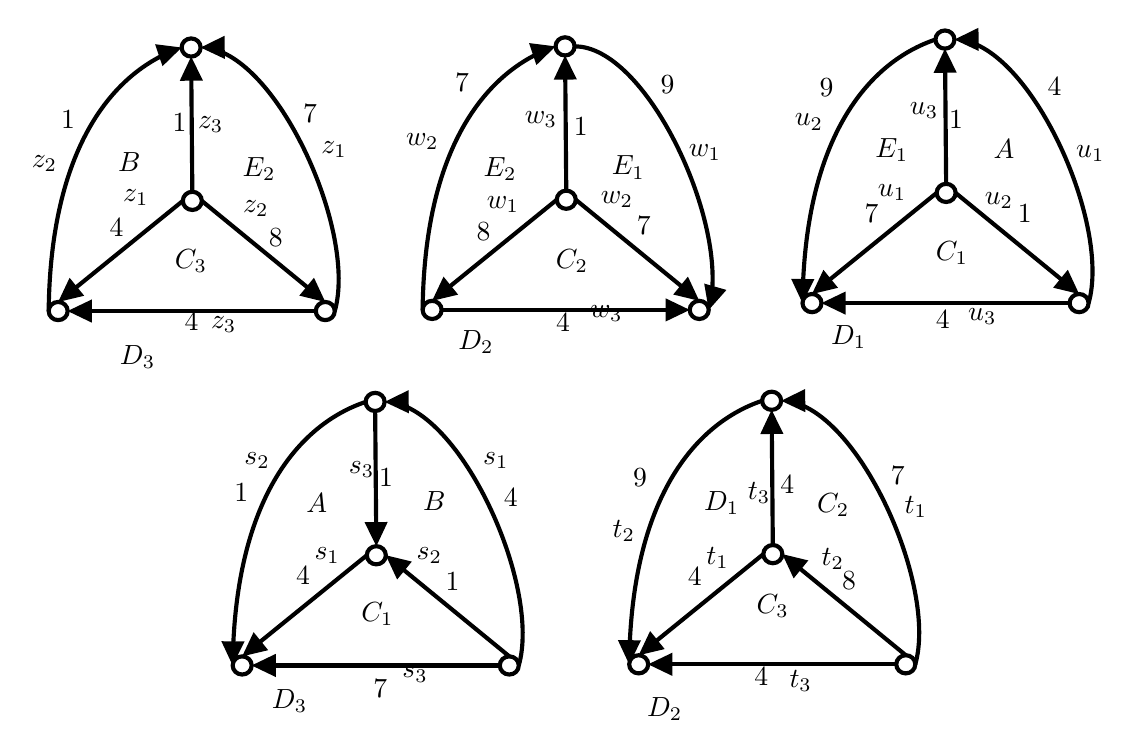
\begin{tikzpicture}[x=0.75pt,y=0.75pt,yscale=-1,xscale=1]
%uncomment if require: \path (0,498); %set diagram left start at 0, and has height of 498

%Shape: Ellipse [id:dp722498185471097] 
\draw  [line width=1.5]  (140.33,28.88) .. controls (140.33,26.46) and (142.38,24.5) .. (144.91,24.5) .. controls (147.43,24.5) and (149.48,26.46) .. (149.48,28.88) .. controls (149.48,31.29) and (147.43,33.25) .. (144.91,33.25) .. controls (142.38,33.25) and (140.33,31.29) .. (140.33,28.88) -- cycle ;
%Shape: Ellipse [id:dp09419658359942129] 
\draw  [line width=1.5]  (140.9,102.76) .. controls (140.9,100.34) and (142.95,98.38) .. (145.48,98.38) .. controls (148.01,98.38) and (150.05,100.34) .. (150.05,102.76) .. controls (150.05,105.18) and (148.01,107.14) .. (145.48,107.14) .. controls (142.95,107.14) and (140.9,105.18) .. (140.9,102.76) -- cycle ;
%Shape: Ellipse [id:dp4574028971026852] 
\draw  [line width=1.5]  (76.27,155.84) .. controls (76.27,153.42) and (78.32,151.46) .. (80.85,151.46) .. controls (83.37,151.46) and (85.42,153.42) .. (85.42,155.84) .. controls (85.42,158.26) and (83.37,160.22) .. (80.85,160.22) .. controls (78.32,160.22) and (76.27,158.26) .. (76.27,155.84) -- cycle ;
%Shape: Ellipse [id:dp012434768366862081] 
\draw  [line width=1.5]  (204.96,155.84) .. controls (204.96,153.42) and (207.01,151.46) .. (209.54,151.46) .. controls (212.06,151.46) and (214.11,153.42) .. (214.11,155.84) .. controls (214.11,158.26) and (212.06,160.22) .. (209.54,160.22) .. controls (207.01,160.22) and (204.96,158.26) .. (204.96,155.84) -- cycle ;
%Straight Lines [id:da7104639893284079] 
\draw [line width=1.5]    (144.94,37.25) -- (145.48,98.38) ;
\draw [shift={(144.91,33.25)}, rotate = 89.5] [fill={rgb, 255:red, 0; green, 0; blue, 0 }  ][line width=0.08]  [draw opacity=0] (11.61,-5.58) -- (0,0) -- (11.61,5.58) -- cycle    ;
%Straight Lines [id:da06252865798857044] 
\draw [line width=1.5]    (89.42,155.84) -- (204.96,155.84) ;
\draw [shift={(85.42,155.84)}, rotate = 0] [fill={rgb, 255:red, 0; green, 0; blue, 0 }  ][line width=0.08]  [draw opacity=0] (11.61,-5.58) -- (0,0) -- (11.61,5.58) -- cycle    ;
%Straight Lines [id:da8407976043494823] 
\draw [line width=1.5]    (83.95,148.94) -- (140.9,102.76) ;
\draw [shift={(80.85,151.46)}, rotate = 320.96] [fill={rgb, 255:red, 0; green, 0; blue, 0 }  ][line width=0.08]  [draw opacity=0] (11.61,-5.58) -- (0,0) -- (11.61,5.58) -- cycle    ;
%Straight Lines [id:da93252160050729] 
\draw [line width=1.5]    (150.05,102.76) -- (206.44,148.93) ;
\draw [shift={(209.54,151.46)}, rotate = 219.31] [fill={rgb, 255:red, 0; green, 0; blue, 0 }  ][line width=0.08]  [draw opacity=0] (11.61,-5.58) -- (0,0) -- (11.61,5.58) -- cycle    ;
%Curve Lines [id:da914075530376739] 
\draw [line width=1.5]    (76.27,155.84) .. controls (77.1,77.95) and (106.42,42.09) .. (137,30.09) ;
\draw [shift={(140.33,28.88)}, rotate = 161.42] [fill={rgb, 255:red, 0; green, 0; blue, 0 }  ][line width=0.08]  [draw opacity=0] (11.61,-5.58) -- (0,0) -- (11.61,5.58) -- cycle    ;
%Curve Lines [id:da5685611468391036] 
\draw [line width=1.5]    (153.73,29.26) .. controls (187.82,35.57) and (224.82,118.28) .. (214.11,155.84) ;
\draw [shift={(149.48,28.88)}, rotate = 359.55] [fill={rgb, 255:red, 0; green, 0; blue, 0 }  ][line width=0.08]  [draw opacity=0] (11.61,-5.58) -- (0,0) -- (11.61,5.58) -- cycle    ;
%Shape: Ellipse [id:dp9871169656532187] 
\draw  [line width=1.5]  (320.49,28.33) .. controls (320.49,25.91) and (322.54,23.95) .. (325.07,23.95) .. controls (327.6,23.95) and (329.65,25.91) .. (329.65,28.33) .. controls (329.65,30.75) and (327.6,32.71) .. (325.07,32.71) .. controls (322.54,32.71) and (320.49,30.75) .. (320.49,28.33) -- cycle ;
%Shape: Ellipse [id:dp4998971196831187] 
\draw  [line width=1.5]  (321.07,102.21) .. controls (321.07,99.79) and (323.12,97.83) .. (325.64,97.83) .. controls (328.17,97.83) and (330.22,99.79) .. (330.22,102.21) .. controls (330.22,104.63) and (328.17,106.59) .. (325.64,106.59) .. controls (323.12,106.59) and (321.07,104.63) .. (321.07,102.21) -- cycle ;
%Shape: Ellipse [id:dp5334863650227393] 
\draw  [line width=1.5]  (256.44,155.3) .. controls (256.44,152.88) and (258.49,150.92) .. (261.01,150.92) .. controls (263.54,150.92) and (265.59,152.88) .. (265.59,155.3) .. controls (265.59,157.71) and (263.54,159.67) .. (261.01,159.67) .. controls (258.49,159.67) and (256.44,157.71) .. (256.44,155.3) -- cycle ;
%Shape: Ellipse [id:dp8295563632609373] 
\draw  [line width=1.5]  (385.13,155.3) .. controls (385.13,152.88) and (387.17,150.92) .. (389.7,150.92) .. controls (392.23,150.92) and (394.28,152.88) .. (394.28,155.3) .. controls (394.28,157.71) and (392.23,159.67) .. (389.7,159.67) .. controls (387.17,159.67) and (385.13,157.71) .. (385.13,155.3) -- cycle ;
%Straight Lines [id:da6853527229248998] 
\draw [line width=1.5]    (325.11,36.71) -- (325.64,97.83) ;
\draw [shift={(325.07,32.71)}, rotate = 89.5] [fill={rgb, 255:red, 0; green, 0; blue, 0 }  ][line width=0.08]  [draw opacity=0] (11.61,-5.58) -- (0,0) -- (11.61,5.58) -- cycle    ;
%Straight Lines [id:da37663298733859474] 
\draw [line width=1.5]    (265.59,155.3) -- (381.13,155.3) ;
\draw [shift={(385.13,155.3)}, rotate = 180] [fill={rgb, 255:red, 0; green, 0; blue, 0 }  ][line width=0.08]  [draw opacity=0] (11.61,-5.58) -- (0,0) -- (11.61,5.58) -- cycle    ;
%Straight Lines [id:da1331834266330163] 
\draw [line width=1.5]    (264.12,148.4) -- (321.07,102.21) ;
\draw [shift={(261.01,150.92)}, rotate = 320.96] [fill={rgb, 255:red, 0; green, 0; blue, 0 }  ][line width=0.08]  [draw opacity=0] (11.61,-5.58) -- (0,0) -- (11.61,5.58) -- cycle    ;
%Straight Lines [id:da93580380730357] 
\draw [line width=1.5]    (330.22,102.21) -- (386.61,148.38) ;
\draw [shift={(389.7,150.92)}, rotate = 219.31] [fill={rgb, 255:red, 0; green, 0; blue, 0 }  ][line width=0.08]  [draw opacity=0] (11.61,-5.58) -- (0,0) -- (11.61,5.58) -- cycle    ;
%Curve Lines [id:da9473646706061418] 
\draw [line width=1.5]    (256.44,155.3) .. controls (257.26,77.4) and (286.59,41.55) .. (317.16,29.54) ;
\draw [shift={(320.49,28.33)}, rotate = 161.42] [fill={rgb, 255:red, 0; green, 0; blue, 0 }  ][line width=0.08]  [draw opacity=0] (11.61,-5.58) -- (0,0) -- (11.61,5.58) -- cycle    ;
%Curve Lines [id:da4025171529168252] 
\draw [line width=1.5]    (329.65,28.33) .. controls (363.77,28.06) and (403,110.96) .. (395.14,151.65) ;
\draw [shift={(394.28,155.3)}, rotate = 285.91] [fill={rgb, 255:red, 0; green, 0; blue, 0 }  ][line width=0.08]  [draw opacity=0] (11.61,-5.58) -- (0,0) -- (11.61,5.58) -- cycle    ;
%Shape: Ellipse [id:dp4598430040551579] 
\draw  [line width=1.5]  (503.52,25.04) .. controls (503.52,22.63) and (505.57,20.67) .. (508.09,20.67) .. controls (510.62,20.67) and (512.67,22.63) .. (512.67,25.04) .. controls (512.67,27.46) and (510.62,29.42) .. (508.09,29.42) .. controls (505.57,29.42) and (503.52,27.46) .. (503.52,25.04) -- cycle ;
%Shape: Ellipse [id:dp5035867782009985] 
\draw  [line width=1.5]  (504.09,98.93) .. controls (504.09,96.51) and (506.14,94.55) .. (508.67,94.55) .. controls (511.19,94.55) and (513.24,96.51) .. (513.24,98.93) .. controls (513.24,101.34) and (511.19,103.3) .. (508.67,103.3) .. controls (506.14,103.3) and (504.09,101.34) .. (504.09,98.93) -- cycle ;
%Shape: Ellipse [id:dp6235578561815645] 
\draw  [line width=1.5]  (439.46,152.01) .. controls (439.46,149.59) and (441.51,147.63) .. (444.04,147.63) .. controls (446.56,147.63) and (448.61,149.59) .. (448.61,152.01) .. controls (448.61,154.43) and (446.56,156.39) .. (444.04,156.39) .. controls (441.51,156.39) and (439.46,154.43) .. (439.46,152.01) -- cycle ;
%Shape: Ellipse [id:dp47621421692962784] 
\draw  [line width=1.5]  (568.15,152.01) .. controls (568.15,149.59) and (570.2,147.63) .. (572.73,147.63) .. controls (575.25,147.63) and (577.3,149.59) .. (577.3,152.01) .. controls (577.3,154.43) and (575.25,156.39) .. (572.73,156.39) .. controls (570.2,156.39) and (568.15,154.43) .. (568.15,152.01) -- cycle ;
%Straight Lines [id:da24752576794389303] 
\draw [line width=1.5]    (508.13,33.42) -- (508.67,94.55) ;
\draw [shift={(508.09,29.42)}, rotate = 89.5] [fill={rgb, 255:red, 0; green, 0; blue, 0 }  ][line width=0.08]  [draw opacity=0] (11.61,-5.58) -- (0,0) -- (11.61,5.58) -- cycle    ;
%Straight Lines [id:da2745160206955022] 
\draw [line width=1.5]    (452.61,152.01) -- (568.15,152.01) ;
\draw [shift={(448.61,152.01)}, rotate = 0] [fill={rgb, 255:red, 0; green, 0; blue, 0 }  ][line width=0.08]  [draw opacity=0] (11.61,-5.58) -- (0,0) -- (11.61,5.58) -- cycle    ;
%Straight Lines [id:da1251063457941054] 
\draw [line width=1.5]    (447.14,145.11) -- (504.09,98.93) ;
\draw [shift={(444.04,147.63)}, rotate = 320.96] [fill={rgb, 255:red, 0; green, 0; blue, 0 }  ][line width=0.08]  [draw opacity=0] (11.61,-5.58) -- (0,0) -- (11.61,5.58) -- cycle    ;
%Straight Lines [id:da8560302252250104] 
\draw [line width=1.5]    (513.24,98.93) -- (569.63,145.1) ;
\draw [shift={(572.73,147.63)}, rotate = 219.31] [fill={rgb, 255:red, 0; green, 0; blue, 0 }  ][line width=0.08]  [draw opacity=0] (11.61,-5.58) -- (0,0) -- (11.61,5.58) -- cycle    ;
%Curve Lines [id:da5942103699772806] 
\draw [line width=1.5]    (439.55,147.22) .. controls (441.58,69.88) and (472.41,35.5) .. (503.52,25.04) ;
\draw [shift={(439.46,152.01)}, rotate = 270.61] [fill={rgb, 255:red, 0; green, 0; blue, 0 }  ][line width=0.08]  [draw opacity=0] (11.61,-5.58) -- (0,0) -- (11.61,5.58) -- cycle    ;
%Curve Lines [id:da7202124541602778] 
\draw [line width=1.5]    (516.91,25.43) .. controls (551.01,31.74) and (588.01,114.45) .. (577.3,152.01) ;
\draw [shift={(512.67,25.04)}, rotate = 359.55] [fill={rgb, 255:red, 0; green, 0; blue, 0 }  ][line width=0.08]  [draw opacity=0] (11.61,-5.58) -- (0,0) -- (11.61,5.58) -- cycle    ;
%Shape: Ellipse [id:dp7971440912052996] 
\draw  [line width=1.5]  (228.98,199.62) .. controls (228.98,197.21) and (231.03,195.25) .. (233.56,195.25) .. controls (236.09,195.25) and (238.13,197.21) .. (238.13,199.62) .. controls (238.13,202.04) and (236.09,204) .. (233.56,204) .. controls (231.03,204) and (228.98,202.04) .. (228.98,199.62) -- cycle ;
%Shape: Ellipse [id:dp4840470955224502] 
\draw  [line width=1.5]  (229.55,273.51) .. controls (229.55,271.09) and (231.6,269.13) .. (234.13,269.13) .. controls (236.66,269.13) and (238.71,271.09) .. (238.71,273.51) .. controls (238.71,275.92) and (236.66,277.88) .. (234.13,277.88) .. controls (231.6,277.88) and (229.55,275.92) .. (229.55,273.51) -- cycle ;
%Shape: Ellipse [id:dp7205406460641789] 
\draw  [line width=1.5]  (164.92,326.59) .. controls (164.92,324.17) and (166.97,322.21) .. (169.5,322.21) .. controls (172.03,322.21) and (174.08,324.17) .. (174.08,326.59) .. controls (174.08,329.01) and (172.03,330.97) .. (169.5,330.97) .. controls (166.97,330.97) and (164.92,329.01) .. (164.92,326.59) -- cycle ;
%Shape: Ellipse [id:dp16212402515113167] 
\draw  [line width=1.5]  (293.61,326.59) .. controls (293.61,324.17) and (295.66,322.21) .. (298.19,322.21) .. controls (300.72,322.21) and (302.76,324.17) .. (302.76,326.59) .. controls (302.76,329.01) and (300.72,330.97) .. (298.19,330.97) .. controls (295.66,330.97) and (293.61,329.01) .. (293.61,326.59) -- cycle ;
%Straight Lines [id:da38679418807864374] 
\draw [line width=1.5]    (233.56,204) -- (234.1,265.13) ;
\draw [shift={(234.13,269.13)}, rotate = 269.5] [fill={rgb, 255:red, 0; green, 0; blue, 0 }  ][line width=0.08]  [draw opacity=0] (11.61,-5.58) -- (0,0) -- (11.61,5.58) -- cycle    ;
%Straight Lines [id:da7340741733057103] 
\draw [line width=1.5]    (178.08,326.59) -- (293.61,326.59) ;
\draw [shift={(174.08,326.59)}, rotate = 0] [fill={rgb, 255:red, 0; green, 0; blue, 0 }  ][line width=0.08]  [draw opacity=0] (11.61,-5.58) -- (0,0) -- (11.61,5.58) -- cycle    ;
%Straight Lines [id:da6492127454486433] 
\draw [line width=1.5]    (172.61,319.69) -- (229.55,273.51) ;
\draw [shift={(169.5,322.21)}, rotate = 320.96] [fill={rgb, 255:red, 0; green, 0; blue, 0 }  ][line width=0.08]  [draw opacity=0] (11.61,-5.58) -- (0,0) -- (11.61,5.58) -- cycle    ;
%Straight Lines [id:da1534318649264561] 
\draw [line width=1.5]    (241.8,276.04) -- (298.19,322.21) ;
\draw [shift={(238.71,273.51)}, rotate = 39.31] [fill={rgb, 255:red, 0; green, 0; blue, 0 }  ][line width=0.08]  [draw opacity=0] (11.61,-5.58) -- (0,0) -- (11.61,5.58) -- cycle    ;
%Curve Lines [id:da15708072815584284] 
\draw [line width=1.5]    (165.01,321.8) .. controls (167.04,244.46) and (197.87,210.08) .. (228.98,199.62) ;
\draw [shift={(164.92,326.59)}, rotate = 270.61] [fill={rgb, 255:red, 0; green, 0; blue, 0 }  ][line width=0.08]  [draw opacity=0] (11.61,-5.58) -- (0,0) -- (11.61,5.58) -- cycle    ;
%Curve Lines [id:da4532354822589155] 
\draw [line width=1.5]    (242.38,200.01) .. controls (276.47,206.32) and (313.47,289.03) .. (302.76,326.59) ;
\draw [shift={(238.13,199.62)}, rotate = 359.55] [fill={rgb, 255:red, 0; green, 0; blue, 0 }  ][line width=0.08]  [draw opacity=0] (11.61,-5.58) -- (0,0) -- (11.61,5.58) -- cycle    ;
%Shape: Ellipse [id:dp707487152357257] 
\draw  [line width=1.5]  (420.01,199.08) .. controls (420.01,196.66) and (422.06,194.7) .. (424.59,194.7) .. controls (427.12,194.7) and (429.17,196.66) .. (429.17,199.08) .. controls (429.17,201.5) and (427.12,203.46) .. (424.59,203.46) .. controls (422.06,203.46) and (420.01,201.5) .. (420.01,199.08) -- cycle ;
%Shape: Ellipse [id:dp2675712667635096] 
\draw  [line width=1.5]  (420.59,272.96) .. controls (420.59,270.54) and (422.63,268.58) .. (425.16,268.58) .. controls (427.69,268.58) and (429.74,270.54) .. (429.74,272.96) .. controls (429.74,275.38) and (427.69,277.34) .. (425.16,277.34) .. controls (422.63,277.34) and (420.59,275.38) .. (420.59,272.96) -- cycle ;
%Shape: Ellipse [id:dp04604583726861322] 
\draw  [line width=1.5]  (355.96,326.04) .. controls (355.96,323.63) and (358,321.67) .. (360.53,321.67) .. controls (363.06,321.67) and (365.11,323.63) .. (365.11,326.04) .. controls (365.11,328.46) and (363.06,330.42) .. (360.53,330.42) .. controls (358,330.42) and (355.96,328.46) .. (355.96,326.04) -- cycle ;
%Shape: Ellipse [id:dp527192499801234] 
\draw  [line width=1.5]  (484.64,326.04) .. controls (484.64,323.63) and (486.69,321.67) .. (489.22,321.67) .. controls (491.75,321.67) and (493.8,323.63) .. (493.8,326.04) .. controls (493.8,328.46) and (491.75,330.42) .. (489.22,330.42) .. controls (486.69,330.42) and (484.64,328.46) .. (484.64,326.04) -- cycle ;
%Straight Lines [id:da2748072495693461] 
\draw [line width=1.5]    (424.63,207.46) -- (425.16,268.58) ;
\draw [shift={(424.59,203.46)}, rotate = 89.5] [fill={rgb, 255:red, 0; green, 0; blue, 0 }  ][line width=0.08]  [draw opacity=0] (11.61,-5.58) -- (0,0) -- (11.61,5.58) -- cycle    ;
%Straight Lines [id:da8571687174187388] 
\draw [line width=1.5]    (369.11,326.04) -- (484.64,326.04) ;
\draw [shift={(365.11,326.04)}, rotate = 0] [fill={rgb, 255:red, 0; green, 0; blue, 0 }  ][line width=0.08]  [draw opacity=0] (11.61,-5.58) -- (0,0) -- (11.61,5.58) -- cycle    ;
%Straight Lines [id:da009179926411796768] 
\draw [line width=1.5]    (363.64,319.15) -- (420.59,272.96) ;
\draw [shift={(360.53,321.67)}, rotate = 320.96] [fill={rgb, 255:red, 0; green, 0; blue, 0 }  ][line width=0.08]  [draw opacity=0] (11.61,-5.58) -- (0,0) -- (11.61,5.58) -- cycle    ;
%Straight Lines [id:da09268248986267924] 
\draw [line width=1.5]    (432.83,275.49) -- (489.22,321.67) ;
\draw [shift={(429.74,272.96)}, rotate = 39.31] [fill={rgb, 255:red, 0; green, 0; blue, 0 }  ][line width=0.08]  [draw opacity=0] (11.61,-5.58) -- (0,0) -- (11.61,5.58) -- cycle    ;
%Curve Lines [id:da7275208733646754] 
\draw [line width=1.5]    (356.04,321.25) .. controls (358.07,243.91) and (388.91,209.54) .. (420.01,199.08) ;
\draw [shift={(355.96,326.04)}, rotate = 270.61] [fill={rgb, 255:red, 0; green, 0; blue, 0 }  ][line width=0.08]  [draw opacity=0] (11.61,-5.58) -- (0,0) -- (11.61,5.58) -- cycle    ;
%Curve Lines [id:da8929863303964553] 
\draw [line width=1.5]    (433.41,199.46) .. controls (467.51,205.77) and (504.5,288.48) .. (493.8,326.04) ;
\draw [shift={(429.17,199.08)}, rotate = 359.55] [fill={rgb, 255:red, 0; green, 0; blue, 0 }  ][line width=0.08]  [draw opacity=0] (11.61,-5.58) -- (0,0) -- (11.61,5.58) -- cycle    ;

% Text Node
\draw (135.57,124.53) node [anchor=north west][inner sep=0.75pt]    {$C_{3}$};
% Text Node
\draw (108.19,78.19) node [anchor=north west][inner sep=0.75pt]    {$B$};
% Text Node
\draw (168.24,80.2) node [anchor=north west][inner sep=0.75pt]    {$E_{2}$};
% Text Node
\draw (109.12,171.05) node [anchor=north west][inner sep=0.75pt]    {$D_{3}$};
% Text Node
\draw (104.18,109.93) node [anchor=north west][inner sep=0.75pt]    {$4$};
% Text Node
\draw (180.82,114.59) node [anchor=north west][inner sep=0.75pt]    {$8$};
% Text Node
\draw (140.22,155.36) node [anchor=north west][inner sep=0.75pt]    {$4$};
% Text Node
\draw (134.5,59.31) node [anchor=north west][inner sep=0.75pt]    {$1$};
% Text Node
\draw (80.73,57.67) node [anchor=north west][inner sep=0.75pt]    {$1$};
% Text Node
\draw (197.41,54.93) node [anchor=north west][inner sep=0.75pt]    {$7$};
% Text Node
\draw (284.35,80.2) node [anchor=north west][inner sep=0.75pt]    {$E_{2}$};
% Text Node
\draw (346.12,79.65) node [anchor=north west][inner sep=0.75pt]    {$E_{1}$};
% Text Node
\draw (319.17,124.53) node [anchor=north west][inner sep=0.75pt]    {$C_{2}$};
% Text Node
\draw (272.13,163.66) node [anchor=north west][inner sep=0.75pt]    {$D_{2}$};
% Text Node
\draw (280.92,111.85) node [anchor=north west][inner sep=0.75pt]    {$8$};
% Text Node
\draw (358.13,109.11) node [anchor=north west][inner sep=0.75pt]    {$7$};
% Text Node
\draw (319.24,155.63) node [anchor=north west][inner sep=0.75pt]    {$4$};
% Text Node
\draw (327.82,60.95) node [anchor=north west][inner sep=0.75pt]    {$1$};
% Text Node
\draw (270.62,40.16) node [anchor=north west][inner sep=0.75pt]    {$7$};
% Text Node
\draw (369.57,40.7) node [anchor=north west][inner sep=0.75pt]    {$9$};
% Text Node
\draw (473.09,71.17) node [anchor=north west][inner sep=0.75pt]    {$E_{1}$};
% Text Node
\draw (530.07,71.9) node [anchor=north west][inner sep=0.75pt]    {$A$};
% Text Node
\draw (502.19,120.97) node [anchor=north west][inner sep=0.75pt]    {$C_{1}$};
% Text Node
\draw (451.72,161.47) node [anchor=north west][inner sep=0.75pt]    {$D_{1}$};
% Text Node
\draw (467.94,103.09) node [anchor=north west][inner sep=0.75pt]    {$7$};
% Text Node
\draw (508.55,57.67) node [anchor=north west][inner sep=0.75pt]    {$1$};
% Text Node
\draw (541.72,103.09) node [anchor=north west][inner sep=0.75pt]    {$1$};
% Text Node
\draw (502.26,153.99) node [anchor=north west][inner sep=0.75pt]    {$4$};
% Text Node
\draw (556.02,41.8) node [anchor=north west][inner sep=0.75pt]    {$4$};
% Text Node
\draw (446.21,42.35) node [anchor=north west][inner sep=0.75pt]    {$9$};
% Text Node
\draw (198.91,242.37) node [anchor=north west][inner sep=0.75pt]    {$A$};
% Text Node
\draw (255.18,241.28) node [anchor=north west][inner sep=0.75pt]    {$B$};
% Text Node
\draw (225.37,294.73) node [anchor=north west][inner sep=0.75pt]    {$C_{1}$};
% Text Node
\draw (182.33,336.87) node [anchor=north west][inner sep=0.75pt]    {$D_{3}$};
% Text Node
\draw (390.52,241.1) node [anchor=north west][inner sep=0.75pt]    {$D_{1}$};
% Text Node
\draw (445,242.19) node [anchor=north west][inner sep=0.75pt]    {$C_{2}$};
% Text Node
\draw (415.83,290.9) node [anchor=north west][inner sep=0.75pt]    {$C_{3}$};
% Text Node
\draw (363.07,340.7) node [anchor=north west][inner sep=0.75pt]    {$D_{2}$};
% Text Node
\draw (164.24,237.72) node [anchor=north west][inner sep=0.75pt]    {$1$};
% Text Node
\draw (234.02,230.06) node [anchor=north west][inner sep=0.75pt]    {$1$};
% Text Node
\draw (266.04,280.41) node [anchor=north west][inner sep=0.75pt]    {$1$};
% Text Node
\draw (193.98,277.67) node [anchor=north west][inner sep=0.75pt]    {$4$};
% Text Node
\draw (294.07,239.91) node [anchor=north west][inner sep=0.75pt]    {$4$};
% Text Node
\draw (231.16,331.85) node [anchor=north west][inner sep=0.75pt]    {$7$};
% Text Node
\draw (382.72,278.22) node [anchor=north west][inner sep=0.75pt]    {$4$};
% Text Node
\draw (427.33,233.89) node [anchor=north west][inner sep=0.75pt]    {$4$};
% Text Node
\draw (414.75,326.38) node [anchor=north west][inner sep=0.75pt]    {$4$};
% Text Node
\draw (356.41,230.06) node [anchor=north west][inner sep=0.75pt]    {$9$};
% Text Node
\draw (457.08,279.86) node [anchor=north west][inner sep=0.75pt]    {$8$};
% Text Node
\draw (480.53,229.51) node [anchor=north west][inner sep=0.75pt]    {$7$};
% Text Node
\draw (110.69,95.8) node [anchor=north west][inner sep=0.75pt]    {$z_{1}$};
% Text Node
\draw (206.21,72.81) node [anchor=north west][inner sep=0.75pt]    {$z_{1}$};
% Text Node
\draw (168.46,101.27) node [anchor=north west][inner sep=0.75pt]    {$z_{2}$};
% Text Node
\draw (66.65,79.38) node [anchor=north west][inner sep=0.75pt]    {$z_{2}$};
% Text Node
\draw (153.01,157.09) node [anchor=north west][inner sep=0.75pt]    {$z_{3}$};
% Text Node
\draw (146.72,60.77) node [anchor=north west][inner sep=0.75pt]    {$z_{3}$};
% Text Node
\draw (285.92,99.08) node [anchor=north west][inner sep=0.75pt]    {$w_{1}$};
% Text Node
\draw (383.16,73.91) node [anchor=north west][inner sep=0.75pt]    {$w_{1}$};
% Text Node
\draw (340.83,96.89) node [anchor=north west][inner sep=0.75pt]    {$w_{2}$};
% Text Node
\draw (247.03,68.98) node [anchor=north west][inner sep=0.75pt]    {$w_{2}$};
% Text Node
\draw (335.68,151.62) node [anchor=north west][inner sep=0.75pt]    {$w_{3}$};
% Text Node
\draw (304.23,58.04) node [anchor=north west][inner sep=0.75pt]    {$w_{3}$};
% Text Node
\draw (474.31,93.34) node [anchor=north west][inner sep=0.75pt]    {$u_{1}$};
% Text Node
\draw (569.83,74.73) node [anchor=north west][inner sep=0.75pt]    {$u_{1}$};
% Text Node
\draw (525.78,97.17) node [anchor=north west][inner sep=0.75pt]    {$u_{2}$};
% Text Node
\draw (434.27,59.41) node [anchor=north west][inner sep=0.75pt]    {$u_{2}$};
% Text Node
\draw (517.78,152.99) node [anchor=north west][inner sep=0.75pt]    {$u_{3}$};
% Text Node
\draw (489.75,53.93) node [anchor=north west][inner sep=0.75pt]    {$u_{3}$};
% Text Node
\draw (202.85,268.46) node [anchor=north west][inner sep=0.75pt]    {$s_{1}$};
% Text Node
\draw (284.06,222.49) node [anchor=north west][inner sep=0.75pt]    {$s_{1}$};
% Text Node
\draw (252.03,268.46) node [anchor=north west][inner sep=0.75pt]    {$s_{2}$};
% Text Node
\draw (169.1,222.49) node [anchor=north west][inner sep=0.75pt]    {$s_{2}$};
% Text Node
\draw (219.43,226.87) node [anchor=north west][inner sep=0.75pt]    {$s_{3}$};
% Text Node
\draw (245.17,325.38) node [anchor=north west][inner sep=0.75pt]    {$s_{3}$};
% Text Node
\draw (391.66,268.19) node [anchor=north west][inner sep=0.75pt]    {$t_{1}$};
% Text Node
\draw (487.18,243.56) node [anchor=north west][inner sep=0.75pt]    {$t_{1}$};
% Text Node
\draw (447.14,268.74) node [anchor=north west][inner sep=0.75pt]    {$t_{2}$};
% Text Node
\draw (346.48,255.06) node [anchor=north west][inner sep=0.75pt]    {$t_{2}$};
% Text Node
\draw (431.7,327.3) node [anchor=north west][inner sep=0.75pt]    {$t_{3}$};
% Text Node
\draw (411.68,237) node [anchor=north west][inner sep=0.75pt]    {$t_{3}$};


\end{tikzpicture}
    \caption{Triangulación topológica ideal del nudo $6_1$}
\end{figure}
Con esto ya podemos empezar a pensar primero en ecuaciones de pegado, Observe que dotamos a cada tetraedro de variables $z_i,w_i,u_i,s_i$ y $t_i$, con $i=1,2,3$, al igual que en el caso del nudo de ocho primero solo mantenemos el invariante de arista para aristas opuestas, la ecuaciones de pegado por arista son
\begin{itemize}
    \item \textbf{Arista 1:} $z_2z_3w_3u_2u_3s_2^2s_3=1.$
    \item \textbf{Arista 4:} $z_1z_3w_3u_1u_3s_1^2t_1t_3^2=1.$
    \item \textbf{Arista 7:} $z_1w_2^2u_1s_3t_1=1.$
    \item \textbf{Arista 8:} $z_2w_1t_2=1.$
    \item \textbf{Arista 9:} $w_1u_2t_2=1.$
\end{itemize}
Haciendo las sustituciones $z_1=z,w_1=w,u_1=u,s_1=s$ y $t_1=t$ y usando el lema 4.1 obtenemos el siguiente sistema de ecuaciones no lineal
$$\begin{cases}
    \dfrac{1-w}{zu(1-s)sw}=1\\
    \\
    \dfrac{(z-1)(w-1)(u-1)s^2(t-1)^2}{wt}=1\\
    \\
    \dfrac{zu(s-1)t}{(1-w)^2s}=1\\
    \\
    \dfrac{w}{(1-z)(1-t)}=1\\
    \\
    \dfrac{w}{(1-u)(1-t)}=1
\end{cases}$$
Algunas condiciones son fáciles de deducir, como por ejemplo que $z=u$, pero resolver este sistema e incluso otros sobrepasa la capacidad de calculo en general cuando se trata de determinar la parametrizacion de soluciones, por lo que  en general lo mejor es usar software para solucionar. Cuando se trata de las ecuaciones de completez pasa algo incluso mas complicado y es al momento de truncar los tetraedros en este caso se generan 20 triángulos que se necesitan pegar de manera adecuada siguiendo las identificaciones de las caras, mas esta tarea se salio de mis manos y entra en juego la ayuda de herramientas computacionales.

\subsection{Ecuaciones de pegado y completes para el enlace de Whitehead}

Al igual que antes ya teníamos dos poliedros ideales (pirámides) que reflejaban el complemento del enlace de Whitehead, en este caso la división en tetraedros es casi inmediata, pero seguiremos la idea del anterior ejemplo por consistencia. Primero dividimos en ambos poliedros la cara $G$ por medio de una arista extra
\begin{figure}[H]
\centering
%!TEX root = ./main.tex



\tikzset{every picture/.style={line width=0.75pt}} %set default line width to 0.75pt        

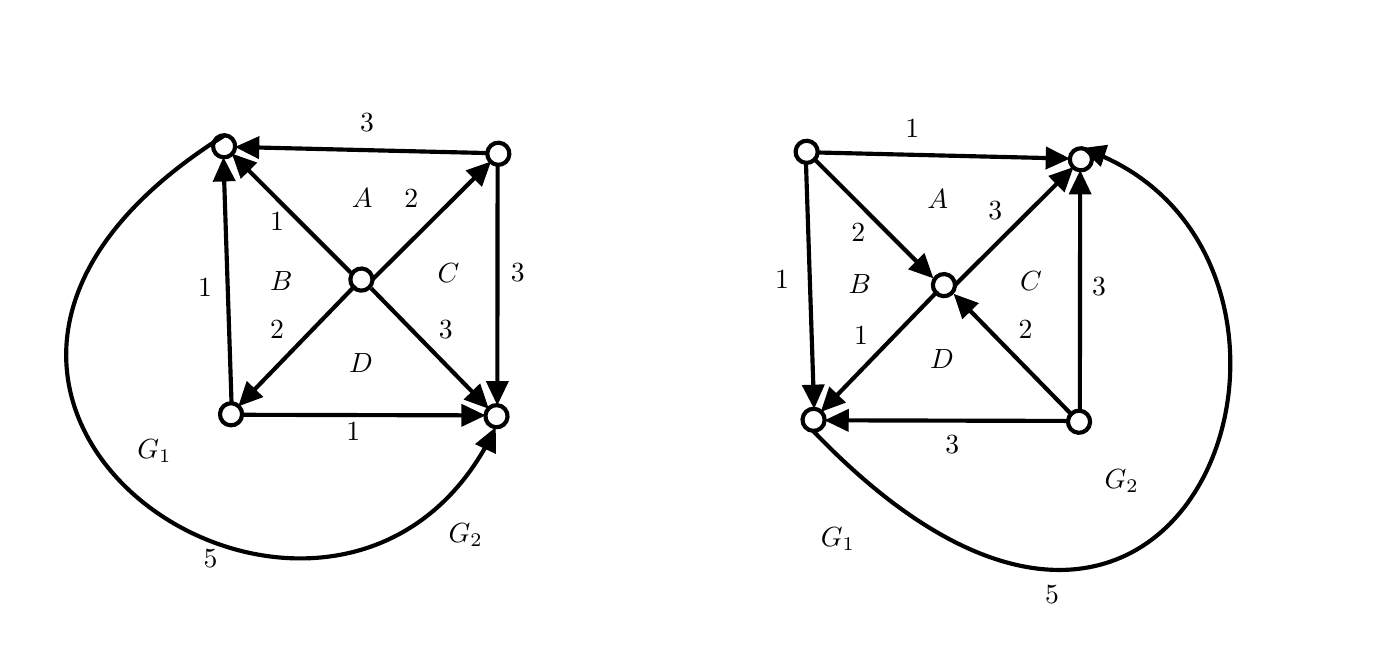
\begin{tikzpicture}[x=0.75pt,y=0.75pt,yscale=-1,xscale=1]
%uncomment if require: \path (0,498); %set diagram left start at 0, and has height of 498
\path[use as bounding box] (20,10) rectangle (660,300);
%Shape: Circle [id:dp8563981245220138] 
\draw  [line width=1.5]  (109.32,66.82) .. controls (109.5,63.88) and (112.03,61.64) .. (114.97,61.82) .. controls (117.91,62.01) and (120.15,64.54) .. (119.96,67.48) .. controls (119.78,70.42) and (117.25,72.65) .. (114.31,72.47) .. controls (111.37,72.29) and (109.14,69.76) .. (109.32,66.82) -- cycle ;
%Shape: Circle [id:dp3520905591144071] 
\draw  [line width=1.5]  (175.47,131.04) .. controls (175.65,128.1) and (178.18,125.86) .. (181.12,126.04) .. controls (184.06,126.23) and (186.3,128.76) .. (186.12,131.7) .. controls (185.93,134.64) and (183.4,136.87) .. (180.46,136.69) .. controls (177.52,136.51) and (175.29,133.98) .. (175.47,131.04) -- cycle ;
%Straight Lines [id:da29309615585626436] 
\draw [line width=1.5]    (121.25,73.55) -- (175.65,128.04) ;
\draw [shift={(118.43,70.72)}, rotate = 45.05] [fill={rgb, 255:red, 0; green, 0; blue, 0 }  ][line width=0.08]  [draw opacity=0] (11.61,-5.58) -- (0,0) -- (11.61,5.58) -- cycle    ;
%Shape: Circle [id:dp7112383425029831] 
\draw  [line width=1.5]  (247.1,65.43) .. controls (250.04,65.61) and (252.27,68.15) .. (252.08,71.09) .. controls (251.9,74.03) and (249.36,76.26) .. (246.42,76.07) .. controls (243.49,75.88) and (241.25,73.35) .. (241.44,70.41) .. controls (241.63,67.47) and (244.16,65.24) .. (247.1,65.43) -- cycle ;
%Straight Lines [id:da41995557597045774] 
\draw [line width=1.5]    (240.35,77.35) -- (185.78,131.68) ;
\draw [shift={(243.18,74.53)}, rotate = 135.13] [fill={rgb, 255:red, 0; green, 0; blue, 0 }  ][line width=0.08]  [draw opacity=0] (11.61,-5.58) -- (0,0) -- (11.61,5.58) -- cycle    ;
%Shape: Circle [id:dp5575025818197289] 
\draw  [line width=1.5]  (117.75,201.6) .. controls (114.81,201.47) and (112.53,198.97) .. (112.66,196.03) .. controls (112.79,193.09) and (115.28,190.81) .. (118.22,190.94) .. controls (121.17,191.07) and (123.45,193.57) .. (123.31,196.51) .. controls (123.18,199.45) and (120.69,201.73) .. (117.75,201.6) -- cycle ;
%Straight Lines [id:da4725169852169093] 
\draw [line width=1.5]    (124.28,189.55) -- (177.82,134.21) ;
\draw [shift={(121.49,192.42)}, rotate = 314.06] [fill={rgb, 255:red, 0; green, 0; blue, 0 }  ][line width=0.08]  [draw opacity=0] (11.61,-5.58) -- (0,0) -- (11.61,5.58) -- cycle    ;
%Shape: Circle [id:dp9549973004430545] 
\draw  [line width=1.5]  (251.2,197.58) .. controls (250.98,200.52) and (248.43,202.72) .. (245.49,202.51) .. controls (242.55,202.29) and (240.34,199.74) .. (240.56,196.8) .. controls (240.77,193.86) and (243.33,191.66) .. (246.27,191.87) .. controls (249.2,192.09) and (251.41,194.64) .. (251.2,197.58) -- cycle ;
%Straight Lines [id:da14548168825025642] 
\draw [line width=1.5]    (239.34,190.71) -- (185.54,135.63) ;
\draw [shift={(242.13,193.57)}, rotate = 225.68] [fill={rgb, 255:red, 0; green, 0; blue, 0 }  ][line width=0.08]  [draw opacity=0] (11.61,-5.58) -- (0,0) -- (11.61,5.58) -- cycle    ;
%Straight Lines [id:da04138952431338294] 
\draw [line width=1.5]    (123.31,196.51) -- (236.56,196.79) ;
\draw [shift={(240.56,196.8)}, rotate = 180.14] [fill={rgb, 255:red, 0; green, 0; blue, 0 }  ][line width=0.08]  [draw opacity=0] (11.61,-5.58) -- (0,0) -- (11.61,5.58) -- cycle    ;
%Straight Lines [id:da6360614459550309] 
\draw [line width=1.5]    (114.44,76.47) -- (118.22,190.94) ;
\draw [shift={(114.31,72.47)}, rotate = 88.11] [fill={rgb, 255:red, 0; green, 0; blue, 0 }  ][line width=0.08]  [draw opacity=0] (11.61,-5.58) -- (0,0) -- (11.61,5.58) -- cycle    ;
%Straight Lines [id:da22900843394258874] 
\draw [line width=1.5]    (123.96,67.57) -- (241.44,70.41) ;
\draw [shift={(119.96,67.48)}, rotate = 1.38] [fill={rgb, 255:red, 0; green, 0; blue, 0 }  ][line width=0.08]  [draw opacity=0] (11.61,-5.58) -- (0,0) -- (11.61,5.58) -- cycle    ;
%Straight Lines [id:da9297989788033489] 
\draw [line width=1.5]    (246.42,76.07) -- (246.27,187.87) ;
\draw [shift={(246.27,191.87)}, rotate = 270.08] [fill={rgb, 255:red, 0; green, 0; blue, 0 }  ][line width=0.08]  [draw opacity=0] (11.61,-5.58) -- (0,0) -- (11.61,5.58) -- cycle    ;
%Shape: Circle [id:dp6983363055718416] 
\draw  [line width=1.5]  (389.99,69.48) .. controls (390.17,66.54) and (392.7,64.31) .. (395.64,64.49) .. controls (398.58,64.67) and (400.81,67.2) .. (400.63,70.14) .. controls (400.45,73.08) and (397.92,75.32) .. (394.98,75.14) .. controls (392.04,74.96) and (389.8,72.42) .. (389.99,69.48) -- cycle ;
%Shape: Circle [id:dp34637775441133845] 
\draw  [line width=1.5]  (456.14,133.7) .. controls (456.32,130.76) and (458.85,128.53) .. (461.79,128.71) .. controls (464.73,128.89) and (466.96,131.42) .. (466.78,134.36) .. controls (466.6,137.3) and (464.07,139.54) .. (461.13,139.36) .. controls (458.19,139.17) and (455.95,136.64) .. (456.14,133.7) -- cycle ;
%Straight Lines [id:da32489783251721505] 
\draw [line width=1.5]    (399.09,73.39) -- (453.5,127.88) ;
\draw [shift={(456.32,130.71)}, rotate = 225.05] [fill={rgb, 255:red, 0; green, 0; blue, 0 }  ][line width=0.08]  [draw opacity=0] (11.61,-5.58) -- (0,0) -- (11.61,5.58) -- cycle    ;
%Shape: Circle [id:dp04140762256709696] 
\draw  [line width=1.5]  (527.77,68.09) .. controls (530.71,68.28) and (532.94,70.81) .. (532.75,73.75) .. controls (532.57,76.69) and (530.03,78.92) .. (527.09,78.74) .. controls (524.15,78.55) and (521.92,76.02) .. (522.11,73.08) .. controls (522.29,70.14) and (524.83,67.91) .. (527.77,68.09) -- cycle ;
%Straight Lines [id:da0022087921748601413] 
\draw [line width=1.5]    (521.01,80.02) -- (466.45,134.34) ;
\draw [shift={(523.85,77.2)}, rotate = 135.13] [fill={rgb, 255:red, 0; green, 0; blue, 0 }  ][line width=0.08]  [draw opacity=0] (11.61,-5.58) -- (0,0) -- (11.61,5.58) -- cycle    ;
%Shape: Circle [id:dp13672754996963388] 
\draw  [line width=1.5]  (398.41,204.26) .. controls (395.47,204.13) and (393.19,201.64) .. (393.32,198.7) .. controls (393.46,195.76) and (395.95,193.48) .. (398.89,193.61) .. controls (401.83,193.74) and (404.11,196.23) .. (403.98,199.17) .. controls (403.85,202.12) and (401.36,204.4) .. (398.41,204.26) -- cycle ;
%Straight Lines [id:da052100170009540814] 
\draw [line width=1.5]    (404.94,192.21) -- (458.48,136.88) ;
\draw [shift={(402.16,195.09)}, rotate = 314.06] [fill={rgb, 255:red, 0; green, 0; blue, 0 }  ][line width=0.08]  [draw opacity=0] (11.61,-5.58) -- (0,0) -- (11.61,5.58) -- cycle    ;
%Shape: Circle [id:dp8069072010758881] 
\draw  [line width=1.5]  (531.86,200.25) .. controls (531.65,203.18) and (529.09,205.39) .. (526.16,205.18) .. controls (523.22,204.96) and (521.01,202.41) .. (521.22,199.47) .. controls (521.44,196.53) and (523.99,194.32) .. (526.93,194.54) .. controls (529.87,194.75) and (532.08,197.31) .. (531.86,200.25) -- cycle ;
%Straight Lines [id:da801530605139214] 
\draw [line width=1.5]    (522.8,196.24) -- (469,141.16) ;
\draw [shift={(466.2,138.29)}, rotate = 45.68] [fill={rgb, 255:red, 0; green, 0; blue, 0 }  ][line width=0.08]  [draw opacity=0] (11.61,-5.58) -- (0,0) -- (11.61,5.58) -- cycle    ;
%Straight Lines [id:da7355128204598104] 
\draw [line width=1.5]    (407.98,199.18) -- (521.22,199.47) ;
\draw [shift={(403.98,199.17)}, rotate = 0.14] [fill={rgb, 255:red, 0; green, 0; blue, 0 }  ][line width=0.08]  [draw opacity=0] (11.61,-5.58) -- (0,0) -- (11.61,5.58) -- cycle    ;
%Straight Lines [id:da7937596572289117] 
\draw [line width=1.5]    (394.98,75.14) -- (398.76,189.61) ;
\draw [shift={(398.89,193.61)}, rotate = 268.11] [fill={rgb, 255:red, 0; green, 0; blue, 0 }  ][line width=0.08]  [draw opacity=0] (11.61,-5.58) -- (0,0) -- (11.61,5.58) -- cycle    ;
%Straight Lines [id:da2955657521942342] 
\draw [line width=1.5]    (400.63,70.14) -- (518.11,72.98) ;
\draw [shift={(522.11,73.08)}, rotate = 181.38] [fill={rgb, 255:red, 0; green, 0; blue, 0 }  ][line width=0.08]  [draw opacity=0] (11.61,-5.58) -- (0,0) -- (11.61,5.58) -- cycle    ;
%Straight Lines [id:da5139882653554566] 
\draw [line width=1.5]    (527.09,82.74) -- (526.93,194.54) ;
\draw [shift={(527.09,78.74)}, rotate = 90.08] [fill={rgb, 255:red, 0; green, 0; blue, 0 }  ][line width=0.08]  [draw opacity=0] (11.61,-5.58) -- (0,0) -- (11.61,5.58) -- cycle    ;
%Curve Lines [id:da6493881684844067] 
\draw [line width=1.5]    (114.97,61.82) .. controls (-87.98,189.03) and (169.07,357.97) .. (244.37,204.84) ;
\draw [shift={(245.49,202.51)}, rotate = 115.16] [fill={rgb, 255:red, 0; green, 0; blue, 0 }  ][line width=0.08]  [draw opacity=0] (11.61,-5.58) -- (0,0) -- (11.61,5.58) -- cycle    ;
%Curve Lines [id:da7408599747443351] 
\draw [line width=1.5]    (398.41,204.26) .. controls (582.74,396.7) and (670.78,118.47) .. (529.91,68.82) ;
\draw [shift={(527.77,68.09)}, rotate = 18.29] [fill={rgb, 255:red, 0; green, 0; blue, 0 }  ][line width=0.08]  [draw opacity=0] (11.61,-5.58) -- (0,0) -- (11.61,5.58) -- cycle    ;

% Text Node
\draw (174.67,86.07) node [anchor=north west][inner sep=0.75pt]    {$A$};
% Text Node
\draw (452,86.73) node [anchor=north west][inner sep=0.75pt]    {$A$};
% Text Node
\draw (135.33,126.07) node [anchor=north west][inner sep=0.75pt]    {$B$};
% Text Node
\draw (414,127.4) node [anchor=north west][inner sep=0.75pt]    {$B$};
% Text Node
\draw (216,122.07) node [anchor=north west][inner sep=0.75pt]    {$C$};
% Text Node
\draw (496.67,126.07) node [anchor=north west][inner sep=0.75pt]    {$C$};
% Text Node
\draw (173.33,165.4) node [anchor=north west][inner sep=0.75pt]    {$D$};
% Text Node
\draw (453.33,163.4) node [anchor=north west][inner sep=0.75pt]    {$D$};
% Text Node
\draw (100.67,129.4) node [anchor=north west][inner sep=0.75pt]    {$1$};
% Text Node
\draw (135.33,97.4) node [anchor=north west][inner sep=0.75pt]    {$1$};
% Text Node
\draw (172,198.73) node [anchor=north west][inner sep=0.75pt]    {$1$};
% Text Node
\draw (178.67,49.73) node [anchor=north west][inner sep=0.75pt]    {$3$};
% Text Node
\draw (251.33,122.4) node [anchor=north west][inner sep=0.75pt]    {$3$};
% Text Node
\draw (216.67,149.73) node [anchor=north west][inner sep=0.75pt]    {$3$};
% Text Node
\draw (135.33,149.73) node [anchor=north west][inner sep=0.75pt]    {$2$};
% Text Node
\draw (200,86.4) node [anchor=north west][inner sep=0.75pt]    {$2$};
% Text Node
\draw (378.67,125.4) node [anchor=north west][inner sep=0.75pt]    {$1$};
% Text Node
\draw (416.67,152.73) node [anchor=north west][inner sep=0.75pt]    {$1$};
% Text Node
\draw (441.33,52.73) node [anchor=north west][inner sep=0.75pt]    {$1$};
% Text Node
\draw (531.33,129.07) node [anchor=north west][inner sep=0.75pt]    {$3$};
% Text Node
\draw (481.33,92.4) node [anchor=north west][inner sep=0.75pt]    {$3$};
% Text Node
\draw (460.67,205.07) node [anchor=north west][inner sep=0.75pt]    {$3$};
% Text Node
\draw (415.33,103.07) node [anchor=north west][inner sep=0.75pt]    {$2$};
% Text Node
\draw (496,149.73) node [anchor=north west][inner sep=0.75pt]    {$2$};
% Text Node
\draw (71.33,206.73) node [anchor=north west][inner sep=0.75pt]    {$G_{1}$};
% Text Node
\draw (221.33,247.4) node [anchor=north west][inner sep=0.75pt]    {$G_{2}$};
% Text Node
\draw (103.33,260.07) node [anchor=north west][inner sep=0.75pt]    {$5$};
% Text Node
\draw (537.33,221.4) node [anchor=north west][inner sep=0.75pt]    {$G_{2}$};
% Text Node
\draw (400.67,249.4) node [anchor=north west][inner sep=0.75pt]    {$G_{1}$};
% Text Node
\draw (508.67,277.4) node [anchor=north west][inner sep=0.75pt]    {$5$};


\end{tikzpicture}
    \caption{División cara $G$ en los poliedros}
\end{figure}
Nuevamente es incluso mas facil que antes, basta con que en el poliedro de arriba se separen las caras $B,D,G_1$ del diagrama y se agregue una nueva cara $H_1$ y similarmente en el de abajo separar $C,D,G_2$ y agregar una nueva cara $H_2$ como se muestra a continuación
\begin{figure}[H]
\centering
%!TEX root = ./main.tex


\tikzset{every picture/.style={line width=0.75pt}} %set default line width to 0.75pt        

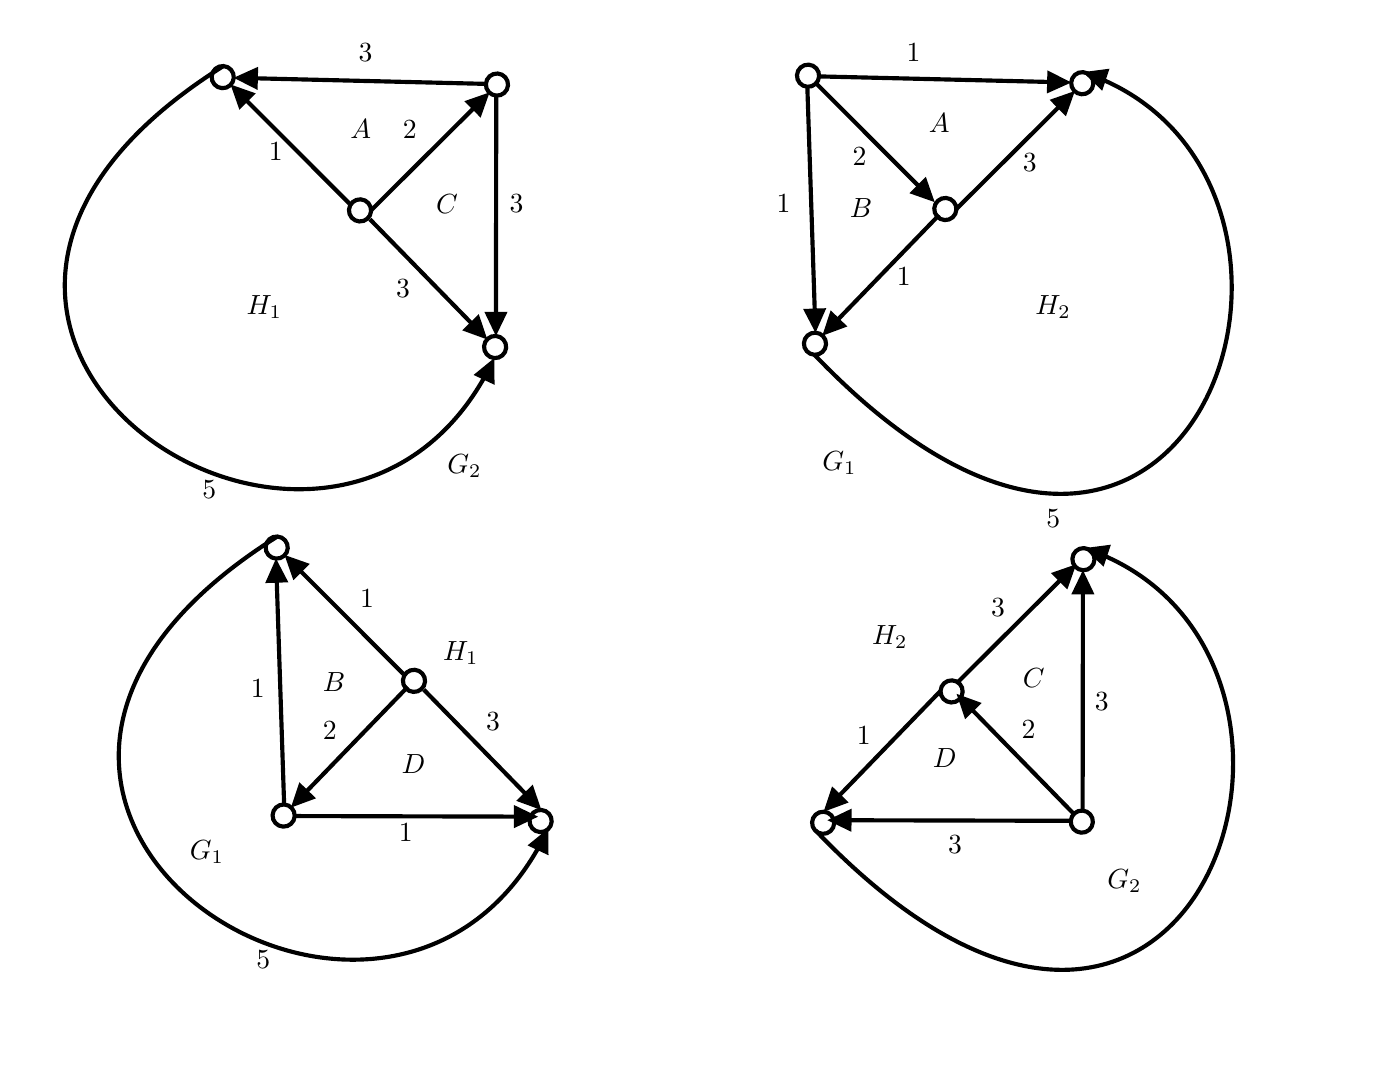
\begin{tikzpicture}[x=0.75pt,y=0.75pt,yscale=-1,xscale=1]
%uncomment if require: \path (0,498); %set diagram left start at 0, and has height of 498
\path[use as bounding box] (20,10) rectangle (660,500);
%Shape: Circle [id:dp8563981245220138] 
\draw  [line width=1.5]  (108.65,33.48) .. controls (108.83,30.54) and (111.37,28.31) .. (114.31,28.49) .. controls (117.24,28.67) and (119.48,31.2) .. (119.3,34.14) .. controls (119.12,37.08) and (116.58,39.32) .. (113.64,39.14) .. controls (110.7,38.96) and (108.47,36.42) .. (108.65,33.48) -- cycle ;
%Shape: Circle [id:dp3520905591144071] 
\draw  [line width=1.5]  (174.8,97.7) .. controls (174.98,94.76) and (177.52,92.53) .. (180.46,92.71) .. controls (183.4,92.89) and (185.63,95.42) .. (185.45,98.36) .. controls (185.27,101.3) and (182.74,103.54) .. (179.8,103.36) .. controls (176.86,103.17) and (174.62,100.64) .. (174.8,97.7) -- cycle ;
%Straight Lines [id:da29309615585626436] 
\draw [line width=1.5]    (120.59,40.22) -- (174.99,94.71) ;
\draw [shift={(117.76,37.39)}, rotate = 45.05] [fill={rgb, 255:red, 0; green, 0; blue, 0 }  ][line width=0.08]  [draw opacity=0] (11.61,-5.58) -- (0,0) -- (11.61,5.58) -- cycle    ;
%Shape: Circle [id:dp7112383425029831] 
\draw  [line width=1.5]  (246.43,32.09) .. controls (249.37,32.28) and (251.6,34.81) .. (251.42,37.75) .. controls (251.23,40.69) and (248.7,42.92) .. (245.76,42.74) .. controls (242.82,42.55) and (240.59,40.02) .. (240.77,37.08) .. controls (240.96,34.14) and (243.49,31.91) .. (246.43,32.09) -- cycle ;
%Straight Lines [id:da41995557597045774] 
\draw [line width=1.5]    (239.68,44.02) -- (185.12,98.34) ;
\draw [shift={(242.52,41.2)}, rotate = 135.13] [fill={rgb, 255:red, 0; green, 0; blue, 0 }  ][line width=0.08]  [draw opacity=0] (11.61,-5.58) -- (0,0) -- (11.61,5.58) -- cycle    ;
%Shape: Circle [id:dp9549973004430545] 
\draw  [line width=1.5]  (250.53,164.25) .. controls (250.32,167.18) and (247.76,169.39) .. (244.82,169.18) .. controls (241.88,168.96) and (239.68,166.41) .. (239.89,163.47) .. controls (240.11,160.53) and (242.66,158.32) .. (245.6,158.54) .. controls (248.54,158.75) and (250.74,161.31) .. (250.53,164.25) -- cycle ;
%Straight Lines [id:da14548168825025642] 
\draw [line width=1.5]    (238.67,157.38) -- (184.87,102.29) ;
\draw [shift={(241.46,160.24)}, rotate = 225.68] [fill={rgb, 255:red, 0; green, 0; blue, 0 }  ][line width=0.08]  [draw opacity=0] (11.61,-5.58) -- (0,0) -- (11.61,5.58) -- cycle    ;
%Straight Lines [id:da22900843394258874] 
\draw [line width=1.5]    (123.3,34.24) -- (240.77,37.08) ;
\draw [shift={(119.3,34.14)}, rotate = 1.38] [fill={rgb, 255:red, 0; green, 0; blue, 0 }  ][line width=0.08]  [draw opacity=0] (11.61,-5.58) -- (0,0) -- (11.61,5.58) -- cycle    ;
%Straight Lines [id:da9297989788033489] 
\draw [line width=1.5]    (245.76,42.74) -- (245.6,154.54) ;
\draw [shift={(245.6,158.54)}, rotate = 270.08] [fill={rgb, 255:red, 0; green, 0; blue, 0 }  ][line width=0.08]  [draw opacity=0] (11.61,-5.58) -- (0,0) -- (11.61,5.58) -- cycle    ;
%Shape: Circle [id:dp6983363055718416] 
\draw  [line width=1.5]  (390.65,32.82) .. controls (390.83,29.88) and (393.37,27.64) .. (396.31,27.82) .. controls (399.24,28.01) and (401.48,30.54) .. (401.3,33.48) .. controls (401.12,36.42) and (398.58,38.65) .. (395.64,38.47) .. controls (392.7,38.29) and (390.47,35.76) .. (390.65,32.82) -- cycle ;
%Shape: Circle [id:dp34637775441133845] 
\draw  [line width=1.5]  (456.8,97.04) .. controls (456.98,94.1) and (459.52,91.86) .. (462.46,92.04) .. controls (465.4,92.23) and (467.63,94.76) .. (467.45,97.7) .. controls (467.27,100.64) and (464.74,102.87) .. (461.8,102.69) .. controls (458.86,102.51) and (456.62,99.98) .. (456.8,97.04) -- cycle ;
%Straight Lines [id:da32489783251721505] 
\draw [line width=1.5]    (399.76,36.72) -- (454.16,91.21) ;
\draw [shift={(456.99,94.04)}, rotate = 225.05] [fill={rgb, 255:red, 0; green, 0; blue, 0 }  ][line width=0.08]  [draw opacity=0] (11.61,-5.58) -- (0,0) -- (11.61,5.58) -- cycle    ;
%Shape: Circle [id:dp04140762256709696] 
\draw  [line width=1.5]  (528.43,31.43) .. controls (531.37,31.61) and (533.6,34.15) .. (533.42,37.09) .. controls (533.23,40.03) and (530.7,42.26) .. (527.76,42.07) .. controls (524.82,41.88) and (522.59,39.35) .. (522.77,36.41) .. controls (522.96,33.47) and (525.49,31.24) .. (528.43,31.43) -- cycle ;
%Straight Lines [id:da0022087921748601413] 
\draw [line width=1.5]    (521.68,43.35) -- (467.12,97.68) ;
\draw [shift={(524.52,40.53)}, rotate = 135.13] [fill={rgb, 255:red, 0; green, 0; blue, 0 }  ][line width=0.08]  [draw opacity=0] (11.61,-5.58) -- (0,0) -- (11.61,5.58) -- cycle    ;
%Shape: Circle [id:dp13672754996963388] 
\draw  [line width=1.5]  (399.08,167.6) .. controls (396.14,167.47) and (393.86,164.97) .. (393.99,162.03) .. controls (394.12,159.09) and (396.62,156.81) .. (399.56,156.94) .. controls (402.5,157.07) and (404.78,159.57) .. (404.65,162.51) .. controls (404.52,165.45) and (402.02,167.73) .. (399.08,167.6) -- cycle ;
%Straight Lines [id:da052100170009540814] 
\draw [line width=1.5]    (405.61,155.55) -- (459.15,100.21) ;
\draw [shift={(402.83,158.42)}, rotate = 314.06] [fill={rgb, 255:red, 0; green, 0; blue, 0 }  ][line width=0.08]  [draw opacity=0] (11.61,-5.58) -- (0,0) -- (11.61,5.58) -- cycle    ;
%Straight Lines [id:da7937596572289117] 
\draw [line width=1.5]    (395.64,38.47) -- (399.43,152.94) ;
\draw [shift={(399.56,156.94)}, rotate = 268.11] [fill={rgb, 255:red, 0; green, 0; blue, 0 }  ][line width=0.08]  [draw opacity=0] (11.61,-5.58) -- (0,0) -- (11.61,5.58) -- cycle    ;
%Straight Lines [id:da2955657521942342] 
\draw [line width=1.5]    (401.3,33.48) -- (518.77,36.31) ;
\draw [shift={(522.77,36.41)}, rotate = 181.38] [fill={rgb, 255:red, 0; green, 0; blue, 0 }  ][line width=0.08]  [draw opacity=0] (11.61,-5.58) -- (0,0) -- (11.61,5.58) -- cycle    ;
%Curve Lines [id:da6493881684844067] 
\draw [line width=1.5]    (114.31,28.49) .. controls (-88.65,155.69) and (168.4,324.63) .. (243.7,171.51) ;
\draw [shift={(244.82,169.18)}, rotate = 115.16] [fill={rgb, 255:red, 0; green, 0; blue, 0 }  ][line width=0.08]  [draw opacity=0] (11.61,-5.58) -- (0,0) -- (11.61,5.58) -- cycle    ;
%Curve Lines [id:da7408599747443351] 
\draw [line width=1.5]    (399.08,167.6) .. controls (583.41,360.03) and (671.45,81.81) .. (530.57,32.16) ;
\draw [shift={(528.43,31.43)}, rotate = 18.29] [fill={rgb, 255:red, 0; green, 0; blue, 0 }  ][line width=0.08]  [draw opacity=0] (11.61,-5.58) -- (0,0) -- (11.61,5.58) -- cycle    ;
%Shape: Circle [id:dp7329325513471445] 
\draw  [line width=1.5]  (200.8,324.37) .. controls (200.98,321.43) and (203.52,319.19) .. (206.46,319.38) .. controls (209.4,319.56) and (211.63,322.09) .. (211.45,325.03) .. controls (211.27,327.97) and (208.74,330.21) .. (205.8,330.02) .. controls (202.86,329.84) and (200.62,327.31) .. (200.8,324.37) -- cycle ;
%Straight Lines [id:da24734427845057683] 
\draw [line width=1.5]    (146.59,266.89) -- (200.99,321.38) ;
\draw [shift={(143.76,264.06)}, rotate = 45.05] [fill={rgb, 255:red, 0; green, 0; blue, 0 }  ][line width=0.08]  [draw opacity=0] (11.61,-5.58) -- (0,0) -- (11.61,5.58) -- cycle    ;
%Shape: Circle [id:dp04065717725850437] 
\draw  [line width=1.5]  (143.08,394.93) .. controls (140.14,394.8) and (137.86,392.31) .. (137.99,389.36) .. controls (138.12,386.42) and (140.62,384.14) .. (143.56,384.27) .. controls (146.5,384.41) and (148.78,386.9) .. (148.65,389.84) .. controls (148.52,392.78) and (146.02,395.06) .. (143.08,394.93) -- cycle ;
%Straight Lines [id:da30678934938564406] 
\draw [line width=1.5]    (149.61,382.88) -- (203.15,327.55) ;
\draw [shift={(146.83,385.76)}, rotate = 314.06] [fill={rgb, 255:red, 0; green, 0; blue, 0 }  ][line width=0.08]  [draw opacity=0] (11.61,-5.58) -- (0,0) -- (11.61,5.58) -- cycle    ;
%Straight Lines [id:da749898484078513] 
\draw [line width=1.5]    (264.67,384.05) -- (210.87,328.96) ;
\draw [shift={(267.46,386.91)}, rotate = 225.68] [fill={rgb, 255:red, 0; green, 0; blue, 0 }  ][line width=0.08]  [draw opacity=0] (11.61,-5.58) -- (0,0) -- (11.61,5.58) -- cycle    ;
%Straight Lines [id:da9107200542859878] 
\draw [line width=1.5]    (148.65,389.84) -- (261.89,390.12) ;
\draw [shift={(265.89,390.13)}, rotate = 180.14] [fill={rgb, 255:red, 0; green, 0; blue, 0 }  ][line width=0.08]  [draw opacity=0] (11.61,-5.58) -- (0,0) -- (11.61,5.58) -- cycle    ;
%Straight Lines [id:da592816778318295] 
\draw [line width=1.5]    (139.78,269.8) -- (143.56,384.27) ;
\draw [shift={(139.64,265.8)}, rotate = 88.11] [fill={rgb, 255:red, 0; green, 0; blue, 0 }  ][line width=0.08]  [draw opacity=0] (11.61,-5.58) -- (0,0) -- (11.61,5.58) -- cycle    ;
%Curve Lines [id:da002061286055452305] 
\draw [line width=1.5]    (140.31,255.16) .. controls (-62.65,382.36) and (194.4,551.3) .. (269.7,398.18) ;
\draw [shift={(270.82,395.84)}, rotate = 115.16] [fill={rgb, 255:red, 0; green, 0; blue, 0 }  ][line width=0.08]  [draw opacity=0] (11.61,-5.58) -- (0,0) -- (11.61,5.58) -- cycle    ;
%Shape: Circle [id:dp8757397345630595] 
\draw  [line width=1.5]  (134.65,260.15) .. controls (134.83,257.21) and (137.37,254.98) .. (140.31,255.16) .. controls (143.24,255.34) and (145.48,257.87) .. (145.3,260.81) .. controls (145.12,263.75) and (142.58,265.99) .. (139.64,265.8) .. controls (136.7,265.62) and (134.47,263.09) .. (134.65,260.15) -- cycle ;
%Shape: Circle [id:dp0002885352406026831] 
\draw  [line width=1.5]  (261.81,391.9) .. controls (261.99,388.96) and (264.52,386.73) .. (267.46,386.91) .. controls (270.4,387.09) and (272.64,389.62) .. (272.46,392.56) .. controls (272.27,395.5) and (269.74,397.74) .. (266.8,397.55) .. controls (263.86,397.37) and (261.63,394.84) .. (261.81,391.9) -- cycle ;
%Straight Lines [id:da0900476780775239] 
\draw [line width=1.5]    (406.28,384.88) -- (459.82,329.55) ;
\draw [shift={(403.49,387.76)}, rotate = 314.06] [fill={rgb, 255:red, 0; green, 0; blue, 0 }  ][line width=0.08]  [draw opacity=0] (11.61,-5.58) -- (0,0) -- (11.61,5.58) -- cycle    ;
%Shape: Circle [id:dp6293143216952294] 
\draw  [line width=1.5]  (533.2,392.91) .. controls (532.98,395.85) and (530.43,398.06) .. (527.49,397.84) .. controls (524.55,397.63) and (522.34,395.07) .. (522.56,392.13) .. controls (522.77,389.2) and (525.33,386.99) .. (528.27,387.2) .. controls (531.2,387.42) and (533.41,389.97) .. (533.2,392.91) -- cycle ;
%Straight Lines [id:da1297418655137339] 
\draw [line width=1.5]    (524.13,388.91) -- (470.33,333.82) ;
\draw [shift={(467.54,330.96)}, rotate = 45.68] [fill={rgb, 255:red, 0; green, 0; blue, 0 }  ][line width=0.08]  [draw opacity=0] (11.61,-5.58) -- (0,0) -- (11.61,5.58) -- cycle    ;
%Straight Lines [id:da3079032519134891] 
\draw [line width=1.5]    (409.31,391.85) -- (522.56,392.13) ;
\draw [shift={(405.31,391.84)}, rotate = 0.14] [fill={rgb, 255:red, 0; green, 0; blue, 0 }  ][line width=0.08]  [draw opacity=0] (11.61,-5.58) -- (0,0) -- (11.61,5.58) -- cycle    ;
%Straight Lines [id:da9761283042486899] 
\draw [line width=1.5]    (528.42,275.4) -- (528.27,387.2) ;
\draw [shift={(528.42,271.4)}, rotate = 90.08] [fill={rgb, 255:red, 0; green, 0; blue, 0 }  ][line width=0.08]  [draw opacity=0] (11.61,-5.58) -- (0,0) -- (11.61,5.58) -- cycle    ;
%Curve Lines [id:da31523783789874726] 
\draw [line width=1.5]    (399.75,396.93) .. controls (584.07,589.37) and (672.12,311.14) .. (531.24,261.49) ;
\draw [shift={(529.1,260.76)}, rotate = 18.29] [fill={rgb, 255:red, 0; green, 0; blue, 0 }  ][line width=0.08]  [draw opacity=0] (11.61,-5.58) -- (0,0) -- (11.61,5.58) -- cycle    ;
%Shape: Circle [id:dp14865181765242919] 
\draw  [line width=1.5]  (403.02,398.41) .. controls (400.08,398.28) and (397.8,395.79) .. (397.93,392.85) .. controls (398.06,389.9) and (400.55,387.62) .. (403.49,387.76) .. controls (406.44,387.89) and (408.72,390.38) .. (408.58,393.32) .. controls (408.45,396.26) and (405.96,398.54) .. (403.02,398.41) -- cycle ;
%Shape: Circle [id:dp8864568871703659] 
\draw  [line width=1.5]  (464.91,335.11) .. controls (461.96,334.98) and (459.69,332.49) .. (459.82,329.55) .. controls (459.95,326.6) and (462.44,324.33) .. (465.38,324.46) .. controls (468.33,324.59) and (470.61,327.08) .. (470.47,330.02) .. controls (470.34,332.97) and (467.85,335.24) .. (464.91,335.11) -- cycle ;
%Shape: Circle [id:dp10976801910100586] 
\draw  [line width=1.5]  (528.42,271.4) .. controls (525.48,271.27) and (523.2,268.78) .. (523.33,265.84) .. controls (523.47,262.9) and (525.96,260.62) .. (528.9,260.75) .. controls (531.84,260.88) and (534.12,263.37) .. (533.99,266.31) .. controls (533.86,269.26) and (531.37,271.54) .. (528.42,271.4) -- cycle ;
%Straight Lines [id:da7063896897703602] 
\draw [line width=1.5]    (522.35,271.35) -- (467.78,325.68) ;
\draw [shift={(525.18,268.53)}, rotate = 135.13] [fill={rgb, 255:red, 0; green, 0; blue, 0 }  ][line width=0.08]  [draw opacity=0] (11.61,-5.58) -- (0,0) -- (11.61,5.58) -- cycle    ;

% Text Node
\draw (174,52.73) node [anchor=north west][inner sep=0.75pt]    {$A$};
% Text Node
\draw (452.67,50.07) node [anchor=north west][inner sep=0.75pt]    {$A$};
% Text Node
\draw (414.67,90.73) node [anchor=north west][inner sep=0.75pt]    {$B$};
% Text Node
\draw (215.33,88.73) node [anchor=north west][inner sep=0.75pt]    {$C$};
% Text Node
\draw (134.67,64.07) node [anchor=north west][inner sep=0.75pt]    {$1$};
% Text Node
\draw (178,16.4) node [anchor=north west][inner sep=0.75pt]    {$3$};
% Text Node
\draw (250.67,89.07) node [anchor=north west][inner sep=0.75pt]    {$3$};
% Text Node
\draw (196,129.73) node [anchor=north west][inner sep=0.75pt]    {$3$};
% Text Node
\draw (199.33,53.07) node [anchor=north west][inner sep=0.75pt]    {$2$};
% Text Node
\draw (379.33,88.73) node [anchor=north west][inner sep=0.75pt]    {$1$};
% Text Node
\draw (437.33,124.07) node [anchor=north west][inner sep=0.75pt]    {$1$};
% Text Node
\draw (442,16.07) node [anchor=north west][inner sep=0.75pt]    {$1$};
% Text Node
\draw (498,69.07) node [anchor=north west][inner sep=0.75pt]    {$3$};
% Text Node
\draw (416,66.4) node [anchor=north west][inner sep=0.75pt]    {$2$};
% Text Node
\draw (220.67,214.07) node [anchor=north west][inner sep=0.75pt]    {$G_{2}$};
% Text Node
\draw (102.67,226.73) node [anchor=north west][inner sep=0.75pt]    {$5$};
% Text Node
\draw (401.33,212.73) node [anchor=north west][inner sep=0.75pt]    {$G_{1}$};
% Text Node
\draw (509.33,240.73) node [anchor=north west][inner sep=0.75pt]    {$5$};
% Text Node
\draw (160.67,319.4) node [anchor=north west][inner sep=0.75pt]    {$B$};
% Text Node
\draw (198.67,358.73) node [anchor=north west][inner sep=0.75pt]    {$D$};
% Text Node
\draw (126,322.73) node [anchor=north west][inner sep=0.75pt]    {$1$};
% Text Node
\draw (178.67,279.4) node [anchor=north west][inner sep=0.75pt]    {$1$};
% Text Node
\draw (197.33,392.07) node [anchor=north west][inner sep=0.75pt]    {$1$};
% Text Node
\draw (160.67,343.07) node [anchor=north west][inner sep=0.75pt]    {$2$};
% Text Node
\draw (96.67,400.07) node [anchor=north west][inner sep=0.75pt]    {$G_{1}$};
% Text Node
\draw (128.67,453.4) node [anchor=north west][inner sep=0.75pt]    {$5$};
% Text Node
\draw (239.33,338.4) node [anchor=north west][inner sep=0.75pt]    {$3$};
% Text Node
\draw (218.67,304.07) node [anchor=north west][inner sep=0.75pt]    {$H_{1}$};
% Text Node
\draw (124,137.4) node [anchor=north west][inner sep=0.75pt]    {$H_{1}$};
% Text Node
\draw (454.67,356.07) node [anchor=north west][inner sep=0.75pt]    {$D$};
% Text Node
\draw (418,345.4) node [anchor=north west][inner sep=0.75pt]    {$1$};
% Text Node
\draw (462,397.73) node [anchor=north west][inner sep=0.75pt]    {$3$};
% Text Node
\draw (497.33,342.4) node [anchor=north west][inner sep=0.75pt]    {$2$};
% Text Node
\draw (538.67,414.07) node [anchor=north west][inner sep=0.75pt]    {$G_{2}$};
% Text Node
\draw (498,317.4) node [anchor=north west][inner sep=0.75pt]    {$C$};
% Text Node
\draw (482.67,283.73) node [anchor=north west][inner sep=0.75pt]    {$3$};
% Text Node
\draw (532.67,329.07) node [anchor=north west][inner sep=0.75pt]    {$3$};
% Text Node
\draw (425.33,296.73) node [anchor=north west][inner sep=0.75pt]    {$H_{2}$};
% Text Node
\draw (504,137.4) node [anchor=north west][inner sep=0.75pt]    {$H_{2}$};


\end{tikzpicture}
    \caption{Poliedros divididos, arriba a la izquierda y abajo a la derecha}
\end{figure}
Reorganizando las aristas para obtener el dibujo estándar y cambiando la vista del poliedro de arriba al exterior, obtenemos la triangulación topológica ideal
\begin{figure}[H]
\centering
\input{whiteheadtetra}
    \caption{Triangulación topológica ideal de el enlace de Whitehead}
\end{figure}
Observe que como ha sido costumbre ya dotamos de los respectivos invariantes de aristas a los diagramas, dotando a las opuestas por el lema 4.1 de la misma variable, así por las ecuaciones de pegado tenemos que
\begin{itemize}
    \item \textbf{Arista 1:} $z_1w_1w_2^2u_1u_2^2t_1=1.$
    \item \textbf{Arista 2:} $z_3w_3u_3t_3=1.$
    \item \textbf{Arista 3:} $z_1z_2^2w_1u_1t_1t_2^2=1$
    \item \textbf{Arista 5:} $z_3w_3u_3t_3=1.$
\end{itemize}
Observe que una ecuación se repite, luego por el lema 4.1 y tomando las sustituciones $z_1=z,w_1=w,u_1=u$ y $t_1=t$ obtenemos las ecuaciones de pegado
$$\begin{cases}
    \dfrac{zwut}{(1-w)^2(1-u)^2}=1\\
    \\
    \dfrac{(z-1)(w-1)(u-1)(t-1)}{zwut}=1\\
    \\
    \dfrac{zwut}{(1-z)^2(1-t)^2}=1
\end{cases}$$
Nuevamente hay deducciones que se pueden hacer solo mirando las ecuaciones y recordando la condición de la parte imaginaria positiva se puede llegar a que $(w-1)(u-1)=(z-1)(t-1)$, mas avanzar mas es complicado, por lo que haremos uso de las ecuaciones de completez. Para estas note que este es un enlace por lo que como son dos componentes deberíamos obtener dos cúspides y por tanto dos triangulaciones del toro, primero truncamos los vértices y damos nombres a las caras 
\begin{figure}[H]
\centering
%!TEX root = ./main.tex



\tikzset{every picture/.style={line width=0.75pt}} %set default line width to 0.75pt        

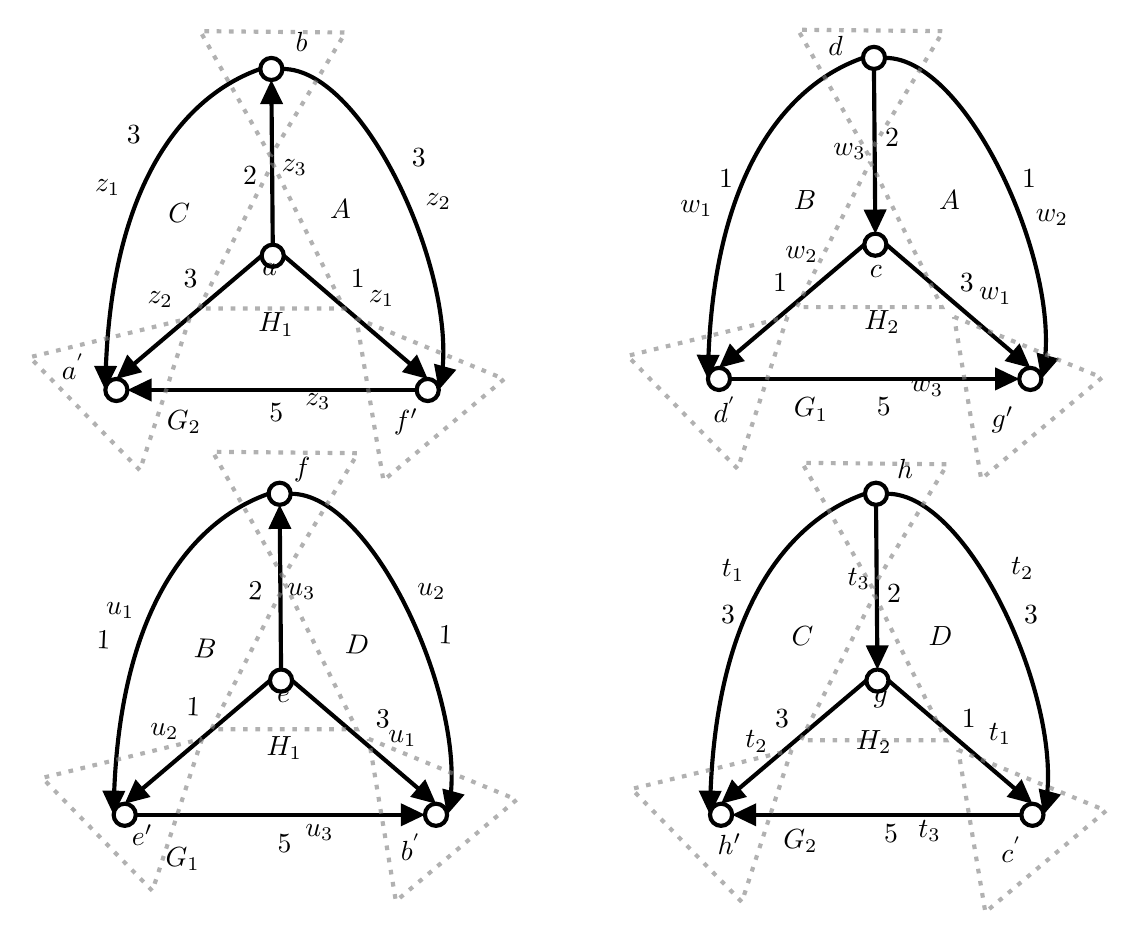
\begin{tikzpicture}[x=0.75pt,y=0.75pt,yscale=-1,xscale=1]
%uncomment if require: \path (0,498); %set diagram left start at 0, and has height of 498

%Shape: Circle [id:dp5729830365949617] 
\draw  [line width=1.5]  (161.81,25.33) .. controls (161.81,22.39) and (164.2,20) .. (167.14,20) .. controls (170.09,20) and (172.47,22.39) .. (172.47,25.33) .. controls (172.47,28.28) and (170.09,30.67) .. (167.14,30.67) .. controls (164.2,30.67) and (161.81,28.28) .. (161.81,25.33) -- cycle ;
%Shape: Circle [id:dp37612834718030397] 
\draw  [line width=1.5]  (162.47,115.33) .. controls (162.47,112.39) and (164.86,110) .. (167.81,110) .. controls (170.75,110) and (173.14,112.39) .. (173.14,115.33) .. controls (173.14,118.28) and (170.75,120.67) .. (167.81,120.67) .. controls (164.86,120.67) and (162.47,118.28) .. (162.47,115.33) -- cycle ;
%Straight Lines [id:da9158510271719965] 
\draw [line width=1.5]    (167.17,34.67) -- (167.81,110) ;
\draw [shift={(167.14,30.67)}, rotate = 89.52] [fill={rgb, 255:red, 0; green, 0; blue, 0 }  ][line width=0.08]  [draw opacity=0] (11.61,-5.58) -- (0,0) -- (11.61,5.58) -- cycle    ;
%Straight Lines [id:da691738049353374] 
\draw [line width=1.5]    (101.81,180) -- (237.14,180) ;
\draw [shift={(97.81,180)}, rotate = 0] [fill={rgb, 255:red, 0; green, 0; blue, 0 }  ][line width=0.08]  [draw opacity=0] (11.61,-5.58) -- (0,0) -- (11.61,5.58) -- cycle    ;
%Straight Lines [id:da21012216073255352] 
\draw [line width=1.5]    (95.53,172.08) -- (162.47,115.33) ;
\draw [shift={(92.47,174.67)}, rotate = 319.71] [fill={rgb, 255:red, 0; green, 0; blue, 0 }  ][line width=0.08]  [draw opacity=0] (11.61,-5.58) -- (0,0) -- (11.61,5.58) -- cycle    ;
%Straight Lines [id:da7410869854550676] 
\draw [line width=1.5]    (173.14,115.33) -- (239.43,172.07) ;
\draw [shift={(242.47,174.67)}, rotate = 220.56] [fill={rgb, 255:red, 0; green, 0; blue, 0 }  ][line width=0.08]  [draw opacity=0] (11.61,-5.58) -- (0,0) -- (11.61,5.58) -- cycle    ;
%Curve Lines [id:da21492669607570647] 
\draw [line width=1.5]    (87.21,175.61) .. controls (89.24,80.37) and (125.36,38.14) .. (161.81,25.33) ;
\draw [shift={(87.14,180)}, rotate = 270.58] [fill={rgb, 255:red, 0; green, 0; blue, 0 }  ][line width=0.08]  [draw opacity=0] (11.61,-5.58) -- (0,0) -- (11.61,5.58) -- cycle    ;
%Curve Lines [id:da9036325885810722] 
\draw [line width=1.5]    (172.47,25.33) .. controls (212.45,25.01) and (258.44,127.03) .. (248.67,176.32) ;
\draw [shift={(247.81,180)}, rotate = 285.26] [fill={rgb, 255:red, 0; green, 0; blue, 0 }  ][line width=0.08]  [draw opacity=0] (11.61,-5.58) -- (0,0) -- (11.61,5.58) -- cycle    ;
%Shape: Circle [id:dp6426609962699884] 
\draw  [line width=1.5]  (87.14,180) .. controls (87.14,177.05) and (89.53,174.67) .. (92.47,174.67) .. controls (95.42,174.67) and (97.81,177.05) .. (97.81,180) .. controls (97.81,182.95) and (95.42,185.33) .. (92.47,185.33) .. controls (89.53,185.33) and (87.14,182.95) .. (87.14,180) -- cycle ;
%Shape: Circle [id:dp45710635129265853] 
\draw  [line width=1.5]  (237.14,180) .. controls (237.14,177.05) and (239.53,174.67) .. (242.47,174.67) .. controls (245.42,174.67) and (247.81,177.05) .. (247.81,180) .. controls (247.81,182.95) and (245.42,185.33) .. (242.47,185.33) .. controls (239.53,185.33) and (237.14,182.95) .. (237.14,180) -- cycle ;
%Shape: Circle [id:dp9010615426685297] 
\draw  [line width=1.5]  (165.81,230) .. controls (165.81,227.05) and (168.2,224.67) .. (171.14,224.67) .. controls (174.09,224.67) and (176.47,227.05) .. (176.47,230) .. controls (176.47,232.95) and (174.09,235.33) .. (171.14,235.33) .. controls (168.2,235.33) and (165.81,232.95) .. (165.81,230) -- cycle ;
%Shape: Circle [id:dp8341928324956512] 
\draw  [line width=1.5]  (166.47,320) .. controls (166.47,317.05) and (168.86,314.67) .. (171.81,314.67) .. controls (174.75,314.67) and (177.14,317.05) .. (177.14,320) .. controls (177.14,322.95) and (174.75,325.33) .. (171.81,325.33) .. controls (168.86,325.33) and (166.47,322.95) .. (166.47,320) -- cycle ;
%Shape: Circle [id:dp7263331520607497] 
\draw  [line width=1.5]  (241.14,384.67) .. controls (241.14,381.72) and (243.53,379.33) .. (246.47,379.33) .. controls (249.42,379.33) and (251.81,381.72) .. (251.81,384.67) .. controls (251.81,387.61) and (249.42,390) .. (246.47,390) .. controls (243.53,390) and (241.14,387.61) .. (241.14,384.67) -- cycle ;
%Straight Lines [id:da9896464315387669] 
\draw [line width=1.5]    (171.17,239.33) -- (171.81,314.67) ;
\draw [shift={(171.14,235.33)}, rotate = 89.52] [fill={rgb, 255:red, 0; green, 0; blue, 0 }  ][line width=0.08]  [draw opacity=0] (11.61,-5.58) -- (0,0) -- (11.61,5.58) -- cycle    ;
%Straight Lines [id:da3068077560217968] 
\draw [line width=1.5]    (101.81,384.67) -- (237.14,384.67) ;
\draw [shift={(241.14,384.67)}, rotate = 180] [fill={rgb, 255:red, 0; green, 0; blue, 0 }  ][line width=0.08]  [draw opacity=0] (11.61,-5.58) -- (0,0) -- (11.61,5.58) -- cycle    ;
%Straight Lines [id:da1192544795528433] 
\draw [line width=1.5]    (99.53,376.75) -- (166.47,320) ;
\draw [shift={(96.47,379.33)}, rotate = 319.71] [fill={rgb, 255:red, 0; green, 0; blue, 0 }  ][line width=0.08]  [draw opacity=0] (11.61,-5.58) -- (0,0) -- (11.61,5.58) -- cycle    ;
%Straight Lines [id:da5014217572994905] 
\draw [line width=1.5]    (177.14,320) -- (243.43,376.73) ;
\draw [shift={(246.47,379.33)}, rotate = 220.56] [fill={rgb, 255:red, 0; green, 0; blue, 0 }  ][line width=0.08]  [draw opacity=0] (11.61,-5.58) -- (0,0) -- (11.61,5.58) -- cycle    ;
%Curve Lines [id:da14877238718382224] 
\draw [line width=1.5]    (91.21,380.28) .. controls (93.24,285.04) and (129.36,242.81) .. (165.81,230) ;
\draw [shift={(91.14,384.67)}, rotate = 270.58] [fill={rgb, 255:red, 0; green, 0; blue, 0 }  ][line width=0.08]  [draw opacity=0] (11.61,-5.58) -- (0,0) -- (11.61,5.58) -- cycle    ;
%Curve Lines [id:da6788551769771028] 
\draw [line width=1.5]    (176.47,230) .. controls (216.45,229.68) and (262.44,331.7) .. (252.67,380.98) ;
\draw [shift={(251.81,384.67)}, rotate = 285.26] [fill={rgb, 255:red, 0; green, 0; blue, 0 }  ][line width=0.08]  [draw opacity=0] (11.61,-5.58) -- (0,0) -- (11.61,5.58) -- cycle    ;
%Shape: Circle [id:dp8968629678267172] 
\draw  [line width=1.5]  (91.14,384.67) .. controls (91.14,381.72) and (93.53,379.33) .. (96.47,379.33) .. controls (99.42,379.33) and (101.81,381.72) .. (101.81,384.67) .. controls (101.81,387.61) and (99.42,390) .. (96.47,390) .. controls (93.53,390) and (91.14,387.61) .. (91.14,384.67) -- cycle ;
%Shape: Circle [id:dp7197685772792822] 
\draw  [line width=1.5]  (452.14,20) .. controls (452.14,17.05) and (454.53,14.67) .. (457.47,14.67) .. controls (460.42,14.67) and (462.81,17.05) .. (462.81,20) .. controls (462.81,22.95) and (460.42,25.33) .. (457.47,25.33) .. controls (454.53,25.33) and (452.14,22.95) .. (452.14,20) -- cycle ;
%Shape: Circle [id:dp49004728051988067] 
\draw  [line width=1.5]  (452.81,110) .. controls (452.81,107.05) and (455.2,104.67) .. (458.14,104.67) .. controls (461.09,104.67) and (463.47,107.05) .. (463.47,110) .. controls (463.47,112.95) and (461.09,115.33) .. (458.14,115.33) .. controls (455.2,115.33) and (452.81,112.95) .. (452.81,110) -- cycle ;
%Shape: Circle [id:dp9996086110664077] 
\draw  [line width=1.5]  (527.47,174.67) .. controls (527.47,171.72) and (529.86,169.33) .. (532.81,169.33) .. controls (535.75,169.33) and (538.14,171.72) .. (538.14,174.67) .. controls (538.14,177.61) and (535.75,180) .. (532.81,180) .. controls (529.86,180) and (527.47,177.61) .. (527.47,174.67) -- cycle ;
%Straight Lines [id:da5916120908249641] 
\draw [line width=1.5]    (457.47,25.33) -- (458.11,100.67) ;
\draw [shift={(458.14,104.67)}, rotate = 269.52] [fill={rgb, 255:red, 0; green, 0; blue, 0 }  ][line width=0.08]  [draw opacity=0] (11.61,-5.58) -- (0,0) -- (11.61,5.58) -- cycle    ;
%Straight Lines [id:da2675543814820319] 
\draw [line width=1.5]    (388.14,174.67) -- (523.47,174.67) ;
\draw [shift={(527.47,174.67)}, rotate = 180] [fill={rgb, 255:red, 0; green, 0; blue, 0 }  ][line width=0.08]  [draw opacity=0] (11.61,-5.58) -- (0,0) -- (11.61,5.58) -- cycle    ;
%Straight Lines [id:da8619340282694029] 
\draw [line width=1.5]    (385.86,166.75) -- (452.81,110) ;
\draw [shift={(382.81,169.33)}, rotate = 319.71] [fill={rgb, 255:red, 0; green, 0; blue, 0 }  ][line width=0.08]  [draw opacity=0] (11.61,-5.58) -- (0,0) -- (11.61,5.58) -- cycle    ;
%Straight Lines [id:da3311013263120153] 
\draw [line width=1.5]    (463.47,110) -- (529.77,166.73) ;
\draw [shift={(532.81,169.33)}, rotate = 220.56] [fill={rgb, 255:red, 0; green, 0; blue, 0 }  ][line width=0.08]  [draw opacity=0] (11.61,-5.58) -- (0,0) -- (11.61,5.58) -- cycle    ;
%Curve Lines [id:da6945139417973814] 
\draw [line width=1.5]    (377.54,170.28) .. controls (379.57,75.04) and (415.7,32.8) .. (452.14,20) ;
\draw [shift={(377.47,174.67)}, rotate = 270.58] [fill={rgb, 255:red, 0; green, 0; blue, 0 }  ][line width=0.08]  [draw opacity=0] (11.61,-5.58) -- (0,0) -- (11.61,5.58) -- cycle    ;
%Curve Lines [id:da7822794249467356] 
\draw [line width=1.5]    (462.81,20) .. controls (502.78,19.67) and (548.78,121.7) .. (539,170.98) ;
\draw [shift={(538.14,174.67)}, rotate = 285.26] [fill={rgb, 255:red, 0; green, 0; blue, 0 }  ][line width=0.08]  [draw opacity=0] (11.61,-5.58) -- (0,0) -- (11.61,5.58) -- cycle    ;
%Shape: Circle [id:dp6495661214839258] 
\draw  [line width=1.5]  (377.47,174.67) .. controls (377.47,171.72) and (379.86,169.33) .. (382.81,169.33) .. controls (385.75,169.33) and (388.14,171.72) .. (388.14,174.67) .. controls (388.14,177.61) and (385.75,180) .. (382.81,180) .. controls (379.86,180) and (377.47,177.61) .. (377.47,174.67) -- cycle ;
%Shape: Circle [id:dp10015321763196539] 
\draw  [line width=1.5]  (453.14,230) .. controls (453.14,227.05) and (455.53,224.67) .. (458.47,224.67) .. controls (461.42,224.67) and (463.81,227.05) .. (463.81,230) .. controls (463.81,232.95) and (461.42,235.33) .. (458.47,235.33) .. controls (455.53,235.33) and (453.14,232.95) .. (453.14,230) -- cycle ;
%Shape: Circle [id:dp03418543258112594] 
\draw  [line width=1.5]  (453.81,320) .. controls (453.81,317.05) and (456.2,314.67) .. (459.14,314.67) .. controls (462.09,314.67) and (464.47,317.05) .. (464.47,320) .. controls (464.47,322.95) and (462.09,325.33) .. (459.14,325.33) .. controls (456.2,325.33) and (453.81,322.95) .. (453.81,320) -- cycle ;
%Shape: Circle [id:dp7359218836228637] 
\draw  [line width=1.5]  (528.47,384.67) .. controls (528.47,381.72) and (530.86,379.33) .. (533.81,379.33) .. controls (536.75,379.33) and (539.14,381.72) .. (539.14,384.67) .. controls (539.14,387.61) and (536.75,390) .. (533.81,390) .. controls (530.86,390) and (528.47,387.61) .. (528.47,384.67) -- cycle ;
%Straight Lines [id:da3785724466533624] 
\draw [line width=1.5]    (458.47,235.33) -- (459.11,310.67) ;
\draw [shift={(459.14,314.67)}, rotate = 269.52] [fill={rgb, 255:red, 0; green, 0; blue, 0 }  ][line width=0.08]  [draw opacity=0] (11.61,-5.58) -- (0,0) -- (11.61,5.58) -- cycle    ;
%Straight Lines [id:da2697861935808339] 
\draw [line width=1.5]    (393.14,384.67) -- (528.47,384.67) ;
\draw [shift={(389.14,384.67)}, rotate = 0] [fill={rgb, 255:red, 0; green, 0; blue, 0 }  ][line width=0.08]  [draw opacity=0] (11.61,-5.58) -- (0,0) -- (11.61,5.58) -- cycle    ;
%Straight Lines [id:da17453965147392314] 
\draw [line width=1.5]    (386.86,376.75) -- (453.81,320) ;
\draw [shift={(383.81,379.33)}, rotate = 319.71] [fill={rgb, 255:red, 0; green, 0; blue, 0 }  ][line width=0.08]  [draw opacity=0] (11.61,-5.58) -- (0,0) -- (11.61,5.58) -- cycle    ;
%Straight Lines [id:da07864825916900786] 
\draw [line width=1.5]    (464.47,320) -- (530.77,376.73) ;
\draw [shift={(533.81,379.33)}, rotate = 220.56] [fill={rgb, 255:red, 0; green, 0; blue, 0 }  ][line width=0.08]  [draw opacity=0] (11.61,-5.58) -- (0,0) -- (11.61,5.58) -- cycle    ;
%Curve Lines [id:da9315806742362415] 
\draw [line width=1.5]    (378.54,380.28) .. controls (380.57,285.04) and (416.7,242.81) .. (453.14,230) ;
\draw [shift={(378.47,384.67)}, rotate = 270.58] [fill={rgb, 255:red, 0; green, 0; blue, 0 }  ][line width=0.08]  [draw opacity=0] (11.61,-5.58) -- (0,0) -- (11.61,5.58) -- cycle    ;
%Curve Lines [id:da17189628696395065] 
\draw [line width=1.5]    (463.81,230) .. controls (503.78,229.68) and (549.78,331.7) .. (540,380.98) ;
\draw [shift={(539.14,384.67)}, rotate = 285.26] [fill={rgb, 255:red, 0; green, 0; blue, 0 }  ][line width=0.08]  [draw opacity=0] (11.61,-5.58) -- (0,0) -- (11.61,5.58) -- cycle    ;
%Shape: Circle [id:dp47115208809575815] 
\draw  [line width=1.5]  (378.47,384.67) .. controls (378.47,381.72) and (380.86,379.33) .. (383.81,379.33) .. controls (386.75,379.33) and (389.14,381.72) .. (389.14,384.67) .. controls (389.14,387.61) and (386.75,390) .. (383.81,390) .. controls (380.86,390) and (378.47,387.61) .. (378.47,384.67) -- cycle ;
%Shape: Triangle [id:dp6389874267176925] 
\draw  [color={rgb, 255:red, 128; green, 128; blue, 128 }  ,draw opacity=0.61 ][dash pattern={on 1.69pt off 2.76pt}][line width=1.5]  (166.76,67.43) -- (132.85,7.11) -- (202.84,7.79) -- cycle ;
%Shape: Triangle [id:dp36108366327372987] 
\draw  [color={rgb, 255:red, 128; green, 128; blue, 128 }  ,draw opacity=0.61 ][dash pattern={on 1.69pt off 2.76pt}][line width=1.5]  (167.74,70.77) -- (202.24,140.77) -- (132.24,140.77) -- cycle ;
%Shape: Triangle [id:dp7364938247780082] 
\draw  [color={rgb, 255:red, 128; green, 128; blue, 128 }  ,draw opacity=0.61 ][dash pattern={on 1.69pt off 2.76pt}][line width=1.5]  (127.74,145.44) -- (103.8,218.67) -- (50.73,164.22) -- cycle ;
%Shape: Triangle [id:dp8688796137791671] 
\draw  [color={rgb, 255:red, 128; green, 128; blue, 128 }  ,draw opacity=0.61 ][dash pattern={on 1.69pt off 2.76pt}][line width=1.5]  (208.07,145.44) -- (279.33,174.73) -- (221.12,223.63) -- cycle ;
%Shape: Triangle [id:dp5510471902819721] 
\draw  [color={rgb, 255:red, 128; green, 128; blue, 128 }  ,draw opacity=0.61 ][dash pattern={on 1.69pt off 2.76pt}][line width=1.5]  (172.76,270.1) -- (138.85,209.77) -- (208.84,210.46) -- cycle ;
%Shape: Triangle [id:dp5832218749091068] 
\draw  [color={rgb, 255:red, 128; green, 128; blue, 128 }  ,draw opacity=0.61 ][dash pattern={on 1.69pt off 2.76pt}][line width=1.5]  (173.74,273.44) -- (208.24,343.44) -- (138.24,343.44) -- cycle ;
%Shape: Triangle [id:dp17185534363242116] 
\draw  [color={rgb, 255:red, 128; green, 128; blue, 128 }  ,draw opacity=0.61 ][dash pattern={on 1.69pt off 2.76pt}][line width=1.5]  (133.74,348.1) -- (109.8,421.33) -- (56.73,366.89) -- cycle ;
%Shape: Triangle [id:dp5927451881338996] 
\draw  [color={rgb, 255:red, 128; green, 128; blue, 128 }  ,draw opacity=0.61 ][dash pattern={on 1.69pt off 2.76pt}][line width=1.5]  (214.07,348.1) -- (285.33,377.39) -- (227.12,426.29) -- cycle ;
%Shape: Triangle [id:dp22961376462006855] 
\draw  [color={rgb, 255:red, 128; green, 128; blue, 128 }  ,draw opacity=0.61 ][dash pattern={on 1.69pt off 2.76pt}][line width=1.5]  (456.76,275.43) -- (422.85,215.11) -- (492.84,215.79) -- cycle ;
%Shape: Triangle [id:dp7412114645452874] 
\draw  [color={rgb, 255:red, 128; green, 128; blue, 128 }  ,draw opacity=0.61 ][dash pattern={on 1.69pt off 2.76pt}][line width=1.5]  (457.74,278.77) -- (492.24,348.77) -- (422.24,348.77) -- cycle ;
%Shape: Triangle [id:dp5335245159862751] 
\draw  [color={rgb, 255:red, 128; green, 128; blue, 128 }  ,draw opacity=0.61 ][dash pattern={on 1.69pt off 2.76pt}][line width=1.5]  (417.74,353.44) -- (393.8,426.67) -- (340.73,372.22) -- cycle ;
%Shape: Triangle [id:dp6675828844645042] 
\draw  [color={rgb, 255:red, 128; green, 128; blue, 128 }  ,draw opacity=0.61 ][dash pattern={on 1.69pt off 2.76pt}][line width=1.5]  (498.07,353.44) -- (569.33,382.73) -- (511.12,431.63) -- cycle ;
%Shape: Triangle [id:dp7953792568010355] 
\draw  [color={rgb, 255:red, 128; green, 128; blue, 128 }  ,draw opacity=0.61 ][dash pattern={on 1.69pt off 2.76pt}][line width=1.5]  (454.76,66.76) -- (420.85,6.44) -- (490.84,7.13) -- cycle ;
%Shape: Triangle [id:dp43961271511290967] 
\draw  [color={rgb, 255:red, 128; green, 128; blue, 128 }  ,draw opacity=0.61 ][dash pattern={on 1.69pt off 2.76pt}][line width=1.5]  (455.74,70.1) -- (490.24,140.1) -- (420.24,140.1) -- cycle ;
%Shape: Triangle [id:dp24827760567983648] 
\draw  [color={rgb, 255:red, 128; green, 128; blue, 128 }  ,draw opacity=0.61 ][dash pattern={on 1.69pt off 2.76pt}][line width=1.5]  (415.74,144.77) -- (391.8,218) -- (338.73,163.56) -- cycle ;
%Shape: Triangle [id:dp7191718328020039] 
\draw  [color={rgb, 255:red, 128; green, 128; blue, 128 }  ,draw opacity=0.61 ][dash pattern={on 1.69pt off 2.76pt}][line width=1.5]  (496.07,144.77) -- (567.33,174.06) -- (509.12,222.96) -- cycle ;

% Text Node
\draw (159.33,141.4) node [anchor=north west][inner sep=0.75pt]    {$H_{1}$};
% Text Node
\draw (194,86.73) node [anchor=north west][inner sep=0.75pt]    {$A$};
% Text Node
\draw (116,88.73) node [anchor=north west][inner sep=0.75pt]    {$C$};
% Text Node
\draw (115.33,188.4) node [anchor=north west][inner sep=0.75pt]    {$G_{2}$};
% Text Node
\draw (204,120.4) node [anchor=north west][inner sep=0.75pt]    {$1$};
% Text Node
\draw (123.33,120.4) node [anchor=north west][inner sep=0.75pt]    {$3$};
% Text Node
\draw (233.33,62.4) node [anchor=north west][inner sep=0.75pt]    {$3$};
% Text Node
\draw (96,51.07) node [anchor=north west][inner sep=0.75pt]    {$3$};
% Text Node
\draw (152,71.07) node [anchor=north west][inner sep=0.75pt]    {$2$};
% Text Node
\draw (164.67,185.07) node [anchor=north west][inner sep=0.75pt]    {$5$};
% Text Node
\draw (154.9,270.75) node [anchor=north west][inner sep=0.75pt]  [rotate=-2.55]  {$2$};
% Text Node
\draw (201.5,296.09) node [anchor=north west][inner sep=0.75pt]  [rotate=-2.55]  {$D$};
% Text Node
\draw (128.62,298.44) node [anchor=north west][inner sep=0.75pt]  [rotate=-2.55]  {$B$};
% Text Node
\draw (81.84,294.23) node [anchor=north west][inner sep=0.75pt]  [rotate=-2.55]  {$1$};
% Text Node
\draw (246.5,292.23) node [anchor=north west][inner sep=0.75pt]  [rotate=-2.55]  {$1$};
% Text Node
\draw (216.36,332.26) node [anchor=north west][inner sep=0.75pt]  [rotate=-2.55]  {$3$};
% Text Node
\draw (125.05,326.62) node [anchor=north west][inner sep=0.75pt]  [rotate=-2.55]  {$1$};
% Text Node
\draw (163.33,345.4) node [anchor=north west][inner sep=0.75pt]    {$H_{1}$};
% Text Node
\draw (168.67,392.73) node [anchor=north west][inner sep=0.75pt]    {$5$};
% Text Node
\draw (114.67,399.07) node [anchor=north west][inner sep=0.75pt]    {$G_{1}$};
% Text Node
\draw (417.33,82.4) node [anchor=north west][inner sep=0.75pt]    {$B$};
% Text Node
\draw (487.33,82.4) node [anchor=north west][inner sep=0.75pt]    {$A$};
% Text Node
\draw (451.33,140.4) node [anchor=north west][inner sep=0.75pt]    {$H_{2}$};
% Text Node
\draw (417.33,182.4) node [anchor=north west][inner sep=0.75pt]    {$G_{1}$};
% Text Node
\draw (381.33,72.4) node [anchor=north west][inner sep=0.75pt]    {$1$};
% Text Node
\draw (527.33,72.4) node [anchor=north west][inner sep=0.75pt]    {$1$};
% Text Node
\draw (407.33,122.4) node [anchor=north west][inner sep=0.75pt]    {$1$};
% Text Node
\draw (461.33,52.4) node [anchor=north west][inner sep=0.75pt]    {$2$};
% Text Node
\draw (497.33,122.4) node [anchor=north west][inner sep=0.75pt]    {$3$};
% Text Node
\draw (457.33,182.4) node [anchor=north west][inner sep=0.75pt]    {$5$};
% Text Node
\draw (416.33,292.4) node [anchor=north west][inner sep=0.75pt]    {$C$};
% Text Node
\draw (482.33,292.4) node [anchor=north west][inner sep=0.75pt]    {$D$};
% Text Node
\draw (447.33,342.4) node [anchor=north west][inner sep=0.75pt]    {$H_{2}$};
% Text Node
\draw (412.33,390.4) node [anchor=north west][inner sep=0.75pt]    {$G_{2}$};
% Text Node
\draw (382.33,282.4) node [anchor=north west][inner sep=0.75pt]    {$3$};
% Text Node
\draw (528.33,282.4) node [anchor=north west][inner sep=0.75pt]    {$3$};
% Text Node
\draw (408.33,332.4) node [anchor=north west][inner sep=0.75pt]    {$3$};
% Text Node
\draw (460.81,388.07) node [anchor=north west][inner sep=0.75pt]    {$5$};
% Text Node
\draw (462.33,272.4) node [anchor=north west][inner sep=0.75pt]    {$2$};
% Text Node
\draw (498.33,332.4) node [anchor=north west][inner sep=0.75pt]    {$1$};
% Text Node
\draw (212.67,130.4) node [anchor=north west][inner sep=0.75pt]    {$z_{1}$};
% Text Node
\draw (80.67,77.07) node [anchor=north west][inner sep=0.75pt]    {$z_{1}$};
% Text Node
\draw (106,131.07) node [anchor=north west][inner sep=0.75pt]    {$z_{2}$};
% Text Node
\draw (240,83.73) node [anchor=north west][inner sep=0.75pt]    {$z_{2}$};
% Text Node
\draw (170.67,67.4) node [anchor=north west][inner sep=0.75pt]    {$z_{3}$};
% Text Node
\draw (182,180.07) node [anchor=north west][inner sep=0.75pt]    {$z_{3}$};
% Text Node
\draw (506.67,129.4) node [anchor=north west][inner sep=0.75pt]    {$w_{1}$};
% Text Node
\draw (362.67,87.4) node [anchor=north west][inner sep=0.75pt]    {$w_{1}$};
% Text Node
\draw (413.33,109.4) node [anchor=north west][inner sep=0.75pt]    {$w_{2}$};
% Text Node
\draw (534,91.4) node [anchor=north west][inner sep=0.75pt]    {$w_{2}$};
% Text Node
\draw (436.47,59.73) node [anchor=north west][inner sep=0.75pt]    {$w_{3}$};
% Text Node
\draw (473.81,173.73) node [anchor=north west][inner sep=0.75pt]    {$w_{3}$};
% Text Node
\draw (222,342.4) node [anchor=north west][inner sep=0.75pt]    {$u_{1}$};
% Text Node
\draw (86,281.07) node [anchor=north west][inner sep=0.75pt]    {$u_{1}$};
% Text Node
\draw (107.33,339.07) node [anchor=north west][inner sep=0.75pt]    {$u_{2}$};
% Text Node
\draw (236,271.73) node [anchor=north west][inner sep=0.75pt]    {$u_{2}$};
% Text Node
\draw (173.33,271.73) node [anchor=north west][inner sep=0.75pt]    {$u_{3}$};
% Text Node
\draw (182,387.73) node [anchor=north west][inner sep=0.75pt]    {$u_{3}$};
% Text Node
\draw (511.33,339.07) node [anchor=north west][inner sep=0.75pt]    {$t_{1}$};
% Text Node
\draw (382.67,260.4) node [anchor=north west][inner sep=0.75pt]    {$t_{1}$};
% Text Node
\draw (394,342.73) node [anchor=north west][inner sep=0.75pt]    {$t_{2}$};
% Text Node
\draw (522,259.4) node [anchor=north west][inner sep=0.75pt]    {$t_{2}$};
% Text Node
\draw (443.33,264.4) node [anchor=north west][inner sep=0.75pt]    {$t_{3}$};
% Text Node
\draw (477.33,385.73) node [anchor=north west][inner sep=0.75pt]    {$t_{3}$};
% Text Node
\draw (161.33,117.4) node [anchor=north west][inner sep=0.75pt]    {$a$};
% Text Node
\draw (177.33,6.07) node [anchor=north west][inner sep=0.75pt]    {$b$};
% Text Node
\draw (454,118.73) node [anchor=north west][inner sep=0.75pt]    {$c$};
% Text Node
\draw (434,8.07) node [anchor=north west][inner sep=0.75pt]    {$d$};
% Text Node
\draw (176.47,210.73) node [anchor=north west][inner sep=0.75pt]    {$f$};
% Text Node
\draw (455.81,323.4) node [anchor=north west][inner sep=0.75pt]    {$g$};
% Text Node
\draw (467.14,212.07) node [anchor=north west][inner sep=0.75pt]    {$h$};
% Text Node
\draw (168.47,323.4) node [anchor=north west][inner sep=0.75pt]    {$e$};
% Text Node
\draw (64.67,161.07) node [anchor=north west][inner sep=0.75pt]    {$a^{'}$};
% Text Node
\draw (228,392.4) node [anchor=north west][inner sep=0.75pt]    {$b^{'}$};
% Text Node
\draw (517.33,393.73) node [anchor=north west][inner sep=0.75pt]    {$c^{'}$};
% Text Node
\draw (378.67,181.73) node [anchor=north west][inner sep=0.75pt]    {$d^{'}$};
% Text Node
\draw (98.47,388.07) node [anchor=north west][inner sep=0.75pt]    {$e'$};
% Text Node
\draw (224.67,187.73) node [anchor=north west][inner sep=0.75pt]    {$f'$};
% Text Node
\draw (512.67,186.73) node [anchor=north west][inner sep=0.75pt]    {$g'$};
% Text Node
\draw (380.67,392.4) node [anchor=north west][inner sep=0.75pt]    {$h'$};


\end{tikzpicture}
    \caption{Triangulos en los tetraedros truncados que representan las cuspides}
\end{figure}
Pegando de manera adecuada obtenemos dos paralelogramos que nos representan cada frontera de cúspide como se muestra a continuación
\begin{figure}[H]
\centering
%!TEX root = ./main.tex



\tikzset{every picture/.style={line width=0.75pt}} %set default line width to 0.75pt        

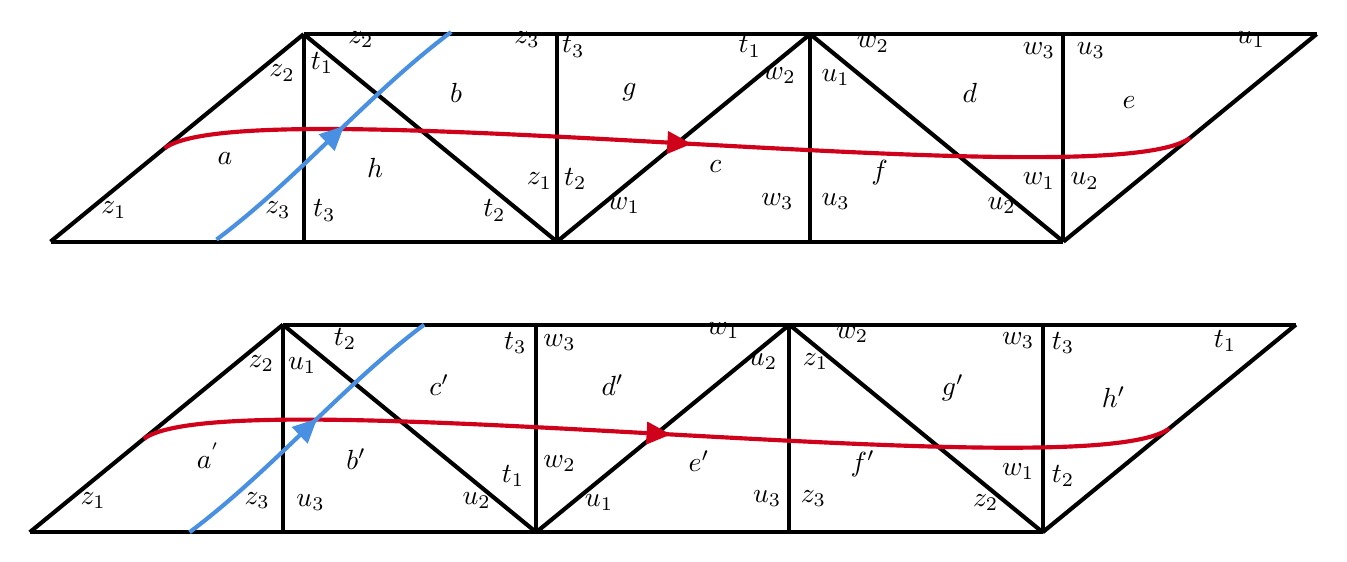
\begin{tikzpicture}[x=0.75pt,y=0.75pt,yscale=-1,xscale=1]
%uncomment if require: \path (0,542); %set diagram left start at 0, and has height of 542

%Straight Lines [id:da13006069871416692] 
\draw [line width=1.5]    (142,195) -- (630,195) ;
%Straight Lines [id:da13561558542782937] 
\draw [line width=1.5]    (142,195) -- (20,295) ;
%Straight Lines [id:da6048067045021074] 
\draw [line width=1.5]    (630,195) -- (508,295) ;
%Straight Lines [id:da7479845165592521] 
\draw [line width=1.5]    (20,295) -- (508,295) ;
%Straight Lines [id:da5146924711453463] 
\draw [line width=1.5]    (142,195) -- (142,295) ;
%Straight Lines [id:da7683491262763936] 
\draw [line width=1.5]    (264,195) -- (264,295) ;
%Straight Lines [id:da15527473375540246] 
\draw [line width=1.5]    (386,195) -- (386,295) ;
%Straight Lines [id:da45625934758008424] 
\draw [line width=1.5]    (508,195) -- (508,295) ;
%Straight Lines [id:da3616387902013627] 
\draw [line width=1.5]    (386,195) -- (264,295) ;
%Straight Lines [id:da044739648304707336] 
\draw [line width=1.5]    (264,295) -- (142,195) ;
%Straight Lines [id:da2836418136045904] 
\draw [line width=1.5]    (508,295) -- (386,195) ;
%Straight Lines [id:da867664282695949] 
\draw [line width=1.5]    (152,55) -- (640,55) ;
%Straight Lines [id:da9918221704170823] 
\draw [line width=1.5]    (152,55) -- (30,155) ;
%Straight Lines [id:da5944725906481361] 
\draw [line width=1.5]    (640,55) -- (518,155) ;
%Straight Lines [id:da8733020176164918] 
\draw [line width=1.5]    (30,155) -- (518,155) ;
%Straight Lines [id:da8720752195824351] 
\draw [line width=1.5]    (152,55) -- (152,155) ;
%Straight Lines [id:da9117542313308579] 
\draw [line width=1.5]    (274,55) -- (274,155) ;
%Straight Lines [id:da28083917441028194] 
\draw [line width=1.5]    (396,55) -- (396,155) ;
%Straight Lines [id:da06592295243917656] 
\draw [line width=1.5]    (518,55) -- (518,155) ;
%Straight Lines [id:da9134925142291349] 
\draw [line width=1.5]    (396,55) -- (274,155) ;
%Straight Lines [id:da022240721894983384] 
\draw [line width=1.5]    (274,155) -- (152,55) ;
%Straight Lines [id:da6293934000840508] 
\draw [line width=1.5]    (518,155) -- (396,55) ;
%Curve Lines [id:da5316729016494588] 
\draw [color={rgb, 255:red, 208; green, 2; blue, 27 }  ,draw opacity=1 ][line width=1.5]    (85,110) .. controls (125,80) and (539,135) .. (579,105) ;
\draw [shift={(338.81,107.87)}, rotate = 183.15] [fill={rgb, 255:red, 208; green, 2; blue, 27 }  ,fill opacity=1 ][line width=0.08]  [draw opacity=0] (11.61,-5.58) -- (0,0) -- (11.61,5.58) -- cycle    ;
%Curve Lines [id:da09367095573809125] 
\draw [color={rgb, 255:red, 208; green, 2; blue, 27 }  ,draw opacity=1 ][line width=1.5]    (75,250) .. controls (115,220) and (529,275) .. (569,245) ;
\draw [shift={(328.81,247.87)}, rotate = 183.15] [fill={rgb, 255:red, 208; green, 2; blue, 27 }  ,fill opacity=1 ][line width=0.08]  [draw opacity=0] (11.61,-5.58) -- (0,0) -- (11.61,5.58) -- cycle    ;
%Curve Lines [id:da08706634222859888] 
\draw [color={rgb, 255:red, 74; green, 144; blue, 226 }  ,draw opacity=1 ][line width=1.5]    (110,154) .. controls (150,124) and (183,84) .. (223,54) ;
\draw [shift={(171.43,99.28)}, rotate = 136.23] [fill={rgb, 255:red, 74; green, 144; blue, 226 }  ,fill opacity=1 ][line width=0.08]  [draw opacity=0] (11.61,-5.58) -- (0,0) -- (11.61,5.58) -- cycle    ;
%Curve Lines [id:da3000463539903655] 
\draw [color={rgb, 255:red, 74; green, 144; blue, 226 }  ,draw opacity=1 ][line width=1.5]    (97,295) .. controls (137,265) and (170,225) .. (210,195) ;
\draw [shift={(158.43,240.28)}, rotate = 136.23] [fill={rgb, 255:red, 74; green, 144; blue, 226 }  ,fill opacity=1 ][line width=0.08]  [draw opacity=0] (11.61,-5.58) -- (0,0) -- (11.61,5.58) -- cycle    ;

% Text Node
\draw (99,250.4) node [anchor=north west][inner sep=0.75pt]    {$a^{'}$};
% Text Node
\draw (122,274.4) node [anchor=north west][inner sep=0.75pt]    {$z_{3}$};
% Text Node
\draw (124,208.4) node [anchor=north west][inner sep=0.75pt]    {$z_{2}$};
% Text Node
\draw (43,274.4) node [anchor=north west][inner sep=0.75pt]    {$z_{1}$};
% Text Node
\draw (171,253.4) node [anchor=north west][inner sep=0.75pt]    {$b'$};
% Text Node
\draw (147,275.4) node [anchor=north west][inner sep=0.75pt]    {$u_{3}$};
% Text Node
\draw (143,209.4) node [anchor=north west][inner sep=0.75pt]    {$u_{1}$};
% Text Node
\draw (227,274.4) node [anchor=north west][inner sep=0.75pt]    {$u_{2}$};
% Text Node
\draw (211,217.4) node [anchor=north west][inner sep=0.75pt]    {$c'$};
% Text Node
\draw (246,261.4) node [anchor=north west][inner sep=0.75pt]    {$t_{1}$};
% Text Node
\draw (247,197.4) node [anchor=north west][inner sep=0.75pt]    {$t_{3}$};
% Text Node
\draw (165,195.4) node [anchor=north west][inner sep=0.75pt]    {$t_{2}$};
% Text Node
\draw (294,217.4) node [anchor=north west][inner sep=0.75pt]    {$d'$};
% Text Node
\draw (266,198.4) node [anchor=north west][inner sep=0.75pt]    {$w_{3}$};
% Text Node
\draw (266,256.4) node [anchor=north west][inner sep=0.75pt]    {$w_{2}$};
% Text Node
\draw (345,192.4) node [anchor=north west][inner sep=0.75pt]    {$w_{1}$};
% Text Node
\draw (336,254.4) node [anchor=north west][inner sep=0.75pt]    {$e'$};
% Text Node
\draw (365,207.4) node [anchor=north west][inner sep=0.75pt]    {$u_{2}$};
% Text Node
\draw (367,273.4) node [anchor=north west][inner sep=0.75pt]    {$u_{3}$};
% Text Node
\draw (286,275.4) node [anchor=north west][inner sep=0.75pt]    {$u_{1}$};
% Text Node
\draw (414,254.4) node [anchor=north west][inner sep=0.75pt]    {$f'$};
% Text Node
\draw (391,207.4) node [anchor=north west][inner sep=0.75pt]    {$z_{1}$};
% Text Node
\draw (390,273.4) node [anchor=north west][inner sep=0.75pt]    {$z_{3}$};
% Text Node
\draw (473,275.4) node [anchor=north west][inner sep=0.75pt]    {$z_{2}$};
% Text Node
\draw (458,217.4) node [anchor=north west][inner sep=0.75pt]    {$g'$};
% Text Node
\draw (487,260.4) node [anchor=north west][inner sep=0.75pt]    {$w_{1}$};
% Text Node
\draw (407,194.4) node [anchor=north west][inner sep=0.75pt]    {$w_{2}$};
% Text Node
\draw (487,197.4) node [anchor=north west][inner sep=0.75pt]    {$w_{3}$};
% Text Node
\draw (535,223.4) node [anchor=north west][inner sep=0.75pt]    {$h'$};
% Text Node
\draw (511,261.4) node [anchor=north west][inner sep=0.75pt]    {$t_{2}$};
% Text Node
\draw (511,197.4) node [anchor=north west][inner sep=0.75pt]    {$t_{3}$};
% Text Node
\draw (589,196.4) node [anchor=north west][inner sep=0.75pt]    {$t_{1}$};
% Text Node
\draw (109,110.4) node [anchor=north west][inner sep=0.75pt]    {$a$};
% Text Node
\draw (132,134.4) node [anchor=north west][inner sep=0.75pt]    {$z_{3}$};
% Text Node
\draw (134,68.4) node [anchor=north west][inner sep=0.75pt]    {$z_{2}$};
% Text Node
\draw (53,134.4) node [anchor=north west][inner sep=0.75pt]    {$z_{1}$};
% Text Node
\draw (181,113.4) node [anchor=north west][inner sep=0.75pt]    {$h$};
% Text Node
\draw (400,130.4) node [anchor=north west][inner sep=0.75pt]    {$u_{3}$};
% Text Node
\draw (400,70.4) node [anchor=north west][inner sep=0.75pt]    {$u_{1}$};
% Text Node
\draw (480,132.4) node [anchor=north west][inner sep=0.75pt]    {$u_{2}$};
% Text Node
\draw (221,77.4) node [anchor=north west][inner sep=0.75pt]    {$b$};
% Text Node
\draw (154,62.4) node [anchor=north west][inner sep=0.75pt]    {$t_{1}$};
% Text Node
\draw (155,133.4) node [anchor=north west][inner sep=0.75pt]    {$t_{3}$};
% Text Node
\draw (237,133.4) node [anchor=north west][inner sep=0.75pt]    {$t_{2}$};
% Text Node
\draw (304,77.4) node [anchor=north west][inner sep=0.75pt]    {$g$};
% Text Node
\draw (371,130.4) node [anchor=north west][inner sep=0.75pt]    {$w_{3}$};
% Text Node
\draw (372,69.4) node [anchor=north west][inner sep=0.75pt]    {$w_{2}$};
% Text Node
\draw (297,132.4) node [anchor=north west][inner sep=0.75pt]    {$w_{1}$};
% Text Node
\draw (346,114.4) node [anchor=north west][inner sep=0.75pt]    {$c$};
% Text Node
\draw (520,120.4) node [anchor=north west][inner sep=0.75pt]    {$u_{2}$};
% Text Node
\draw (523,57.4) node [anchor=north west][inner sep=0.75pt]    {$u_{3}$};
% Text Node
\draw (600,52.4) node [anchor=north west][inner sep=0.75pt]    {$u_{1}$};
% Text Node
\draw (424,114.4) node [anchor=north west][inner sep=0.75pt]    {$f$};
% Text Node
\draw (258,120.4) node [anchor=north west][inner sep=0.75pt]    {$z_{1}$};
% Text Node
\draw (252,52.4) node [anchor=north west][inner sep=0.75pt]    {$z_{3}$};
% Text Node
\draw (172,52.4) node [anchor=north west][inner sep=0.75pt]    {$z_{2}$};
% Text Node
\draw (468,77.4) node [anchor=north west][inner sep=0.75pt]    {$d$};
% Text Node
\draw (497,120.4) node [anchor=north west][inner sep=0.75pt]    {$w_{1}$};
% Text Node
\draw (417,54.4) node [anchor=north west][inner sep=0.75pt]    {$w_{2}$};
% Text Node
\draw (497,57.4) node [anchor=north west][inner sep=0.75pt]    {$w_{3}$};
% Text Node
\draw (545,83.4) node [anchor=north west][inner sep=0.75pt]    {$e$};
% Text Node
\draw (276,118.4) node [anchor=north west][inner sep=0.75pt]    {$t_{2}$};
% Text Node
\draw (275,54.4) node [anchor=north west][inner sep=0.75pt]    {$t_{3}$};
% Text Node
\draw (360,54.4) node [anchor=north west][inner sep=0.75pt]    {$t_{1}$};


\end{tikzpicture}
    \caption{Triangulación de las cúspides y curvas generadoras}
\end{figure}
Observe que de una vez en cada cúspide trazamos las curvas que generan el grupo fundamental, en rojo $\alpha,\alpha^\prime$ y en azul $\beta,\beta^\prime$. Así el numero asociado a cada curva es
\begin{itemize}
    \item $H(\alpha)=z_2t_1z_1^{-1}t_2^{-1}w_2u_1w_1^{-1}u_2^{-1}=\dfrac{z_2t_1w_2u_1}{z_1t_2w_1u_2}.$
    \item $H(\beta)=z_3^{-1}z_2t_1=\dfrac{z_2t_1}{z_3}.$
    \item $H(\alpha^\prime)=z_2u_1t_1^{-1}w_2^{-1}u_2z_1w_1^{-1}t_2^{-1}=\dfrac{z_2u_1u_2z_1}{t_1w_2w_1t_2}.$
    \item $H(\beta^\prime)=z_3^{-1}u_1t_2=\dfrac{u_1t_2}{z_3}$
\end{itemize}
Usando las relaciones de de invariantes de aristas obtenemos las ecuaciones de completez que complementan a las de pegado halladas antes
$$\begin{cases}
    \dfrac{ut(1-u)(1-t)}{zw(1-z)(1-w)}=1\\
    \\
    -\dfrac{zt}{(z-1)^2}=1\\
    \\
    \dfrac{uz(1-w)(1-t)}{tw(1-z)(1-u)}=1\\
    \\
    \dfrac{uz}{(z-1)(1-t)}=1
\end{cases}$$
Nuevamente hallar soluciones a mano seria excesivamente engorroso y para esto es mejor usar herramientas computacionales, pero note que esto nos describe en su totalidad los valores que puede tomar cada invariante de arista, por lo que si uno quisiera unos números en particular basta con remplazar y verificar que todo se cumple.